% !TEX TS-program = xelatex
\RequirePackage[l2tabu,orthodox]{nag} % Раскомментировав, можно в логе получать рекомендации относительно правильного использования пакетов и предупреждения об устаревших и нерекомендуемых пакетах

% Откомментируйте, чтобы отключить генерацию закладок в pdf
% \PassOptionsToPackage{bookmarks=false}{hyperref}
%\documentclass[a5paper,10pt,twoside,openany,article]{memoir}
\documentclass[a4paper,14pt,oneside,openany]{memoir}
% не нужно делать зеркальные страницы, обычный А4 формат, там шрифт 14 т.к., при отправке на печать типография сама уменьшает масштаб


%%% Вывод типов ссылок в библиографии %%%
\makeatletter
\@ifundefined{c@mediadisplay}{
	\newcounter{mediadisplay}
	\setcounter{mediadisplay}{0}
	% 0 --- не делать ничего; надписи [Текст] и [Эл. ресурс] будут выводиться только в ссылках с заполненным полем `media`;
	% 1 --- автоматически добавлять надпись [Текст] к ссылкам с незаполненным полем `media`; таким образом, у всех источников будет указан тип, что соответствует требованиям ГОСТ
	% 2 --- автоматически удалять надписи [Текст], [Эл. Ресурс] и др.; не соответствует ГОСТ
	% 3 --- автоматически удалять надпись [Текст]; не соответствует ГОСТ
	% 4 --- автоматически удалять надпись [Эл. Ресурс]; не соответствует ГОСТ
}{}
\makeatother


% %%% INSTRUCTIONS %%%
% 1) Ссылки с архива, как и любого другого эл. ресурса, нужно будет определить как @online вместо дефолтного @article из школяра.
% 2) Обязательно нужно добавить два поля: url и urldate, чтобы появились требуемые ГОСТом адрес электронного ресурса и дата последнего посещения. Пример:
%		url={https://arxiv.org/abs/2502.17029},
% 		urldate={2025-09-21},
% 3) Поле типа "journal={arXiv preprint arXiv:1412.6980}" можно удалить, так как эта информация более не нужна. Опционально можно перенести содержимое в поле howpublished, но я так не делал.
% 4) Обязательно нужно было добавлять поле "media={eresource}", чтобы появилась требуемая ГОСТом пометка "[Electronic Resource]", но я добавил ниже код в \DeclareSourcemap{...}, который добавляет это поле в каждый @online автоматически.
          % общие настройки шаблона
\newif\ifsynopsis           % Условие, проверяющее, что документ --- автореферат


%%% Основные пакеты %%%
\usepackage{etoolbox}  % для проверки условий, оставляем для возможного расширения
\usepackage{comment}   % для возможности исключать блоки текста


%%% Поля и разметка страницы %%%
\usepackage{geometry}  % задание полей
\usepackage{pdflscape} % альбомные страницы с корректной ориентацией PDF
% \usepackage{lscape} % простая альбомная ориентация


%%% Математика %%%
\usepackage{amsmath,amssymb,amsfonts,amsthm,amscd}
\usepackage{mathtools}  % multlined и др.
\usepackage{xfrac}      % красивые дроби
\usepackage[
locale = DE,
list-separator       = {;\,},
list-final-separator = {;\,},
list-pair-separator  = {;\,},
list-units           = single,
range-units          = single,
range-phrase={\text{\ensuremath{-}}},
fraction-function    = \sfrac,
separate-uncertainty,
]{siunitx}[=v2]
\sisetup{inter-unit-product = \ensuremath{{}\cdot{}}}


%%%% Установки для размера шрифта 14 pt %%%%
%% Формирование переменных и констант для сравнения (один раз для всех подключаемых файлов)%%
%% должно располагаться до вызова пакета fontspec или polyglossia, потому что они сбивают его работу
\newlength{\curtextsize}
\newlength{\bigtextsize}
\setlength{\bigtextsize}{13.9pt}

\makeatletter
%\show\f@size    % неплохо для отслеживания, но вызывает стопорение процесса,
% если документ компилируется без команды  -interaction=nonstopmode
\setlength{\curtextsize}{\f@size pt}
\makeatother


%%% Кодировки и шрифты %%%
\usepackage{polyglossia}         % поддержка многоязычности
\setmainlanguage{english}        % основной язык
\setotherlanguage{russian}       % если вдруг нужен русский

\PassOptionsToPackage{no-math}{fontspec} % опция для fontspec, если нужны математические шрифты
\usepackage{fontspec} % шрифты для XeLaTeX

% Базовые шрифты (обычно нужно скачивать):
\setmainfont{Times New Roman} % ГОСТовский стандартный шрифт
\setsansfont{Arial}
\setmonofont{Courier New}[Scale=0.87] % подгоняет высоту под основной текст (по версии ChatGPT)
% Обеспечиваем кириллицу для этих семейств
\newfontfamily\cyrillicfont{Times New Roman}
\newfontfamily\cyrillicfontsf{Arial}
\newfontfamily\cyrillicfonttt{Courier New}[Scale=0.87]

% Публично доступные аналоги в Debian/Ubuntu:
%\setmainfont{Liberation Serif} % альтернативный свободный аналог Times
%\setsansfont{Liberation Sans}
%\setmonofont{Liberation Mono}[Scale=0.87]
%% Обеспечиваем кириллицу для этих семейств
%\newfontfamily\cyrillicfont{Liberation Serif}
%\newfontfamily\cyrillicfontsf{Liberation Sans}
%\newfontfamily\cyrillicfonttt{Liberation Mono}[Scale=0.87]


%%% Абзацы %%%
\indentafterchapter  % Красная строка после заголовков типа chapter
\usepackage{indentfirst}  % Отступ в первом абзаце после секций/глав
% TODO: как будто после секций не работает


%%% Цвета (если нужно для таблиц/графиков) %%%
\usepackage[dvipsnames]{xcolor}


%%% Таблицы %%%
\usepackage{longtable,ltcaption} % Длинные таблицы
\usepackage{multirow,makecell}   % Улучшенное форматирование таблиц
\usepackage{tabu, tabulary}      % таблицы с автоматически подбирающейся
% шириной столбцов (tabu обязательно
% до hyperref вызывать)

\makeatletter
%https://github.com/tabu-issues-for-future-maintainer/tabu/issues/26
\@ifpackagelater{longtable}{2020/02/07}{
	\def\tabuendlongtrial{%
		\LT@echunk  \global\setbox\LT@gbox \hbox{\unhbox\LT@gbox}\kern\wd\LT@gbox
		\LT@get@widths
	}%
}{}
\makeatother

\usepackage{threeparttable}      % автоматический подгон ширины подписи таблицы


%%% Общие утилиты %%%
%\usepackage{soulutf8}	% soulutf8.sty: warning: 29: This package is obsolete, use the soul package directly.
\usepackage{soul}		% Поддержка переносоустойчивых подчёркиваний и зачёркиваний
\usepackage{icomma}  	% Запятая в десятичных дробях
\usepackage[hyphenation,lastparline]{impnattypo} % Оптимизация расстановки переносов и длины последней строки абзаца


%%% Гиперссылки %%%
\let\CYRDZE\relax
%\usepackage[draft]{hyperref}
\usepackage{hyperref}
%\usepackage{hyperref}%[2012/11/06]


%%% Изображения %%%
\usepackage{graphicx}%[2014/04/25]  % Подключаем пакет работы с графикой
\usepackage{caption}                % Подписи рисунков и таблиц
\usepackage{subcaption}             % Подписи подрисунков и подтаблиц
\usepackage{pdfpages}               % Добавление внешних pdf файлов
\usepackage[export]{adjustbox}


%%% Счётчики %%%
\usepackage{aliascnt}
\usepackage[figure,table]{totalcount}   % Счётчик рисунков и таблиц
\usepackage{totcount}   % Пакет создания счётчиков на основе последнего номера
% подсчитываемого элемента (может требовать дважды
% компилировать документ)
% \usepackage{totpages}   % Счётчик страниц, совместимый с hyperref (ссылается
% на номер последней страницы). Желательно ставить
% последним пакетом в преамбуле


%%% Продвинутое управление групповыми ссылками (пока только формулами) %%%
\usepackage{cleveref}   % продвинутое управление ссылками
\usepackage{kvsetkeys}  % для корректной обработки пробелов в \label
% Добавление возможности использования пробелов в \labelcref
% https://tex.stackexchange.com/a/340502/104425
\makeatletter
\let\org@@cref\@cref
\renewcommand*{\@cref}[2]{%
	\edef\process@me{%
		\noexpand\org@@cref{#1}{\zap@space#2 \@empty}%
	}\process@me
}
\makeatother

\usepackage{placeins} % для \FloatBarrier


%%% User-specific packages %%%
\usepackage{upgreek} % прямые греческие ради русской традиции
\usepackage{pifont}         % adds nice "v" and "x" symbols
\usepackage{bbm}
%\usepackage[ruled]{algorithm2e}       % Пакеты общие для диссертации и автореферата
%\synopsistrue                 % Этот документ --- автореферат
\synopsisfalse                      		% Этот документ --- не автореферат

%%% Прикладные пакеты %%%
%\usepackage{calc}               % Пакет для расчётов параметров, например длины

%%% Для добавления Стр. над номерами страниц в оглавлении
%%% http://tex.stackexchange.com/a/306950
\usepackage{afterpage}

%%% Списки %%%
\usepackage{enumitem}

%%% Оформление списка обозначений
\usepackage[intoc]{nomencl}
\makenomenclature
\setlength{\nomitemsep}{-.8\parsep}
 		% Пакеты только для диссертации
%%%%%%%%%%%%%%%%%%%%%%%%%%%%%%%%%%%%%%%%%%%%%%%%%%%%%%
%%%% Файл упрощённых настроек шаблона диссертации %%%%
%%%%%%%%%%%%%%%%%%%%%%%%%%%%%%%%%%%%%%%%%%%%%%%%%%%%%%

%%% Инициализирование переменных, не трогать!  %%%
\newcounter{intvl}
\newcounter{otstup}
\newcounter{contnumeq}
\newcounter{contnumfig}
\newcounter{contnumtab}
\newcounter{pgnum}
\newcounter{chapstyle}
\newcounter{headingdelim}
\newcounter{headingalign}
\newcounter{headingsize}
%%%%%%%%%%%%%%%%%%%%%%%%%%%%%%%%%%%%%%%%%%%%%%%%%%%%%%


%%% Область упрощённого управления оформлением %%%

%% Интервал между заголовками и между заголовком и текстом %%
% Заголовки отделяют от текста сверху и снизу
% тремя интервалами (ГОСТ Р 7.0.11-2011, 5.3.5)
\setcounter{intvl}{3}               % Коэффициент кратности к размеру шрифта

%% Отступы у заголовков в тексте %%
\setcounter{otstup}{0}              % 0 --- без отступа; 1 --- абзацный отступ

%% Нумерация формул, таблиц и рисунков %%
% Нумерация формул
\setcounter{contnumeq}{0}   % 0 --- пораздельно (во введении подряд, без номера раздела);
% 1 --- сквозная нумерация по всей диссертации
% Нумерация рисунков
\setcounter{contnumfig}{0}  % 0 --- пораздельно (во введении подряд, без номера раздела);
% 1 --- сквозная нумерация по всей диссертации
% Нумерация таблиц
\setcounter{contnumtab}{0}  % 0 --- пораздельно (во введении подряд, без номера раздела);
% 1 --- сквозная нумерация по всей диссертации

%% Оглавление %%
\setcounter{pgnum}{1}       % 0 --- номера страниц никак не обозначены;
% 1 --- Стр. над номерами страниц (дважды компилировать после изменения настройки)
\settocdepth{subsection}    % до какого уровня подразделов выносить в оглавление
\setsecnumdepth{subsection} % до какого уровня нумеровать подразделы

%% Текст и форматирование заголовков %%
\setcounter{chapstyle}{1}     % 0 --- разделы только под номером;
% 1 --- разделы с названием "Глава" перед номером
\setcounter{headingdelim}{0}  % 0 --- номер отделен пропуском в 1em или \quad; сам ГОСТ написан по этому правилу
% 1 --- номера разделов и приложений отделены точкой с пробелом, подразделы пропуском без точки;
% 2 --- номера разделов, подразделов и приложений отделены точкой с пробелом.

%% Выравнивание заголовков в тексте %%
\setcounter{headingalign}{0}  % 0 --- по центру;
% 1 --- по левому краю

%% Размеры заголовков в тексте %%
\setcounter{headingsize}{0}   % 0 --- по ГОСТ, все всегда 14 пт;
% 1 --- пропорционально изменяющийся размер в зависимости от базового шрифта

%% Подпись таблиц %%
%\newcommand{\tabindent}{0cm} % Смещение строк подписи после первой строки
\newlength{\tabindent}
\setlength{\tabindent}{0cm}   % Более надежное определение длин по версии ChatGPT

% Тип форматирования заголовка таблицы:
\newcommand{\tabformat}{plain} % plain --- название и текст в одной строке
% split --- название и текст в разных строках

%%% Настройки форматирования таблицы `plain`
% Выравнивание по центру подписи, состоящей из одной строки:
\newcommand{\tabsinglecenter}{false} % true  --- выравнивать
% false --- не выравнивать
% Выравнивание подписи таблиц:
\newcommand{\tabjust}{justified} % justified   --- выравнивать как обычный текст («по ширине»)
% centering   --- выравнивать по центру
% centerlast  --- выравнивать по центру только последнюю строку
% centerfirst --- выравнивать по центру только первую строку (не рекомендуется)
% raggedleft  --- выравнивать по правому краю
% raggedright --- выравнивать по левому краю

% Разделитель записи «Таблица #» и названия таблицы
%\newcommand{\tablabelsep}{~\cyrdash\ } % Undefined control sequence in current template
\newcommand{\tablabelsep}{~\textemdash\ } % safer in English

%%% Настройки форматирования таблицы `split`

% Положение названия таблицы:
% \centering   --- выравнивать по центру
% \raggedleft  --- выравнивать по правому краю
% \raggedright --- выравнивать по левому краю
\newcommand{\splitformatlabel}{\raggedleft}

% Положение текста подписи:
% \centering   --- выравнивать по центру
% \raggedleft  --- выравнивать по правому краю
% \raggedright --- выравнивать по левому краю
\newcommand{\splitformattext}{\raggedright}

%% Подпись рисунков %%
%Разделитель записи «Рисунок #» и названия рисунка
%\newcommand{\figlabelsep}{~\cyrdash\ }  % (ГОСТ 2.105, 4.3.1) но Undefined control sequence in current template
\newcommand{\figlabelsep}{~\textemdash\ }


%%% Цвета гиперссылок %%%
% Latex color definitions: http://latexcolor.com/
% \definecolor{linkcolor}{rgb}{0.9,0,0}
% \definecolor{citecolor}{rgb}{0,0.6,0}
% \definecolor{urlcolor}{rgb}{0,0,1}
\definecolor{linkcolor}{rgb}{0,0,0} %black
\definecolor{citecolor}{rgb}{0,0,0} %black
\definecolor{urlcolor}{rgb}{0,0,0} %black
      		% Упрощённые настройки шаблона
%%%% Опционально %%%
% Следующий пакет может быть полезен, если надо ужать текст, чтобы сам текст не править, но чтобы места он занимал поменьше
%\usepackage{savetrees}

%%% Списки %%%
\usepackage{enumitem}

% Этот пакет может быть полезен для печати текста брошюрой
%\usepackage[print]{booklet}
  % Пакеты для автореферата
%%%%%%%%%%%%%%%%%%%%%%%%%%%%%%%%%%%%%%%%%%%%%%%%%%%%%%%
%%%% Файл упрощённых настроек шаблона автореферата %%%%
%%%%%%%%%%%%%%%%%%%%%%%%%%%%%%%%%%%%%%%%%%%%%%%%%%%%%%%

%%% Инициализирование переменных, не трогать!  %%%
\newcounter{showperssign}
\newcounter{showsecrsign}
\newcounter{showopplead}
%%%%%%%%%%%%%%%%%%%%%%%%%%%%%%%%%%%%%%%%%%%%%%%%%%%%%%%

%%% Список публикаций %%%
\makeatletter
\@ifundefined{c@usefootcite}{
  \newcounter{usefootcite}
  \setcounter{usefootcite}{0} % 0 --- два списка литературы;
                              % 1 --- список публикаций автора + цитирование
                              %       других работ в сносках
}{}
\makeatother

\makeatletter
\@ifundefined{c@bibgrouped}{
  \newcounter{bibgrouped}
  \setcounter{bibgrouped}{0}  % 0 --- единый список работ автора;
                              % 1 --- сгруппированные работы автора
}{}
\makeatother

%%% Область упрощённого управления оформлением %%%

%% Управление зазором между подрисуночной подписью и основным текстом %%
\setlength{\belowcaptionskip}{10pt plus 20pt minus 2pt}


%% Подпись таблиц %%

% смещение строк подписи после первой
%\newcommand{\tabindent}{0cm}

% тип форматирования таблицы
% plain --- название и текст в одной строке
% split --- название и текст в разных строках
%\newcommand{\tabformat}{plain}

%%% настройки форматирования таблицы `plain'

% выравнивание по центру подписи, состоящей из одной строки
% true  --- выравнивать
% false --- не выравнивать
%\newcommand{\tabsinglecenter}{false}

% выравнивание подписи таблиц
% justified   --- выравнивать как обычный текст
% centering   --- выравнивать по центру
% centerlast  --- выравнивать по центру только последнюю строку
% centerfirst --- выравнивать по центру только первую строку
% raggedleft  --- выравнивать по правому краю
% raggedright --- выравнивать по левому краю
%\newcommand{\tabjust}{justified}

% Разделитель записи «Таблица #» и названия таблицы
%\newcommand{\tablabelsep}{~\cyrdash\ }

%%% настройки форматирования таблицы `split'

% положение названия таблицы
% \centering   --- выравнивать по центру
% \raggedleft  --- выравнивать по правому краю
% \raggedright --- выравнивать по левому краю
%\newcommand{\splitformatlabel}{\raggedleft}

% положение текста подписи
% \centering   --- выравнивать по центру
% \raggedleft  --- выравнивать по правому краю
% \raggedright --- выравнивать по левому краю
%\newcommand{\splitformattext}{\raggedright}

%% Подпись рисунков %%
%Разделитель записи «Рисунок #» и названия рисунка
%\newcommand{\figlabelsep}{~\cyrdash\ }  % (ГОСТ 2.105, 4.3.1)
                                        % "--- здесь не работает

%Демонстрация подписи диссертанта на автореферате
\setcounter{showperssign}{0}  % 0 --- не показывать;
                              % 1 --- показывать
%Демонстрация подписи учёного секретаря на автореферате
\setcounter{showsecrsign}{0}  % 0 --- не показывать;
                              % 1 --- показывать
%Демонстрация информации об оппонентах и ведущей организации на автореферате
\setcounter{showopplead}{1}   % 0 --- не показывать;
                              % 1 --- показывать

%%% Цвета гиперссылок %%%
% Latex color definitions: http://latexcolor.com/
% \definecolor{linkcolor}{rgb}{0.9,0,0}
% \definecolor{citecolor}{rgb}{0,0.6,0}
% \definecolor{urlcolor}{rgb}{0,0,1}
\definecolor{linkcolor}{rgb}{0,0,0} %black
\definecolor{citecolor}{rgb}{0,0,0} %black
\definecolor{urlcolor}{rgb}{0,0,0} %black

        % Упрощённые настройки шаблона

% Новые переменные, которые могут использоваться во всём проекте
% ГОСТ 7.0.11-2011
% 9.2 Оформление текста автореферата диссертации
% 9.2.1 Общая характеристика работы включает в себя следующие основные структурные
% элементы:
% актуальность темы исследования;
\newcommand{\actualityTXT}{Актуальность темы.}
% степень ее разработанности;
\newcommand{\progressTXT}{Степень разработанности темы.}
% цели и задачи;
\newcommand{\aimTXT}{Целью}
\newcommand{\tasksTXT}{задачи}
% научную новизну;
\newcommand{\noveltyTXT}{Научная новизна:}
% теоретическую и практическую значимость работы;
%\newcommand{\influenceTXT}{Теоретическая и практическая значимость}
% или чаще используют просто
\newcommand{\influenceTXT}{Практическая значимость}
% методологию и методы исследования;
\newcommand{\methodsTXT}{Методология и методы исследования.}
% положения, выносимые на защиту;
\newcommand{\defpositionsTXT}{Основные положения, выносимые на~защиту:}
% степень достоверности и апробацию результатов.
\newcommand{\reliabilityTXT}{Достоверность}
\newcommand{\probationTXT}{Апробация работы.}

\newcommand{\contributionTXT}{Личный вклад.}
\newcommand{\publicationsTXT}{Публикации.}

%%% Заголовки библиографии:

% для автореферата:
\newcommand{\bibtitleauthor}{Публикации автора по теме диссертации}
\newcommand{\bibtitleauthorEn}{Author's publications on the dissertation subject}

% для стиля библиографии `\insertbiblioauthorgrouped`
\newcommand{\bibtitleauthorvak}{В изданиях из списка ВАК РФ}
\newcommand{\bibtitleauthorscopus}{В изданиях, входящих в международную базу цитирования Scopus}
\newcommand{\bibtitleauthorwos}{В изданиях, входящих в международную базу цитирования Web of Science}
\newcommand{\bibtitleauthorother}{В прочих изданиях}
\newcommand{\bibtitleauthorconf}{В сборниках трудов конференций}
\newcommand{\bibtitleauthorpatent}{Зарегистрированные патенты}
\newcommand{\bibtitleauthorprogram}{Зарегистрированные программы для ЭВМ}

% для стиля библиографии `\insertbiblioauthorimportant`:
\newcommand{\bibtitleauthorimportant}{Наиболее значимые \protect\MakeLowercase\bibtitleauthor}

% для списка литературы в диссертации и списка чужих работ в автореферате:
\newcommand{\bibtitlefull}{Список литературы} % (ГОСТ Р 7.0.11-2011, 4)
\newcommand{\bibtitlefullEn}{Bibliography}

% Aliases for popular symbols
\newtheorem{lemma}{Lemma}
% \newtheorem{theorem}{Theorem}
% \newtheorem{remark}{Remark}
\newtheorem{assumption}{Assumption}
\newtheorem{corollary}{Corollary}

\newcommand{\bp}{\mathbf{p}}
\newcommand{\bx}{\mathbf{x}}
\newcommand{\bV}{\mathbb{V}}
\newcommand{\cE}{{\cal E}}
\newcommand{\cV}{{\cal V}}
%\newcommand{\cP}{{\cal P}}
\newcommand{\cN}{{\cal N}}
\newcommand{\cG}{{\cal G}}

\DeclareMathOperator*{\argmax}{argmax}
\DeclareMathOperator*{\argmin}{argmin}
\DeclareMathOperator{\Var}{Var}
\newcommand{\mc}[1]{\mathcal{#1}}
\newcommand{\id}{\mathbbm{1}}
\newcommand{\rmi}{\mathrm{i}}
\newcommand{\placeholder}{\ast}

\newcommand{\ra}[0]{\rightarrow}
\newcommand{\R}[0]{\mathbb{R}}
\newcommand{\cmark}{\ding{51}}%
\newcommand{\xmark}{\ding{55}}%
       % Новые переменные, которые могут использоваться во всём проекте

%%% Основные сведения %%%
\newcommand{\thesisAuthorLastName}{Широких}
\newcommand{\thesisAuthorOtherNames}{Борис Николаевич}
\newcommand{\thesisAuthorInitials}{Б.\,Н.}
\newcommand{\thesisAuthorLastNameEn}{Shirokikh}
\newcommand{\thesisAuthorOtherNamesEn}{Boris Nikolaevich}
\newcommand{\thesisAuthorInitialsEn}{B.\,N.}

\newcommand{\thesisAuthor}             % Диссертация, ФИО автора
{%
	\texorpdfstring{% \texorpdfstring takes two arguments and uses the first for (La)TeX and the second for pdf
		\thesisAuthorLastName~\thesisAuthorOtherNames% так будет отображаться на титульном листе или в тексте, где будет использоваться переменная
	}{%
		\thesisAuthorLastName, \thesisAuthorOtherNames% эта запись для свойств pdf-файла. В таком виде, если pdf будет обработан программами для сбора библиографических сведений, будет правильно представлена фамилия.
	}
}
\newcommand{\thesisAuthorEn}             % Диссертация, ФИО автора
{%
	\texorpdfstring{% \texorpdfstring takes two arguments and uses the first for (La)TeX and the second for pdf
		\thesisAuthorLastNameEn~\thesisAuthorOtherNamesEn% так будет отображаться на титульном листе или в тексте, где будет использоваться переменная
	}{%
		\thesisAuthorLastNameEn, \thesisAuthorOtherNamesEn% эта запись для свойств pdf-файла. В таком виде, если pdf будет обработан программами для сбора библиографических сведений, будет правильно представлена фамилия.
	}
}

\newcommand{\thesisAuthorShort}        % Диссертация, ФИО автора инициалами
{\thesisAuthorInitials~\thesisAuthorLastName}
\newcommand{\thesisAuthorShortEn}        % Диссертация, ФИО автора инициалами
{\thesisAuthorInitialsEn~\thesisAuthorLastNameEn}

%\newcommand{\thesisUdk}                % Диссертация, УДК
%{\fixme{xxx.xxx}}
\newcommand{\thesisTitle}              % Диссертация, название
{Доменная адаптация глубоких сверточных нейросетей для обработки медицинских изображений\\}
\newcommand{\thesisTitlePDF}{Доменная адаптация глубоких сверточных нейросетей для обработки медицинских изображений}
\newcommand{\thesisTitleEn}              % Диссертация, название
{Domain Adaptation of Deep Convolutional Neural Networks in Medical Imaging}
\newcommand{\thesisSpecialtyNumber}    % Диссертация, специальность, номер
{1.2.1}
\newcommand{\thesisSpecialtyTitle}     % Диссертация, специальность, название (название взято с сайта ВАК для примера)
{Искусственный интеллект и машинное обучение}
\newcommand{\thesisSpecialtyTitleEn}     % Диссертация, специальность, название (название взято с сайта ВАК для примера)
{Artificial intelligence and machine learning}
%% \newcommand{\thesisSpecialtyTwoNumber} % Диссертация, вторая специальность, номер
%% {\fixme{XX.XX.XX}}
%% \newcommand{\thesisSpecialtyTwoTitle}  % Диссертация, вторая специальность, название
%% {\fixme{Теория и~методика физического воспитания, спортивной тренировки,
		%% оздоровительной и~адаптивной физической культуры}}
\newcommand{\thesisDegree}             % Диссертация, ученая степень
{кандидата физико-математических наук}
\newcommand{\thesisDegreeEn}             % Диссертация, ученая степень
{Doctor of Philosophy in Physics and Mathematics}
\newcommand{\thesisDegreeShort}        % Диссертация, ученая степень, краткая запись
{канд.~физ.-мат.~наук}
\newcommand{\thesisDegreeShortEn}        % Диссертация, ученая степень, краткая запись
{PhD.~in Phys.-Math.}
\newcommand{\thesisCity}               % Диссертация, город написания диссертации
{Москва}
\newcommand{\thesisCityEn}               % Диссертация, город написания диссертации
{Moscow}
\newcommand{\thesisYear}               % Диссертация, год написания диссертации
{2025}
\newcommand{\thesisOrganization}       % Диссертация, организация
{Автономная некоммерческая образовательная организация высшего образования <<Сколковский институт науки и технологий>>}
\newcommand{\thesisOrganizationNonTitle}       % Диссертация, организация
{Автономная некоммерческая образовательная организация высшего образования <<Сколковский институт науки и технологий>>}
\newcommand{\thesisOrganizationEn}       % Диссертация, организация
{Autonomous Non-Profit Organization for Higher Education\\<<Skolkovo Institute of Science and Technology>>}
\newcommand{\thesisOrganizationEnNonTitle}       % Диссертация, организация
{Autonomous Non-Profit Organization for Higher Education <<Skolkovo Institute of Science and Technology>>}
\newcommand{\thesisOrganizationShort}  % Диссертация, краткое название организации для доклада
{Сколтех}
\newcommand{\thesisOrganizationShortEn}  % Диссертация, краткое название организации для доклада
{Skoltech}

\newcommand{\thesisInOrganization}     % Диссертация, организация в предложном падеже: Работа выполнена в ...
{Автономной некоммерческой образовательной организации высшего профессионального образования <<Сколковский институт науки и технологий>>}

%% \newcommand{\supervisorDead}{}           % Рисовать рамку вокруг фамилии
\newcommand{\supervisorFio}              % Научный руководитель, ФИО
{Иван Валерьевич Оселедец}
\newcommand{\supervisorRegalia}          % Научный руководитель, регалии
{доктор физико-математических наук}
\newcommand{\supervisorFioShort}         % Научный руководитель, ФИО
{И.\,В.~Оселедец}
\newcommand{\supervisorRegaliaShort}     % Научный руководитель, регалии
{д.ф.-м.н.}

\newcommand{\supervisorFioEn}              % Научный руководитель, ФИО
{Ivan Valeryevich Oseledets}
\newcommand{\supervisorRegaliaEn}          % Научный руководитель, регалии
{Doctor of Physical and Mathematical Sciences}
\newcommand{\supervisorFioShortEn}         % Научный руководитель, ФИО
{I.\,V.~Oseledets}
\newcommand{\supervisorRegaliaShortEn}     % Научный руководитель, регалии
{D.Sc.}

%% \newcommand{\supervisorTwoDead}{}        % Рисовать рамку вокруг фамилии
%% \newcommand{\supervisorTwoFio}           % Второй научный руководитель, ФИО
%% {\fixme{Фамилия Имя Отчество}}
%% \newcommand{\supervisorTwoRegalia}       % Второй научный руководитель, регалии
%% {\fixme{уч. степень, уч. звание}}
%% \newcommand{\supervisorTwoFioShort}      % Второй научный руководитель, ФИО
%% {\fixme{И.\,О.~Фамилия}}
%% \newcommand{\supervisorTwoRegaliaShort}  % Второй научный руководитель, регалии
%% {\fixme{уч.~ст.,~уч.~зв.}}

\newcommand{\opponentOneFio}           % Оппонент 1, ФИО
{\fixme{Фамилия Имя Отчество}}
\newcommand{\opponentOneRegalia}       % Оппонент 1, регалии
{\fixme{доктор физико-математических наук, профессор}}
\newcommand{\opponentOneJobPlace}      % Оппонент 1, место работы
{\fixme{Не очень длинное название для места работы}}
\newcommand{\opponentOneJobPost}       % Оппонент 1, должность
{\fixme{старший научный сотрудник}}

\newcommand{\opponentTwoFio}           % Оппонент 2, ФИО
{\fixme{Фамилия Имя Отчество}}
\newcommand{\opponentTwoRegalia}       % Оппонент 2, регалии
{\fixme{кандидат физико-математических наук}}
\newcommand{\opponentTwoJobPlace}      % Оппонент 2, место работы
{\fixme{Основное место работы c длинным длинным длинным длинным названием}}
\newcommand{\opponentTwoJobPost}       % Оппонент 2, должность
{\fixme{старший научный сотрудник}}

%% \newcommand{\opponentThreeFio}         % Оппонент 3, ФИО
%% {\fixme{Фамилия Имя Отчество}}
%% \newcommand{\opponentThreeRegalia}     % Оппонент 3, регалии
%% {\fixme{кандидат физико-математических наук}}
%% \newcommand{\opponentThreeJobPlace}    % Оппонент 3, место работы
%% {\fixme{Основное место работы c длинным длинным длинным длинным названием}}
%% \newcommand{\opponentThreeJobPost}     % Оппонент 3, должность
%% {\fixme{старший научный сотрудник}}

\newcommand{\opponentOneFioEn}           % Оппонент 1, ФИО
{\fixme{Name name name}}
\newcommand{\opponentOneRegaliaEn}       % Оппонент 1, регалии
{\fixme{Doctor of physcial and mathematical sciences, Professor}}
\newcommand{\opponentOneJobPlaceEn}      % Оппонент 1, место работы
{\fixme{Somewhat long job place name}}
\newcommand{\opponentOneJobPostEn}       % Оппонент 1, должность
{\fixme{Senior research scientist}}

\newcommand{\opponentTwoFioEn}           % Оппонент 2, ФИО
{\fixme{Name name name}}
\newcommand{\opponentTwoRegaliaEn}       % Оппонент 2, регалии
{\fixme{Doctor of physcial and mathematical sciences}}
\newcommand{\opponentTwoJobPlaceEn}      % Оппонент 2, место работы
{\fixme{Main job place with a long long long long long long, reeeeally long title}}
\newcommand{\opponentTwoJobPostEn}       % Оппонент 2, должность
{\fixme{Senior research scientist}}

\newcommand{\leadingOrganizationTitle} % Ведущая организация, дополнительные строки. Удалить, чтобы не отображать в автореферате
{...}
\newcommand{\leadingOrganizationTitleEn} % Ведущая организация, дополнительные строки. Удалить, чтобы не отображать в автореферате
{...}

\newcommand{\defenseDate}              % Защита, дата
{«30» октября 2025 года в 16 часов 00 минут}
\newcommand{\defenseDateEn}              % Защита, дата
{October 30, 2025, at 16:00 p.m.}
\newcommand{\defenseCouncilNumber}     % Защита, номер диссертационного совета
{1.2.2.2.}
\newcommand{\defenseCouncilNumberEn}     % Защита, номер диссертационного совета
{1.2.2.2.}
\newcommand{\defenseCouncilTitle}      % Защита, учреждение диссертационного совета
{\fixme{Название учреждения}}
\newcommand{\defenseCouncilTitleEn}      % Защита, учреждение диссертационного совета
{\fixme{Defence council title}}
\newcommand{\defenseCouncilAddress}    % Защита, адрес учреждение диссертационного совета
{Территория Инновационного Центра «Сколково», Большой бульвар д.30, стр.1, Москва 121205}
\newcommand{\defenseCouncilAddressEn}    % Защита, адрес учреждение диссертационного совета
{The territory of the Skolkovo Innovation Center, Bolshoy Boulevard, 30, p.1, Moscow 121205}
\newcommand{\defenseCouncilPhone}      % Телефон для справок
{\fixme{+7~(0000)~00-00-00}}

\newcommand{\defenseSecretaryFio}      % Секретарь диссертационного совета, ФИО
{Копелевич Григорий Александрович}
\newcommand{\defenseSecretaryRegalia}  % Секретарь диссертационного совета, регалии
{кандидат физико-математических наук}            % Для сокращений есть ГОСТы, например: ГОСТ Р 7.0.12-2011 + http://base.garant.ru/179724/#block_30000

\newcommand{\defenseSecretaryFioEn}      % Секретарь диссертационного совета, ФИО
{Kopelevich Grigoriy Aleksandrovich}
\newcommand{\defenseSecretaryRegaliaEn}  % Секретарь диссертационного совета, регалии
{Candidate of Physical and Mathematical Sciences}    

\newcommand{\synopsisLibrary}          % Автореферат, название библиотеки
{Сколтеха и на сайте организации https://dissovet.skoltech.ru}
\newcommand{\synopsisDate}             % Автореферат, дата рассылки
{<<\rule[-0.1cm]{0.75cm}{0.15mm}>>\rule[-0.1cm]{3cm}{0.15mm} \the\year~г}

\newcommand{\synopsisLibraryEn}          % Автореферат, название библиотеки
{library of Skoltech or on the website https://dissovet.skoltech.ru}
\newcommand{\synopsisDateEn}             % Автореферат, дата рассылки
{<<\rule[-0.1cm]{0.75cm}{0.15mm}>>\rule[-0.1cm]{3cm}{0.15mm}, \the\year}

% To avoid conflict with beamer class use \providecommand
\providecommand{\keywords}%            % Ключевые слова для метаданных PDF диссертации и автореферата
{}
           % Основные сведения
%%% Шаблон %%%
% Абзацный отступ. Должен быть одинаковым по всему тексту и равен пяти знакам (ГОСТ Р 7.0.11-2011, 5.3.7).
\AtBeginDocument{\setlength{\parindent}{2.5em}}


%%% Таблицы %%%
\DeclareCaptionLabelSeparator{tabsep}{\tablabelsep} % нумерация таблиц
\DeclareCaptionFormat{split}{\splitformatlabel#1\par\splitformattext#3}

\captionsetup[table]{
	format=\tabformat,                % формат подписи (plain|hang)
	font=normal,                      % нормальные размер, цвет, стиль шрифта
	skip=0pt,                         % отбивка под подписью
	parskip=0pt,                      % отбивка между параграфами подписи
	position=above,                   % положение подписи
	justification=\tabjust,           % центровка
	indent=\tabindent,                % смещение строк после первой
	labelsep=tabsep,                  % разделитель
	singlelinecheck=\tabsinglecenter, % не выравнивать по центру, если умещается в одну строку
}


%%% Рисунки %%%
\DeclareCaptionLabelSeparator{figsep}{\figlabelsep} % нумерация рисунков

\captionsetup[figure]{
	format=plain,                     % формат подписи (plain|hang)
	font=normal,                      % нормальные размер, цвет, стиль шрифта
	skip=.0pt,                        % отбивка под подписью %%% skip=6pt, чтобы подпись не прилипала к рисунку.
	parskip=.0pt,                     % отбивка между параграфами подписи
	position=below,                   % положение подписи
	singlelinecheck=true,             % выравнивание по центру, если умещается в одну строку
	justification=\tabjust,
	%justification=centerlast,		  % в ГОСТе нет требования - так что пофиг.
	labelsep=figsep,                  % разделитель
}


%%% Настройки гиперссылок %%%
\hypersetup{
	linktocpage=true,           % ссылки с номера страницы в оглавлении, списке таблиц и списке рисунков
	%    linktoc=all,                % both the section and page part are links
	%    pdfpagelabels=false,        % set PDF page labels (true|false)
	plainpages=false,           % Forces page anchors to be named by the Arabic form  of the page number, rather than the formatted form
	colorlinks,                 % ссылки отображаются раскрашенным текстом, а не раскрашенным прямоугольником, вокруг текста
	linkcolor={linkcolor},      % цвет ссылок типа ref, eqref и подобных
	citecolor={citecolor},      % цвет ссылок-цитат
	urlcolor={urlcolor},        % цвет гиперссылок
	%    hidelinks,                  % Hide links (removing color and border)
	%    pdftitle={\thesisTitle},    % Заголовок
	pdftitle={\thesisTitlePDF},    % Заголовок
	pdfauthor={\thesisAuthor},  % Автор
	pdfsubject={\thesisSpecialtyNumber\ \thesisSpecialtyTitle},      % Тема
	%    pdfcreator={Создатель},     % Создатель, Приложение
	%    pdfproducer={Производитель},% Производитель, Производитель PDF
	pdfkeywords={\keywords},    % Ключевые слова
	pdflang={ru},
}


%%% Списки %%%
% Используем короткое тире (endash) для ненумерованных списков 
\renewcommand{\labelitemi}{\normalfont -} % ГОСТ 2.105-95, пункт 4.1.7, требует дефиса
%\renewcommand{\labelitemi}{\normalfont\bfseries{--}} % а так лучше смотрится

%%% Списки по ГОСТ (адаптация для англ. текста) %%%
% ГОСТ 2.105–95, п. 4.1.7: перечисления строчными буквами.
% В англ. диссертации — используем латиницу вместо кириллицы.
% 1-й уровень — латинские буквы: a), b), c) ...
%\renewcommand{\theenumi}{\alph{enumi}}
%\renewcommand{\labelenumi}{\theenumi)}
% 2-й уровень — арабские цифры: 1), 2), 3) ...
%\renewcommand{\theenumii}{\arabic{enumii}}
%\renewcommand{\labelenumii}{\theenumii)}
% 3-й уровень — латинские буквы: a), b), c) ...
% (на случай глубокой вложенности, хотя обычно не используется)
%\renewcommand{\theenumiii}{\alph{enumiii}}
%\renewcommand{\labelenumiii}{\theenumiii)}

\setlist{nosep,%                                    % Единый стиль для всех списков (пакет enumitem), без дополнительных интервалов.
	labelindent=\parindent,leftmargin=*%            % Каждый пункт, подпункт и перечисление записывают с абзацного отступа (ГОСТ 2.105-95, 4.1.8)
}


%%% Для параграфа Dissertation structure %%%
%%http://www.linux.org.ru/forum/general/6993203#comment-6994589 (используется totcount)
\makeatletter
\def\formtotal#1#2#3#4#5{%
	\newcount\@c
	\@c\totvalue{#1}\relax
	\newcount\@last
	\newcount\@pnul
	\@last\@c\relax
	\divide\@last 10
	\@pnul\@last\relax
	\divide\@pnul 10
	\multiply\@pnul-10
	\advance\@pnul\@last
	\multiply\@last-10
	\advance\@last\@c
	#2%
	\ifnum\@pnul=1#5\else%
	\ifcase\@last#5\or#3\or#4\or#4\or#4\else#5\fi
	\fi
}
\makeatother

\newcommand{\formbytotal}[5]{\total{#1}~\formtotal{#1}{#2}{#3}{#4}{#5}}
           % Стили общие для диссертации и автореферата

% \geometry{a4paper, top=2cm, bottom=2cm, left=2.5cm, right=1cm, nofoot, nomarginpar}
%%% Изображения %%%
\graphicspath{{images/}{Synopsis/images/}}         % Пути к изображениям

%%% Макет страницы %%%
\geometry{a4paper, top=2cm, bottom=2cm, left=2.5cm, right=1cm, nofoot, nomarginpar} %, heightrounded, showframe
\setlength{\topskip}{0pt}   %размер дополнительного верхнего поля

%%% Интервалы %%%
%% Реализация средствами класса (на основе setspace) ближе к типографской классике.
%% И правит сразу и в таблицах (если со звёздочкой)
%\DoubleSpacing*     % Двойной интервал
%\OnehalfSpacing*    % Полуторный интервал
\SingleSpacing      % Одинарный интервал
%\setSpacing{1.42}   % Полуторный интервал, подобный Ворду (возможно, стоит включать вместе с предыдущей строкой)

%%% Выравнивание и переносы %%%
%% http://tex.stackexchange.com/questions/241343/what-is-the-meaning-of-fussy-sloppy-emergencystretch-tolerance-hbadness
%% http://www.latex-community.org/forum/viewtopic.php?p=70342#p70342
\tolerance 1414
\hbadness 1414
\emergencystretch 1.5em % В случае проблем регулировать в первую очередь
\hfuzz 0.3pt
\vfuzz \hfuzz
%\raggedbottom
%\sloppy                 % Избавляемся от переполнений
\clubpenalty=10000      % Запрещаем разрыв страницы после первой строки абзаца
\widowpenalty=10000     % Запрещаем разрыв страницы после последней строки абзаца
\brokenpenalty=4991     % Ограничение на разрыв страницы, если строка заканчивается переносом

% доп рекомендации от доктората: запрещаем переносы (авто и ручные) слов для лучшей читаемости + запрещаем разрывы абзацев картинками и табицами
\hyphenpenalty=10000
\exhyphenpenalty=10000
%\interlinepenalty=10000  % запрещает вставку плавающих объектов в абзац
\interlinepenalty=5000  % запрещает вставку плавающих объектов в абзац
\usepackage{float}
\floatplacement{figure}{H}
\floatplacement{table}{H}

%%% Колонтитулы %%%
\makeevenhead{plain}{}{}{}
\makeoddhead{plain}{}{}{}
\makeevenfoot{plain}{}{\thepage}{}
\makeoddfoot{plain}{}{\thepage}{}
\pagestyle{plain}

%%% Размеры заголовков %%%
\setsecheadstyle{\normalfont\large\bfseries}
\renewcommand*{\chaptitlefont}{\normalfont\large\bfseries}

%%% Подписи %%%
\setfloatadjustment{table}{%
    \setlength{\abovecaptionskip}{0pt}   % Отбивка над подписью
    \setlength{\belowcaptionskip}{0pt}   % Отбивка под подписью
}

%%% Отступы у плавающих блоков %%%
\setlength\textfloatsep{1ex}


%%% Блок управления параметрами для выравнивания заголовков в тексте %%%
\newlength{\otstuplen}
\setlength{\otstuplen}{\theotstup\parindent}
\ifnumequal{\value{headingalign}}{0}{% выравнивание заголовков в тексте
	\newcommand{\hdngalign}{\centering}                % по центру
	\newcommand{\hdngaligni}{}% по центру
	\setlength{\otstuplen}{0pt}
}{%
	\newcommand{\hdngalign}{}                 % по левому краю
	\newcommand{\hdngaligni}{\hspace{\otstuplen}}      % по левому краю
} % В обоих случаях вроде бы без переноса, как и надо (ГОСТ Р 7.0.11-2011, 5.3.5)

%%% Оформление заголовков глав, разделов, подразделов %%%
%% Работа должна быть выполнена ... размером шрифта 12-14 пунктов (ГОСТ Р 7.0.11-2011, 5.3.8). То есть не должно быть надписей шрифтом более 14. Так и поставим.
%% Эти установки будут давать одинаковый результат независимо от выбора базовым шрифтом 12 пт или 14 пт
\newcommand{\basegostsectionfont}{\fontsize{14pt}{16pt}\selectfont\bfseries}

\makechapterstyle{thesisgost}{%
	\chapterstyle{default}
	\setlength{\beforechapskip}{0pt}
	\setlength{\midchapskip}{0pt}
	\setlength{\afterchapskip}{\theintvl\curtextsize}
	\renewcommand*{\chapnamefont}{\basegostsectionfont}
	\renewcommand*{\chapnumfont}{\basegostsectionfont}
	\renewcommand*{\chaptitlefont}{\basegostsectionfont}
	\renewcommand*{\chapterheadstart}{}
	\ifnumgreater{\value{headingdelim}}{0}{%
		\renewcommand*{\afterchapternum}{.\space}   % добавляет точку с пробелом после номера раздела
	}{%
		\renewcommand*{\afterchapternum}{\quad}     % добавляет \quad после номера раздела
	}
	\renewcommand*{\printchapternum}{\hdngaligni\hdngalign\chapnumfont \thechapter}
	\renewcommand*{\printchaptername}{}
	\renewcommand*{\printchapternonum}{\hdngaligni\hdngalign}
}

\makeatletter
\makechapterstyle{thesisgostchapname}{%
	\chapterstyle{thesisgost}
	\renewcommand*{\printchapternum}{\chapnumfont \thechapter}
	\renewcommand*{\printchaptername}{\hdngaligni\hdngalign\chapnamefont \@chapapp} %
}
\makeatother

\chapterstyle{thesisgost}

\setsecheadstyle{\basegostsectionfont\hdngalign}
\setsecindent{\otstuplen}

\setsubsecheadstyle{\basegostsectionfont\hdngalign}
\setsubsecindent{\otstuplen}

\setsubsubsecheadstyle{\basegostsectionfont\hdngalign}
\setsubsubsecindent{\otstuplen}

\sethangfrom{\noindent #1} %все заголовки подразделов центрируются с учетом номера, как block

\ifnumequal{\value{chapstyle}}{1}{%
	\chapterstyle{thesisgostchapname}
	\renewcommand*{\cftchaptername}{\chaptername\space} % будет вписано слово Глава перед каждым номером раздела в оглавлении
}{}

%%% Интервалы между заголовками
\setbeforesecskip{\theintvl\curtextsize}% Заголовки отделяют от текста сверху и снизу тремя интервалами (ГОСТ Р 7.0.11-2011, 5.3.5).
\setaftersecskip{\theintvl\curtextsize}
\setbeforesubsecskip{\theintvl\curtextsize}
\setaftersubsecskip{\theintvl\curtextsize}
\setbeforesubsubsecskip{\theintvl\curtextsize}
\setaftersubsubsecskip{\theintvl\curtextsize}
    % Стили для автореферата
%%%% Переопределение именований, если иначе не сработает %%%
%\gappto\captionsrussian{
%    \renewcommand{\chaptername}{Глава}
%    \renewcommand{\appendixname}{Приложение} % (ГОСТ Р 7.0.11-2011, 5.7)
%}

%%% Изображения %%%
\graphicspath{{images/}{Dissertation/images/}}         % Пути к изображениям

%%% Интервалы %%%
%% По ГОСТ Р 7.0.11-2011, пункту 5.3.6 требуется полуторный интервал
%% Реализация средствами класса (на основе setspace) ближе к типографской классике.
%% И правит сразу и в таблицах (если со звёздочкой)
%\DoubleSpacing*     % Двойной интервал
\OnehalfSpacing*    % Полуторный интервал
%\setSpacing{1.42}   % Полуторный интервал, подобный Ворду (возможно, стоит включать вместе с предыдущей строкой)

%%% Макет страницы %%%
% Выставляем значения полей (ГОСТ 7.0.11-2011, 5.3.7)
\geometry{a4paper, top=2cm, bottom=2cm, left=2.5cm, right=1cm, nofoot, nomarginpar} %, heightrounded, showframe
\setlength{\topskip}{0pt}   %размер дополнительного верхнего поля
\setlength{\footskip}{12.3pt} % снимет warning, согласно https://tex.stackexchange.com/a/334346

%%% Выравнивание и переносы %%%
%% http://tex.stackexchange.com/questions/241343/what-is-the-meaning-of-fussy-sloppy-emergencystretch-tolerance-hbadness
%% http://www.latex-community.org/forum/viewtopic.php?p=70342#p70342
\tolerance 1414
\hbadness 1414
\emergencystretch 1.5em % В случае проблем регулировать в первую очередь
\hfuzz 0.3pt
\vfuzz \hfuzz
%\raggedbottom
%\sloppy                 % Избавляемся от переполнений
\clubpenalty=10000      % Запрещаем разрыв страницы после первой строки абзаца
\widowpenalty=10000     % Запрещаем разрыв страницы после последней строки абзаца
\brokenpenalty=4991     % Ограничение на разрыв страницы, если строка заканчивается переносом

%%% Блок управления параметрами для выравнивания заголовков в тексте %%%
\newlength{\otstuplen}
\setlength{\otstuplen}{\theotstup\parindent}
\ifnumequal{\value{headingalign}}{0}{% выравнивание заголовков в тексте
    \newcommand{\hdngalign}{\centering}                % по центру
    \newcommand{\hdngaligni}{}% по центру
    \setlength{\otstuplen}{0pt}
}{%
    \newcommand{\hdngalign}{}                 % по левому краю
    \newcommand{\hdngaligni}{\hspace{\otstuplen}}      % по левому краю
} % В обоих случаях вроде бы без переноса, как и надо (ГОСТ Р 7.0.11-2011, 5.3.5)

%%% Оглавление %%%
\renewcommand{\cftchapterdotsep}{\cftdotsep}                % отбивка точками до номера страницы начала главы/раздела

%% Переносить слова в заголовке не допускается (ГОСТ Р 7.0.11-2011, 5.3.5). Заголовки в оглавлении должны точно повторять заголовки в тексте (ГОСТ Р 7.0.11-2011, 5.2.3). Прямого указания на запрет переносов в оглавлении нет, но по той же логике невнесения искажений в смысл, лучше в оглавлении не переносить:
\setrmarg{2.55em plus1fil}                             %To have the (sectional) titles in the ToC, etc., typeset ragged right with no hyphenation
\renewcommand{\cftchapterpagefont}{\normalfont}        % нежирные номера страниц у глав в оглавлении
\renewcommand{\cftchapterleader}{\cftdotfill{\cftchapterdotsep}}% нежирные точки до номеров страниц у глав в оглавлении
%\renewcommand{\cftchapterfont}{}                       % нежирные названия глав в оглавлении

\ifnumgreater{\value{headingdelim}}{0}{%
    \renewcommand\cftchapteraftersnum{.\space}       % добавляет точку с пробелом после номера раздела в оглавлении
}{}
\ifnumgreater{\value{headingdelim}}{1}{%
    \renewcommand\cftsectionaftersnum{.\space}       % добавляет точку с пробелом после номера подраздела в оглавлении
    \renewcommand\cftsubsectionaftersnum{.\space}    % добавляет точку с пробелом после номера подподраздела в оглавлении
    \renewcommand\cftsubsubsectionaftersnum{.\space} % добавляет точку с пробелом после номера подподподраздела в оглавлении
    \AfterEndPreamble{% без этого polyglossia сама всё переопределяет
        \setsecnumformat{\csname the#1\endcsname.\space}
    }
}{%
    \AfterEndPreamble{% без этого polyglossia сама всё переопределяет
        \setsecnumformat{\csname the#1\endcsname\quad}
    }
}

\renewcommand*{\cftappendixname}{\appendixname\space} % Слово Приложение в оглавлении

%%% Колонтитулы %%%
% Порядковый номер страницы печатают на середине верхнего поля страницы (ГОСТ Р 7.0.11-2011, 5.3.8)
\makeevenhead{plain}{}{\rmfamily\thepage}{}
\makeoddhead{plain}{}{\rmfamily\thepage}{}
\makeevenfoot{plain}{}{}{}
\makeoddfoot{plain}{}{}{}
\pagestyle{plain}

%%% добавить Стр. над номерами страниц в оглавлении
%%% http://tex.stackexchange.com/a/306950
\newif\ifendTOC

\ifnumequal{\value{englishthesis}}{0}{
    \newcommand*{\tocheader}{
        \ifnumequal{\value{pgnum}}{1}{%
            \ifendTOC\else\hbox to \linewidth%
              {\noindent{}~\hfill{Стр.}}\par%
              \ifnumless{\value{page}}{3}{}{%
                \vspace{0.5\onelineskip}
              }
              \afterpage{\tocheader}
            \fi%
        }{}%
        }%
}{
    \newcommand*{\tocheader}{
        \ifnumequal{\value{pgnum}}{1}{%
            \ifendTOC\else\hbox to \linewidth%
              {\noindent{}~\hfill{Page}}\par%
              \ifnumless{\value{page}}{3}{}{%
                \vspace{0.5\onelineskip}
              }
              \afterpage{\tocheader}
            \fi%
        }{}%
        }%
}


%%% Оформление заголовков глав, разделов, подразделов %%%
%% Работа должна быть выполнена ... размером шрифта 12-14 пунктов (ГОСТ Р 7.0.11-2011, 5.3.8). То есть не должно быть надписей шрифтом более 14. Так и поставим.
%% Эти установки будут давать одинаковый результат независимо от выбора базовым шрифтом 12 пт или 14 пт
\newcommand{\basegostsectionfont}{\fontsize{14pt}{16pt}\selectfont\bfseries}

\makechapterstyle{thesisgost}{%
    \chapterstyle{default}
    \setlength{\beforechapskip}{0pt}
    \setlength{\midchapskip}{0pt}
    \setlength{\afterchapskip}{\theintvl\curtextsize}
    \renewcommand*{\chapnamefont}{\basegostsectionfont}
    \renewcommand*{\chapnumfont}{\basegostsectionfont}
    \renewcommand*{\chaptitlefont}{\basegostsectionfont}
    \renewcommand*{\chapterheadstart}{}
    \ifnumgreater{\value{headingdelim}}{0}{%
        \renewcommand*{\afterchapternum}{.\space}   % добавляет точку с пробелом после номера раздела
    }{%
        \renewcommand*{\afterchapternum}{\quad}     % добавляет \quad после номера раздела
    }
    \renewcommand*{\printchapternum}{\hdngaligni\hdngalign\chapnumfont \thechapter}
    \renewcommand*{\printchaptername}{}
    \renewcommand*{\printchapternonum}{\hdngaligni\hdngalign}
}

\makeatletter
\makechapterstyle{thesisgostchapname}{%
    \chapterstyle{thesisgost}
    \renewcommand*{\printchapternum}{\chapnumfont \thechapter}
    \renewcommand*{\printchaptername}{\hdngaligni\hdngalign\chapnamefont \@chapapp} %
}
\makeatother

\chapterstyle{thesisgost}

\setsecheadstyle{\basegostsectionfont\hdngalign}
\setsecindent{\otstuplen}

\setsubsecheadstyle{\basegostsectionfont\hdngalign}
\setsubsecindent{\otstuplen}

\setsubsubsecheadstyle{\basegostsectionfont\hdngalign}
\setsubsubsecindent{\otstuplen}

\sethangfrom{\noindent #1} %все заголовки подразделов центрируются с учетом номера, как block

\ifnumequal{\value{chapstyle}}{1}{%
    \chapterstyle{thesisgostchapname}
    \renewcommand*{\cftchaptername}{\chaptername\space} % будет вписано слово Глава перед каждым номером раздела в оглавлении
}{}%

%%% Интервалы между заголовками
\setbeforesecskip{\theintvl\curtextsize}% Заголовки отделяют от текста сверху и снизу тремя интервалами (ГОСТ Р 7.0.11-2011, 5.3.5).
\setaftersecskip{\theintvl\curtextsize}
\setbeforesubsecskip{\theintvl\curtextsize}
\setaftersubsecskip{\theintvl\curtextsize}
\setbeforesubsubsecskip{\theintvl\curtextsize}
\setaftersubsubsecskip{\theintvl\curtextsize}

%%% Вертикальные интервалы глав (\chapter) в оглавлении как и у заголовков
% раскомментировать следующие 2
% \setlength{\cftbeforechapterskip}{0pt plus 0pt}   % ИЛИ эти 2 строки из учебника
% \renewcommand*{\insertchapterspace}{}
% или эту
% \renewcommand*{\cftbeforechapterskip}{0em}


%%% Блок дополнительного управления размерами заголовков
\ifnumequal{\value{headingsize}}{1}{% Пропорциональные заголовки и базовый шрифт 14 пт
    \renewcommand{\basegostsectionfont}{\large\bfseries}
    \renewcommand*{\chapnamefont}{\Large\bfseries}
    \renewcommand*{\chapnumfont}{\Large\bfseries}
    \renewcommand*{\chaptitlefont}{\Large\bfseries}
}{}

%%% Счётчики %%%

%% Упрощённые настройки шаблона диссертации: нумерация формул, таблиц, рисунков
\ifnumequal{\value{contnumeq}}{1}{%
    \counterwithout{equation}{chapter} % Убираем связанность номера формулы с номером главы/раздела
}{}
\ifnumequal{\value{contnumfig}}{1}{%
    \counterwithout{figure}{chapter}   % Убираем связанность номера рисунка с номером главы/раздела
}{}
\ifnumequal{\value{contnumtab}}{1}{%
    \counterwithout{table}{chapter}    % Убираем связанность номера таблицы с номером главы/раздела
}{}

\AfterEndPreamble{
%% регистрируем счётчики в системе totcounter
    \regtotcounter{totalcount@figure}
    \regtotcounter{totalcount@table}       % Если иным способом поставить в преамбуле то ошибка в числе таблиц
    \regtotcounter{TotPages}               % Если иным способом поставить в преамбуле то ошибка в числе страниц
    \newtotcounter{totalappendix}
    \newtotcounter{totalchapter}
}
  		% Стили для диссертации

\newcommand\blank[1][\textwidth]{\noindent\rule[-.2ex]{#1}{.4pt}}

\theoremstyle{definition}
\newtheorem{definition}{Definition}

\theoremstyle{definition}
\newtheorem{example}{Example}

\theoremstyle{plain}
\newtheorem{theorem}{Theorem}

\newtheorem{proposition}{Proposition}

\theoremstyle{remark}
\newtheorem*{remark}{Remark}   % Стили для специфических пользовательских задач

%\newcommand\blank[1][\textwidth]{\noindent\rule[-.2ex]{#1}{.4pt}}
%% для вертикального центрирования ячеек в tabulary
\def\zz{\ifx\[$\else\aftergroup\zzz\fi}
%$ \] % <-- чиним подсветку синтаксиса в некоторых редакторах
\def\zzz{\setbox0\lastbox
\dimen0\dimexpr\extrarowheight + \ht0-\dp0\relax
\setbox0\hbox{\raise-.5\dimen0\box0}%
\ht0=\dimexpr\ht0+\extrarowheight\relax
\dp0=\dimexpr\dp0+\extrarowheight\relax
\box0
}


\theoremstyle{definition}
\newtheorem{definition}{Definition}[section]

\theoremstyle{definition}
\newtheorem{example}{Example}[section]

\theoremstyle{plain}
\newtheorem{theorem}{Theorem}[section]

\newtheorem{proposition}{Proposition}[section]

\theoremstyle{remark}
\newtheorem*{remark}{Remark}


\lstdefinelanguage{Renhanced}%
{keywords={abbreviate,abline,abs,acos,acosh,action,add1,add,%
        aggregate,alias,Alias,alist,all,anova,any,aov,aperm,append,apply,%
        approx,approxfun,apropos,Arg,args,array,arrows,as,asin,asinh,%
        atan,atan2,atanh,attach,attr,attributes,autoload,autoloader,ave,%
        axis,backsolve,barplot,basename,besselI,besselJ,besselK,besselY,%
        beta,binomial,body,box,boxplot,break,browser,bug,builtins,bxp,by,%
        c,C,call,Call,case,cat,category,cbind,ceiling,character,char,%
        charmatch,check,chol,chol2inv,choose,chull,class,close,cm,codes,%
        coef,coefficients,co,col,colnames,colors,colours,commandArgs,%
        comment,complete,complex,conflicts,Conj,contents,contour,%
        contrasts,contr,control,helmert,contrib,convolve,cooks,coords,%
        distance,coplot,cor,cos,cosh,count,fields,cov,covratio,wt,CRAN,%
        create,crossprod,cummax,cummin,cumprod,cumsum,curve,cut,cycle,D,%
        data,dataentry,date,dbeta,dbinom,dcauchy,dchisq,de,debug,%
        debugger,Defunct,default,delay,delete,deltat,demo,de,density,%
        deparse,dependencies,Deprecated,deriv,description,detach,%
        dev2bitmap,dev,cur,deviance,off,prev,,dexp,df,dfbetas,dffits,%
        dgamma,dgeom,dget,dhyper,diag,diff,digamma,dim,dimnames,dir,%
        dirname,dlnorm,dlogis,dnbinom,dnchisq,dnorm,do,dotplot,double,%
        download,dpois,dput,drop,drop1,dsignrank,dt,dummy,dump,dunif,%
        duplicated,dweibull,dwilcox,dyn,edit,eff,effects,eigen,else,%
        emacs,end,environment,env,erase,eval,equal,evalq,example,exists,%
        exit,exp,expand,expression,External,extract,extractAIC,factor,%
        fail,family,fft,file,filled,find,fitted,fivenum,fix,floor,for,%
        For,formals,format,formatC,formula,Fortran,forwardsolve,frame,%
        frequency,ftable,ftable2table,function,gamma,Gamma,gammaCody,%
        gaussian,gc,gcinfo,gctorture,get,getenv,geterrmessage,getOption,%
        getwd,gl,glm,globalenv,gnome,GNOME,graphics,gray,grep,grey,grid,%
        gsub,hasTsp,hat,heat,help,hist,home,hsv,httpclient,I,identify,if,%
        ifelse,Im,image,\%in\%,index,influence,measures,inherits,install,%
        installed,integer,interaction,interactive,Internal,intersect,%
        inverse,invisible,IQR,is,jitter,kappa,kronecker,labels,lapply,%
        layout,lbeta,lchoose,lcm,legend,length,levels,lgamma,library,%
        licence,license,lines,list,lm,load,local,locator,log,log10,log1p,%
        log2,logical,loglin,lower,lowess,ls,lsfit,lsf,ls,machine,Machine,%
        mad,mahalanobis,make,link,margin,match,Math,matlines,mat,matplot,%
        matpoints,matrix,max,mean,median,memory,menu,merge,methods,min,%
        missing,Mod,mode,model,response,mosaicplot,mtext,mvfft,na,nan,%
        names,omit,nargs,nchar,ncol,NCOL,new,next,NextMethod,nextn,%
        nlevels,nlm,noquote,NotYetImplemented,NotYetUsed,nrow,NROW,null,%
        numeric,\%o\%,objects,offset,old,on,Ops,optim,optimise,optimize,%
        options,or,order,ordered,outer,package,packages,page,pairlist,%
        pairs,palette,panel,par,parent,parse,paste,path,pbeta,pbinom,%
        pcauchy,pchisq,pentagamma,persp,pexp,pf,pgamma,pgeom,phyper,pico,%
        pictex,piechart,Platform,plnorm,plogis,plot,pmatch,pmax,pmin,%
        pnbinom,pnchisq,pnorm,points,poisson,poly,polygon,polyroot,pos,%
        postscript,power,ppoints,ppois,predict,preplot,pretty,Primitive,%
        print,prmatrix,proc,prod,profile,proj,prompt,prop,provide,%
        psignrank,ps,pt,ptukey,punif,pweibull,pwilcox,q,qbeta,qbinom,%
        qcauchy,qchisq,qexp,qf,qgamma,qgeom,qhyper,qlnorm,qlogis,qnbinom,%
        qnchisq,qnorm,qpois,qqline,qqnorm,qqplot,qr,Q,qty,qy,qsignrank,%
        qt,qtukey,quantile,quasi,quit,qunif,quote,qweibull,qwilcox,%
        rainbow,range,rank,rbeta,rbind,rbinom,rcauchy,rchisq,Re,read,csv,%
        csv2,fwf,readline,socket,real,Recall,rect,reformulate,regexpr,%
        relevel,remove,rep,repeat,replace,replications,report,require,%
        resid,residuals,restart,return,rev,rexp,rf,rgamma,rgb,rgeom,R,%
        rhyper,rle,rlnorm,rlogis,rm,rnbinom,RNGkind,rnorm,round,row,%
        rownames,rowsum,rpois,rsignrank,rstandard,rstudent,rt,rug,runif,%
        rweibull,rwilcox,sample,sapply,save,scale,scan,scan,screen,sd,se,%
        search,searchpaths,segments,seq,sequence,setdiff,setequal,set,%
        setwd,show,sign,signif,sin,single,sinh,sink,solve,sort,source,%
        spline,splinefun,split,sqrt,stars,start,stat,stem,step,stop,%
        storage,strstrheight,stripplot,strsplit,structure,strwidth,sub,%
        subset,substitute,substr,substring,sum,summary,sunflowerplot,svd,%
        sweep,switch,symbol,symbols,symnum,sys,status,system,t,table,%
        tabulate,tan,tanh,tapply,tempfile,terms,terrain,tetragamma,text,%
        time,title,topo,trace,traceback,transform,tri,trigamma,trunc,try,%
        ts,tsp,typeof,unclass,undebug,undoc,union,unique,uniroot,unix,%
        unlink,unlist,unname,untrace,update,upper,url,UseMethod,var,%
        variable,vector,Version,vi,warning,warnings,weighted,weights,%
        which,while,window,write,\%x\%,x11,X11,xedit,xemacs,xinch,xor,%
        xpdrows,xy,xyinch,yinch,zapsmall,zip},%
    otherkeywords={!,!=,~,$,*,\%,\&,\%/\%,\%*\%,\%\%,<-,<<-},%$
    alsoother={._$},%$
    sensitive,%
    morecomment=[l]\#,%
    morestring=[d]",%
    morestring=[d]'% 2001 Robert Denham
}%

%решаем проблему с кириллицей в комментариях (в pdflatex) https://tex.stackexchange.com/a/103712
\lstset{extendedchars=true,keepspaces=true,literate={Ö}{{\"O}}1
    {Ä}{{\"A}}1
    {Ü}{{\"U}}1
    {ß}{{\ss}}1
    {ü}{{\"u}}1
    {ä}{{\"a}}1
    {ö}{{\"o}}1
    {~}{{\textasciitilde}}1
    {а}{{\selectfont\char224}}1
    {б}{{\selectfont\char225}}1
    {в}{{\selectfont\char226}}1
    {г}{{\selectfont\char227}}1
    {д}{{\selectfont\char228}}1
    {е}{{\selectfont\char229}}1
    {ё}{{\"e}}1
    {ж}{{\selectfont\char230}}1
    {з}{{\selectfont\char231}}1
    {и}{{\selectfont\char232}}1
    {й}{{\selectfont\char233}}1
    {к}{{\selectfont\char234}}1
    {л}{{\selectfont\char235}}1
    {м}{{\selectfont\char236}}1
    {н}{{\selectfont\char237}}1
    {о}{{\selectfont\char238}}1
    {п}{{\selectfont\char239}}1
    {р}{{\selectfont\char240}}1
    {с}{{\selectfont\char241}}1
    {т}{{\selectfont\char242}}1
    {у}{{\selectfont\char243}}1
    {ф}{{\selectfont\char244}}1
    {х}{{\selectfont\char245}}1
    {ц}{{\selectfont\char246}}1
    {ч}{{\selectfont\char247}}1
    {ш}{{\selectfont\char248}}1
    {щ}{{\selectfont\char249}}1
    {ъ}{{\selectfont\char250}}1
    {ы}{{\selectfont\char251}}1
    {ь}{{\selectfont\char252}}1
    {э}{{\selectfont\char253}}1
    {ю}{{\selectfont\char254}}1
    {я}{{\selectfont\char255}}1
    {А}{{\selectfont\char192}}1
    {Б}{{\selectfont\char193}}1
    {В}{{\selectfont\char194}}1
    {Г}{{\selectfont\char195}}1
    {Д}{{\selectfont\char196}}1
    {Е}{{\selectfont\char197}}1
    {Ё}{{\"E}}1
    {Ж}{{\selectfont\char198}}1
    {З}{{\selectfont\char199}}1
    {И}{{\selectfont\char200}}1
    {Й}{{\selectfont\char201}}1
    {К}{{\selectfont\char202}}1
    {Л}{{\selectfont\char203}}1
    {М}{{\selectfont\char204}}1
    {Н}{{\selectfont\char205}}1
    {О}{{\selectfont\char206}}1
    {П}{{\selectfont\char207}}1
    {Р}{{\selectfont\char208}}1
    {С}{{\selectfont\char209}}1
    {Т}{{\selectfont\char210}}1
    {У}{{\selectfont\char211}}1
    {Ф}{{\selectfont\char212}}1
    {Х}{{\selectfont\char213}}1
    {Ц}{{\selectfont\char214}}1
    {Ч}{{\selectfont\char215}}1
    {Ш}{{\selectfont\char216}}1
    {Щ}{{\selectfont\char217}}1
    {Ъ}{{\selectfont\char218}}1
    {Ы}{{\selectfont\char219}}1
    {Ь}{{\selectfont\char220}}1
    {Э}{{\selectfont\char221}}1
    {Ю}{{\selectfont\char222}}1
    {Я}{{\selectfont\char223}}1
    {і}{{\selectfont\char105}}1
    {ї}{{\selectfont\char168}}1
    {є}{{\selectfont\char185}}1
    {ґ}{{\selectfont\char160}}1
    {І}{{\selectfont\char73}}1
    {Ї}{{\selectfont\char136}}1
    {Є}{{\selectfont\char153}}1
    {Ґ}{{\selectfont\char128}}1
}

% Ширина текста минус ширина надписи 999
\newlength{\twless}
\newlength{\lmarg}
\setlength{\lmarg}{\widthof{999}}   % ширина надписи 999
\setlength{\twless}{\textwidth-\lmarg}

\lstset{ %
%    language=R,                     %  Язык указать здесь, если во всех листингах преимущественно один язык, в результате часть настроек может пойти только для этого языка
    numbers=left,                   % where to put the line-numbers
    numberstyle=\fontsize{12pt}{14pt}\selectfont\color{Gray},  % the style that is used for the line-numbers
    firstnumber=1,                  % в этой и следующей строках задаётся поведение нумерации 5, 10, 15...
    stepnumber=5,                   % the step between two line-numbers. If it's 1, each line will be numbered
    numbersep=5pt,                  % how far the line-numbers are from the code
    backgroundcolor=\color{white},  % choose the background color. You must add \usepackage{color}
    showspaces=false,               % show spaces adding particular underscores
    showstringspaces=false,         % underline spaces within strings
    showtabs=false,                 % show tabs within strings adding particular underscores
    frame=leftline,                 % adds a frame of different types around the code
    rulecolor=\color{black},        % if not set, the frame-color may be changed on line-breaks within not-black text (e.g. commens (green here))
    tabsize=2,                      % sets default tabsize to 2 spaces
    captionpos=t,                   % sets the caption-position to top
    breaklines=true,                % sets automatic line breaking
    breakatwhitespace=false,        % sets if automatic breaks should only happen at whitespace
%    title=\lstname,                 % show the filename of files included with \lstinputlisting;
    % also try caption instead of title
    basicstyle=\fontsize{12pt}{14pt}\selectfont\ttfamily,% the size of the fonts that are used for the code
%    keywordstyle=\color{blue},      % keyword style
    commentstyle=\color{ForestGreen}\emph,% comment style
    stringstyle=\color{Mahogany},   % string literal style
    escapeinside={\%*}{*)},         % if you want to add a comment within your code
    morekeywords={*,...},           % if you want to add more keywords to the set
    inputencoding=utf8,             % кодировка кода
    xleftmargin={\lmarg},           % Чтобы весь код и полоска с номерами строк была смещена влево, так чтобы цифры не вылезали за пределы текста слева
}

%http://tex.stackexchange.com/questions/26872/smaller-frame-with-listings
% Окружение, чтобы листинг был компактнее обведен рамкой, если она задается, а не на всю ширину текста
\makeatletter
\newenvironment{SmallListing}[1][]
{\lstset{#1}\VerbatimEnvironment\begin{VerbatimOut}{VerbEnv.tmp}}
{\end{VerbatimOut}\settowidth\@tempdima{%
        \lstinputlisting{VerbEnv.tmp}}
    \minipage{\@tempdima}\lstinputlisting{VerbEnv.tmp}\endminipage}
\makeatother

\DefineVerbatimEnvironment% с шрифтом 12 пт
{Verb}{Verbatim}
{fontsize=\fontsize{12pt}{14pt}\selectfont}

\newfloat[chapter]{ListingEnv}{lol}{Листинг}

\renewcommand{\lstlistingname}{Листинг}

%Общие счётчики окружений листингов
%http://tex.stackexchange.com/questions/145546/how-to-make-figure-and-listing-share-their-counter
% Если смешивать плавающие и не плавающие окружения, то могут быть проблемы с нумерацией
\makeatletter
\AfterEndPreamble{% https://tex.stackexchange.com/a/252682
    \let\c@ListingEnv\relax % drop existing counter "ListingEnv"
    \newaliascnt{ListingEnv}{lstlisting} % команда требует пакет aliascnt
    \let\ftype@lstlisting\ftype@ListingEnv % give the floats the same precedence
}
\makeatother

% значок С++ — используйте команду \cpp
\newcommand{\cpp}{%
    C\nolinebreak\hspace{-.05em}%
    \raisebox{.2ex}{+}\nolinebreak\hspace{-.10em}%
    \raisebox{.2ex}{+}%
}

%%%  Чересстрочное форматирование таблиц
%% http://tex.stackexchange.com/questions/278362/apply-italic-formatting-to-every-other-row
\newcounter{rowcnt}
\newcommand\altshape{\ifnumodd{\value{rowcnt}}{\color{red}}{\vspace*{-1ex}\itshape}}
% \AtBeginEnvironment{tabular}{\setcounter{rowcnt}{1}}
% \AtEndEnvironment{tabular}{\setcounter{rowcnt}{0}}

%%% Ради примера во второй главе
\let\originalepsilon\epsilon
\let\originalphi\phi
\let\originalkappa\kappa
\let\originalle\le
\let\originalleq\leq
\let\originalge\ge
\let\originalgeq\geq
\let\originalemptyset\emptyset
\let\originaltan\tan
\let\originalcot\cot
\let\originalcsc\csc

\ifnumequal{\value{englishthesis}}{0}{
    %%% Русская традиция начертания математических знаков
    \renewcommand{\le}{\ensuremath{\leqslant}}
    \renewcommand{\leq}{\ensuremath{\leqslant}}
    \renewcommand{\ge}{\ensuremath{\geqslant}}
    \renewcommand{\geq}{\ensuremath{\geqslant}}
    \renewcommand{\emptyset}{\varnothing}

    %%% Русская традиция начертания математических функций (на случай копирования из зарубежных источников)
    \renewcommand{\tan}{\operatorname{tg}}
    \renewcommand{\cot}{\operatorname{ctg}}
    \renewcommand{\csc}{\operatorname{cosec}}

    %%% Русская традиция начертания греческих букв (греческие буквы вертикальные, через пакет upgreek)
    \renewcommand{\epsilon}{\ensuremath{\upvarepsilon}}   %  русская традиция записи
    \renewcommand{\phi}{\ensuremath{\upvarphi}}
    %\renewcommand{\kappa}{\ensuremath{\varkappa}}
    \renewcommand{\alpha}{\upalpha}
    \renewcommand{\beta}{\upbeta}
    \renewcommand{\gamma}{\upgamma}
    \renewcommand{\delta}{\updelta}
    \renewcommand{\varepsilon}{\upvarepsilon}
    \renewcommand{\zeta}{\upzeta}
    \renewcommand{\eta}{\upeta}
    \renewcommand{\theta}{\uptheta}
    \renewcommand{\vartheta}{\upvartheta}
    \renewcommand{\iota}{\upiota}
    \renewcommand{\kappa}{\upkappa}
    \renewcommand{\lambda}{\uplambda}
    \renewcommand{\mu}{\upmu}
    \renewcommand{\nu}{\upnu}
    \renewcommand{\xi}{\upxi}
    \renewcommand{\pi}{\uppi}
    \renewcommand{\varpi}{\upvarpi}
    \renewcommand{\rho}{\uprho}
    %\renewcommand{\varrho}{\upvarrho}
    \renewcommand{\sigma}{\upsigma}
    %\renewcommand{\varsigma}{\upvarsigma}
    \renewcommand{\tau}{\uptau}
    \renewcommand{\upsilon}{\upupsilon}
    \renewcommand{\varphi}{\upvarphi}
    \renewcommand{\chi}{\upchi}
    \renewcommand{\psi}{\uppsi}
    \renewcommand{\omega}{\upomega}
}{} 		% Стили для специфических пользовательских задач
%%% Библиография через biblatex + biblatex-gost, движок biber %%%
\usepackage{csquotes} % рекомендуется для biblatex

\usepackage[
backend=biber,         % движок
bibencoding=utf8,      % кодировка bib-файла
sorting=none,          % порядок литературы как в bib-файле
style=gost-numeric,    % стиль ГОСТ
language=autobib,      % язык цитат подстраивается под babel/polyglossia
autolang=other,        % многоязычная библиография
clearlang=true,         % сброс поля language если совпадает с основным языком
defernumbers=true,     % номера в списке литературы после всех цитирований
sortcites=true,        % сортировка нескольких цитат в скобках
doi=false,             % отключаем DOI
isbn=false             % отключаем ISBN
]{biblatex}


\ExecuteBibliographyOptions{defernumbers=true,refsection=none}


%%% Подключение файлов bib %%%
%\addbibresource[label=bl-external]{biblio/external_rebiber.bib}
\addbibresource[label=bl-external]{biblio/external.bib}
\addbibresource[label=bl-author]{biblio/author.bib}
\addbibresource[label=bl-registered]{biblio/registered.bib}




%\DeclareSourcemap{
	%	\maps[overwrite]{
		%		\map{
			%			\pertype{online}
			%			\step[fieldset=media, fieldvalue=eresource]
			%		}
		%	}
	%}

%http://tex.stackexchange.com/a/141831/79756
%There is a way to automatically map the language field to the langid field. The following lines in the preamble should be enough to do that.
%This command will copy the language field into the langid field and will then delete the contents of the language field. The language field will only be deleted if it was successfully copied into the langid field.
\DeclareSourcemap{ %модификация bib файла перед тем, как им займётся biblatex
	\maps{
		\map{% перекидываем значения полей language в поля langid, которыми пользуется biblatex
			\step[fieldsource=language, fieldset=langid, origfieldval, final]
			\step[fieldset=language, null]
		}
		\map{% перекидываем значения полей numpages в поля pagetotal, которыми пользуется biblatex
			\step[fieldsource=numpages, fieldset=pagetotal, origfieldval, final]
			\step[fieldset=numpages, null]
		}
		\map{% перекидываем значения полей pagestotal в поля pagetotal, которыми пользуется biblatex
			\step[fieldsource=pagestotal, fieldset=pagetotal, origfieldval, final]
			\step[fieldset=pagestotal, null]
		}
		\map[overwrite]{% перекидываем значения полей shortjournal, если они есть, в поля journal, которыми пользуется biblatex
			\step[fieldsource=shortjournal, final]
			\step[fieldset=journal, origfieldval]
			\step[fieldset=shortjournal, null]
		}
		\map[overwrite]{% перекидываем значения полей shortbooktitle, если они есть, в поля booktitle, которыми пользуется biblatex
			\step[fieldsource=shortbooktitle, final]
			\step[fieldset=booktitle, origfieldval]
			\step[fieldset=shortbooktitle, null]
		}
		%		\map{% если в поле medium написано "Электронный ресурс", то устанавливаем поле media, которым пользуется biblatex, в значение eresource.
			%			\step[fieldsource=medium,
			%			match=\regexp{Электронный\s+ресурс},
			%			final]
			%			\step[fieldset=media, fieldvalue=eresource]
			%			\step[fieldset=medium, null]
			%		}
		\map{%
			\pertype{online}
			\step[fieldset=media, fieldvalue=eresource]
		}
		\map[overwrite]{% стираем значения всех полей issn
			\step[fieldset=issn, null]
		}
		\map[overwrite]{% стираем значения всех полей abstract, поскольку ими не пользуемся, а там бывают "неприятные" латеху символы
			\step[fieldsource=abstract]
			\step[fieldset=abstract,null]
		}
		\map[overwrite]{ % переделка формата записи даты
			\step[fieldsource=urldate,
			match=\regexp{([0-9]{2})\.([0-9]{2})\.([0-9]{4})},
			replace={$3-$2-$1$4}, % $4 вставлен исключительно ради нормальной работы программ подсветки синтаксиса, которые некорректно обрабатывают $ в таких конструкциях
			final]
		}
		\map[overwrite]{ % стираем ключевые слова
			\step[fieldsource=keywords]
			\step[fieldset=keywords,null]
		}
		% реализация foreach различается для biblatex v3.12 и v3.13.
		% Для версии v3.13 эта конструкция заменяет последующие 7 структур map
		\map[overwrite,foreach={authorvak,authorscopus,authorwos,authorconf,authorother,authorpatent,authorprogram}]{ % записываем информацию о типе публикации в ключевые слова
			\step[fieldsource=$MAPLOOP,final=true]
			\step[fieldset=keywords,fieldvalue={,biblio$MAPLOOP},append=true]
		}
		\map[overwrite]{ % добавляем ключевые слова, чтобы различать источники
			\perdatasource{biblio/external.bib}
			\step[fieldset=keywords, fieldvalue={,biblioexternal},append=true]
		}
		\map[overwrite]{ % добавляем ключевые слова, чтобы различать источники
			\perdatasource{biblio/author.bib}
			\step[fieldset=keywords, fieldvalue={,biblioauthor},append=true]
		}
		\map[overwrite]{ % добавляем ключевые слова, чтобы различать источники
			\perdatasource{biblio/registered.bib}
			\step[fieldset=keywords, fieldvalue={,biblioregistered},append=true]
		}
		\map[overwrite]{ % добавляем ключевые слова, чтобы различать источники
			\step[fieldset=keywords, fieldvalue={,bibliofull},append=true]
		}
		%        \map[overwrite]{% стираем значения всех полей series
			%            \step[fieldset=series, null]
			%        }
		\map[overwrite]{% перекидываем значения полей howpublished в поля organization для типа online
			\step[typesource=online, typetarget=online, final]
			\step[fieldsource=howpublished, fieldset=organization, origfieldval]
			\step[fieldset=howpublished, null]
		}
	}
}

\ifnumequal{\value{mediadisplay}}{1}{
	\DeclareSourcemap{
		\maps{%
			\map{% использование media=text по умолчанию
				\step[fieldset=media, fieldvalue=text]
			}
		}
	}
}{}
\ifnumequal{\value{mediadisplay}}{2}{
	\DeclareSourcemap{
		\maps{%
			\map[overwrite]{% удаление всех записей media
				\step[fieldset=media, null]
			}
		}
	}
}{}
\ifnumequal{\value{mediadisplay}}{3}{
	\DeclareSourcemap{
		\maps{
			\map[overwrite]{% стираем значения всех полей media=text
				\step[fieldsource=media,match={text},final]
				\step[fieldset=media, null]
			}
		}
	}
}{}
\ifnumequal{\value{mediadisplay}}{4}{
	\DeclareSourcemap{
		\maps{
			\map[overwrite]{% стираем значения всех полей media=eresource
				\step[fieldsource=media,match={eresource},final]
				\step[fieldset=media, null]
			}
		}
	}
}{}

\ifsynopsis
\else
\DeclareSourcemap{ %модификация bib файла перед тем, как им займётся biblatex
	\maps{
		\map[overwrite]{% стираем значения всех полей addendum
			\perdatasource{biblio/author.bib}
			\step[fieldset=addendum, null] %чтобы избавиться от информации об объёме авторских статей, в отличие от автореферата
		}
	}
}
\fi


%%% Тире как разделитель в библиографии традиционной руской длины:
\renewcommand*{\newblockpunct}{\addperiod\addnbspace\textemdash\space\bibsentence}


%%% В списке литературы обозначение одной буквой диапазона страниц англоязычного источника %%%
\DefineBibliographyStrings{english}{%
	pages = {p\adddot} %заглавность буквы затем по месту определяется работой самого biblatex
}


%%% Исправление длины тире в диапазонах %%%
% \cyrdash --- тире «русской» длины, \textendash --- en-dash
\DefineBibliographyExtras{russian}{%
	\protected\def\bibrangedash{%
		\textendash\penalty\value{abbrvpenalty}}% almost unbreakable dash
	\protected\def\bibdaterangesep{\bibrangedash}%тире для дат
}
\DefineBibliographyExtras{english}{%
	\protected\def\bibrangedash{%
		\textendash\penalty\value{abbrvpenalty}}% almost unbreakable dash
	\protected\def\bibdaterangesep{\bibrangedash}%тире для дат
}

%Set higher penalty for breaking in number, dates and pages ranges
\setcounter{abbrvpenalty}{10000} % default is \hyphenpenalty which is 12

%Set higher penalty for breaking in names
\setcounter{highnamepenalty}{10000} % If you prefer the traditional BibTeX behavior (no linebreaks at highnamepenalty breakpoints), set it to ‘infinite’ (10 000 or higher).
\setcounter{lownamepenalty}{10000}


%%% Макросы автоматического подсчёта количества авторских публикаций.
% Печатают невидимую (пустую) библиографию, считая количество источников.
% http://tex.stackexchange.com/a/66851/79756
%
\makeatletter
\newtotcounter{citenum}
\defbibenvironment{counter}
{\setcounter{citenum}{0}\renewcommand{\blx@driver}[1]{}} % begin code: убирает весь выводимый текст
{} % end code
{\stepcounter{citenum}} % item code: cчитает "печатаемые в библиографию" источники

\newtotcounter{citeauthorvak}
\defbibenvironment{countauthorvak}
{\setcounter{citeauthorvak}{0}\renewcommand{\blx@driver}[1]{}}
{}
{\stepcounter{citeauthorvak}}

\newtotcounter{citeauthorscopus}
\defbibenvironment{countauthorscopus}
{\setcounter{citeauthorscopus}{0}\renewcommand{\blx@driver}[1]{}}
{}
{\stepcounter{citeauthorscopus}}

\newtotcounter{citeauthorwos}
\defbibenvironment{countauthorwos}
{\setcounter{citeauthorwos}{0}\renewcommand{\blx@driver}[1]{}}
{}
{\stepcounter{citeauthorwos}}

\newtotcounter{citeauthorother}
\defbibenvironment{countauthorother}
{\setcounter{citeauthorother}{0}\renewcommand{\blx@driver}[1]{}}
{}
{\stepcounter{citeauthorother}}

\newtotcounter{citeauthorconf}
\defbibenvironment{countauthorconf}
{\setcounter{citeauthorconf}{0}\renewcommand{\blx@driver}[1]{}}
{}
{\stepcounter{citeauthorconf}}

\newtotcounter{citeauthor}
\defbibenvironment{countauthor}
{\setcounter{citeauthor}{0}\renewcommand{\blx@driver}[1]{}}
{}
{\stepcounter{citeauthor}}

\newtotcounter{citeauthorvakscopuswos}
\defbibenvironment{countauthorvakscopuswos}
{\setcounter{citeauthorvakscopuswos}{0}\renewcommand{\blx@driver}[1]{}}
{}
{\stepcounter{citeauthorvakscopuswos}}

\newtotcounter{citeauthorscopuswos}
\defbibenvironment{countauthorscopuswos}
{\setcounter{citeauthorscopuswos}{0}\renewcommand{\blx@driver}[1]{}}
{}
{\stepcounter{citeauthorscopuswos}}

\newtotcounter{citeregistered}
\defbibenvironment{countregistered}
{\setcounter{citeregistered}{0}\renewcommand{\blx@driver}[1]{}}
{}
{\stepcounter{citeregistered}}

\newtotcounter{citeauthorpatent}
\defbibenvironment{countauthorpatent}
{\setcounter{citeauthorpatent}{0}\renewcommand{\blx@driver}[1]{}}
{}
{\stepcounter{citeauthorpatent}}

\newtotcounter{citeauthorprogram}
\defbibenvironment{countauthorprogram}
{\setcounter{citeauthorprogram}{0}\renewcommand{\blx@driver}[1]{}}
{}
{\stepcounter{citeauthorprogram}}

\newtotcounter{citeexternal}
\defbibenvironment{countexternal}
{\setcounter{citeexternal}{0}\renewcommand{\blx@driver}[1]{}}
{}
{\stepcounter{citeexternal}}
\makeatother

\defbibheading{nobibheading}{} % пустой заголовок, для подсчёта публикаций с помощью невидимой библиографии
\defbibheading{pubgroup}{\section*{#1}} % обычный стиль, заголовок-секция
\defbibheading{pubsubgroup}{\noindent\textbf{#1}} % для подразделов "по типу источника"


%%% Команды для вывода списка литературы %%%
\newcommand*{\insertbibliofull}{\printbibliography[keyword=bibliofull]}
\newcommand*{\insertbiblioauthor}{\printbibliography[heading=pubgroup, keyword=biblioauthor, title=\bibtitleauthorEn]}
\newcommand*{\insertbiblioexternal}{\printbibliography[heading=pubgroup, keyword=biblioexternal, title=\bibtitlefullEn]}
\newcommand*{\insertbiblioregistered}{\printbibliography[heading=none, keyword=biblioregistered, title={}]}
%\newcommand*{\insertbiblioauthorimportant}{\printbibliography[heading=pubgroup, section=2, filter=papersregistered, title=\bibtitleauthorimportant]}

% Вариант вывода печатных работ автора, с группировкой по типу источника.
% Порядок команд `\printbibliography` должен соответствовать порядку в файле common/characteristic.tex
%\newcommand*{\insertbiblioauthorgrouped}{
	%	\section*{\bibtitleauthor}
	%	\ifsynopsis
	%	\printbibliography[heading=pubsubgroup, section=0, keyword=biblioauthorvak,    title=\bibtitleauthorvak,resetnumbers=true] % Работы автора из списка ВАК (сброс нумерации)
	%	\else
	%	\printbibliography[heading=pubsubgroup, section=0, keyword=biblioauthorvak,    title=\bibtitleauthorvak,resetnumbers=false] % Работы автора из списка ВАК (сквозная нумерация)
	%	\fi
	%	\printbibliography[heading=pubsubgroup, section=0, keyword=biblioauthorwos,    title=\bibtitleauthorwos,resetnumbers=false]% Работы автора, индексируемые Web of Science
	%	\printbibliography[heading=pubsubgroup, section=0, keyword=biblioauthorscopus, title=\bibtitleauthorscopus,resetnumbers=false]% Работы автора, индексируемые Scopus
	%	\printbibliography[heading=pubsubgroup, section=0, keyword=biblioauthorpatent, title=\bibtitleauthorpatent,resetnumbers=false]% Патенты
	%	\printbibliography[heading=pubsubgroup, section=0, keyword=biblioauthorprogram,title=\bibtitleauthorprogram,resetnumbers=false]% Программы для ЭВМ
	%	\printbibliography[heading=pubsubgroup, section=0, keyword=biblioauthorconf,   title=\bibtitleauthorconf,resetnumbers=false]% Тезисы конференций
	%	\printbibliography[heading=pubsubgroup, section=0, keyword=biblioauthorother,  title=\bibtitleauthorother,resetnumbers=false]% Прочие работы автора
	%}




\DeclareFieldFormat{number}{Is.\ #1}
% biblatex-gost defines \DeclareFieldFormat{number}{No.\ #1} by default.
% The line above resets it to print the ~raw number only~ Issue instead Number (GOST feature).
\DeclareFieldFormat{pages}{P.\ #1}
% For some reason, it does not print "P." in the case of a single page.


\newbibmacro*{my:urldate}{\printtext{(visited on \thefield{urlmonth}/\thefield{urlday}/\thefield{urlyear})}}


\newbibmacro*{my:core}{%
	% 1) Authors
	\printnames{author}%
	\addperiod\space%
	% 2) Title
	\printfield[titlecase]{title}%
	\setunit{\addspace//\space}%
	% 3) Journal
	\iffieldundef{journaltitle}%
		{\printfield[emph]{booktitle}}%
		{\printfield[emph]{journaltitle}}%
	\newunit\newblock%
	% 4) Year
	\printfield{year}%
	\newunit\newblock%
	% 5) Volume / Issue
	\iffieldundef{volume}{}{\printtext{\printfield{volume}}}%
	\iffieldundef{number}{}{\setunit{\addcomma\space}\printtext{\printfield{number}}}%
	\newunit\newblock%
	% 6) Pages
	\iffieldundef{pages}{}{\printtext{\printfield{pages}}}%
}


\newbibmacro*{my:online}{%
	% 1) Authors
	\printnames{author}%
	\addperiod\space%
	% 2) Title [Electronic Resource]
	\printfield[titlecase]{title}\setunit{\space}\printtext{[Electronic Resource]}%
	\newunit\newblock%
	% 3) Year
	\printfield{year}%
	\newunit\newblock%
	% 4) URL
	\printfield{url}\setunit{\space}%
	\usebibmacro{my:urldate}%
}


% --- Force AUTHOR-FIRST layout ---
\makeatletter
\AtBeginDocument{%
	\DeclareBibliographyDriver{article}{%
		\usebibmacro{bibindex}%
		\usebibmacro{begentry}%
		\usebibmacro{my:core}%  ← your logic
		\usebibmacro{finentry}%
	}%
	\DeclareBibliographyDriver{inproceedings}{%
		\usebibmacro{bibindex}%
		\usebibmacro{begentry}%
		\usebibmacro{my:core}%  ← your logic
		\usebibmacro{finentry}%
	}%
	\DeclareBibliographyDriver{incollection}{%
		\usebibmacro{bibindex}%
		\usebibmacro{begentry}%
		\usebibmacro{my:core}%  ← your logic
		\usebibmacro{finentry}%
	}%
	\DeclareBibliographyDriver{book}{%
		\usebibmacro{bibindex}%
		\usebibmacro{begentry}%
		\usebibmacro{my:core}%  ← your logic
		\usebibmacro{finentry}%
	}%
	\DeclareBibliographyDriver{online}{%
		\usebibmacro{bibindex}%
		\usebibmacro{begentry}%
		\usebibmacro{my:online}%  ← your logic
		\usebibmacro{finentry}%
	}%
}
\makeatother

   %  Реализация пакетом biblatex через движок biber


\begin{document}

\thispagestyle{empty}
\begin{center}
\thesisOrganization
\end{center}

\noindent%
\begin{tabularx}{\textwidth}{@{}lXr@{}}%
    & & \textit{\textbf{На правах рукописи}}\\
    % \IfFileExists{images/logo.pdf}{
\includegraphics[height=0.5cm]{logo}}{\rule[0pt]{0pt}{2.5cm}}  & &
    \ifnumequal{\value{showperssign}}{0}{%
        \rule[0pt]{0pt}{1.5cm}
    }{
        
\includegraphics[height=1.5cm]{personal-signature.png}
    }\\
\end{tabularx}

\vspace{0pt plus9fill} %число перед fill = кратность относительно некоторого расстояния fill, кусками которого заполнены пустые места
\begin{center}
\textbf {\large \thesisAuthor}
% \end{center}

\vspace{0pt plus1fill} %число перед fill = кратность относительно некоторого расстояния fill, кусками которого заполнены пустые места
% \begin{center}
\textbf {\large %\MakeUppercase
\thesisTitle}

\vspace{0pt plus1fill} %число перед fill = кратность относительно некоторого расстояния fill, кусками которого заполнены пустые места
{\large \textbf{Специальность: \thesisSpecialtyNumber.~\thesisSpecialtyTitle}}

\ifdefined\thesisSpecialtyTwoNumber
{\large Специальность \thesisSpecialtyTwoNumber\ ---\par <<\thesisSpecialtyTwoTitle>>}
\fi

\vspace{0pt plus3fill} %число перед fill = кратность относительно некоторого расстояния fill, кусками которого заполнены пустые места
\textbf{\large{АВТОРЕФЕРАТ}}

\vspace{0pt plus2fill}

\large{\textbf{диссертации на соискание учёной степени}\par \textbf{\thesisDegree}}
\end{center}

\vspace{0pt plus13fill} %число перед fill = кратность относительно некоторого расстояния fill, кусками которого заполнены пустые места
{\centering\textbf{\thesisCity~--- \thesisYear}\par}

\newpage
% оборотная сторона обложки
\thispagestyle{empty}
Работа выполнена в {\thesisOrganizationNonTitle}.

\vspace{0.008\paperheight plus3fill}
\noindent%
\begin{tabularx}{\textwidth}{@{}lX@{}}
    \ifdefined\supervisorTwoFio
    Научные руководители:   & \supervisorRegalia\par
                              \ifdefined\supervisorDead
                              \framebox{\textbf{\supervisorFio}}
                              \else
                              \textbf{\supervisorFio}
                              \fi
                              \par
                              \vspace{0.013\paperheight}
                              \supervisorRegalia\par
                              \ifdefined\supervisorTwoDead
                              \framebox{\textbf{\supervisorTwoFio}}
                              \else
                              \textbf{\supervisorTwoFio}
                              \fi
                              \vspace{0.013\paperheight}\\
    \else
    \textbf{Научный руководитель:}   & \ifdefined\supervisorDead
                              \framebox{\textbf{\supervisorFio}}
                              \else
                              \textbf{\supervisorFio  --- \supervisorRegalia}
                              \fi
                              \vspace{0.013\paperheight}\\
    \fi
    % Официальные оппоненты:  &
    % \ifnumequal{\value{showopplead}}{0}{\vspace{13\onelineskip plus1fill}}{%
    %     \textbf{\opponentOneFio,}\par
    %     \opponentOneRegalia,\par
    %     \opponentOneJobPlace,\par
    %     \opponentOneJobPost\par
    %     \vspace{0.01\paperheight}
    %     \textbf{\opponentTwoFio,}\par
    %     \opponentTwoRegalia,\par
    %     \opponentTwoJobPlace,\par
    %     \opponentTwoJobPost
    % \ifdefined\opponentThreeFio
    %     \par
    %     \vspace{0.01\paperheight}
    %     \textbf{\opponentThreeFio,}\par
    %     \opponentThreeRegalia,\par
    %     \opponentThreeJobPlace,\par
    %     \opponentThreeJobPost
    % \fi
    % }%
    % \vspace{0.013\paperheight} \\
    % \ifdefined\leadingOrganizationTitle
    % \textbf{Ведущая организация:}    &
    % \ifnumequal{\value{showopplead}}{0}{\vspace{6\onelineskip plus1fill}}{%
    %     \textbf{\leadingOrganizationTitle}
    % }%
    % \fi
\end{tabularx}

\vspace{0.008\paperheight plus3fill}

Защита состоится \underline{\textbf{\defenseDate}} на заседании диссертационного совета \textbf{\defenseCouncilNumber}, созданного на базе Автономной некоммерческой образовательной организации высшего образования <<Сколковский институт науки и технологий>> (Сколтех)

\textbf{по адресу:} \defenseCouncilAddress.

\vspace{0.008\paperheight plus1fill}
С диссертацией можно ознакомиться в библиотеке \synopsisLibrary.

% \vspace{0.008\paperheight plus1fill}
% \noindent Отзывы на автореферат в двух экземплярах, заверенные печатью учреждения, просьба направлять по адресу: \defenseCouncilAddress, ученому секретарю диссертационного совета~\defenseCouncilNumber.

\vspace{0.008\paperheight plus3fill}
{Автореферат разослан \synopsisDate.}


\vspace{0.008\paperheight plus9fill}
\noindent%
\begin{tabularx}{\textwidth}{@{}%
>{\raggedright\arraybackslash}b{14em}@{}
>{\centering\arraybackslash}X
r
@{}}
    \small{\textbf{Ученый секретарь}}\par
    \textbf{\small{диссертационного совета,}}\par
    \textbf{\small{\defenseSecretaryRegalia}}
    &
    \ifnumequal{\value{showsecrsign}}{0}{}{%
        
\includegraphics[width=2cm]{secretary-signature.png}%
    }%
    &
    \textbf{\small{\defenseSecretaryFio}}
\end{tabularx}
        % Титульный лист
%\mainmatter                   % В том числе начинает нумерацию страниц арабскими цифрами с единицы
\mainmatter*                  % Нумерация страниц не изменится, но начнётся с новой страницы
\thispagestyle{empty}
\begin{center}
\thesisOrganizationEn
\end{center}

\noindent%
\begin{tabularx}{\textwidth}{@{}lXr@{}}%
    & & \textit{\textbf{As a manuscript}}\\
    % \IfFileExists{images/logo.pdf}{
\includegraphics[height=0.5cm]{logo}}{\rule[0pt]{0pt}{2.5cm}}  & &
    \ifnumequal{\value{showperssign}}{0}{%
        \rule[0pt]{0pt}{1.5cm}
    }{
        
\includegraphics[height=1.5cm]{personal-signature.png}
    }\\
\end{tabularx}

\vspace{0pt plus9fill} %число перед fill = кратность относительно некоторого расстояния fill, кусками которого заполнены пустые места
\begin{center}
\textbf {\large \thesisAuthorEn}
% \end{center}

\vspace{0pt plus1fill} %число перед fill = кратность относительно некоторого расстояния fill, кусками которого заполнены пустые места
% \begin{center}
\textbf {\large %\MakeUppercase
\thesisTitleEn}

\vspace{0pt plus1fill} %число перед fill = кратность относительно некоторого расстояния fill, кусками которого заполнены пустые места
{\large \textbf{Speciality: \thesisSpecialtyNumber.~\thesisSpecialtyTitleEn}}

\ifdefined\thesisSpecialtyTwoNumberEn
{\large Speciality \thesisSpecialtyTwoNumberEn\ "---\par <<\thesisSpecialtyTwoTitleEn>>}
\fi

\vspace{0pt plus3fill} %число перед fill = кратность относительно некоторого расстояния fill, кусками которого заполнены пустые места
\textbf{\large{DISSERTATION ABSTRACT}}

\vspace{0pt plus2fill}

\large{\textbf{of the dissertation for the Degree of} \par \textbf{\thesisDegreeEn}}
\end{center}

\vspace{0pt plus13fill} %число перед fill = кратность относительно некоторого расстояния fill, кусками которого заполнены пустые места
{\centering\textbf{\thesisCityEn~--- \thesisYear}\par}

\newpage
% оборотная сторона обложки
\thispagestyle{empty}
The dissertation was prepared at the {\thesisOrganizationEnNonTitle}

\vspace{0.008\paperheight plus3fill}
\noindent%
\begin{tabularx}{\textwidth}{@{}lX@{}}
    \ifdefined\supervisorTwoFio
    Научные руководители:   & \supervisorRegalia\par
                              \ifdefined\supervisorDead
                              \framebox{\textbf{\supervisorFio}}
                              \else
                              \textbf{\supervisorFio}
                              \fi
                              \par
                              \vspace{0.013\paperheight}
                              \supervisorRegalia\par
                              \ifdefined\supervisorTwoDead
                              \framebox{\textbf{\supervisorTwoFio}}
                              \else
                              \textbf{\supervisorTwoFio}
                              \fi
                              \vspace{0.013\paperheight}\\
    \else
    \textbf{Scientific supervisor:}   & \ifdefined\supervisorDead
                              \framebox{\textbf{\supervisorFioEn}}
                              \else
                              \textbf{{\supervisorFioEn} --- \supervisorRegaliaEn}
                              \fi
                              \vspace{0.013\paperheight}\\
    \fi
    % Official opponents:  &
    % \ifnumequal{\value{showopplead}}{0}{\vspace{13\onelineskip plus1fill}}{%
    %     \textbf{\opponentOneFioEn,}\par
    %     \opponentOneRegaliaEn,\par
    %     \opponentOneJobPlaceEn,\par
    %     \opponentOneJobPostEn\par
    %     \vspace{0.01\paperheight}
    %     \textbf{\opponentTwoFioEn,}\par
    %     \opponentTwoRegaliaEn,\par
    %     \opponentTwoJobPlaceEn,\par
    %     \opponentTwoJobPostEn
    % \ifdefined\opponentThreeFio
    %     \par
    %     \vspace{0.01\paperheight}
    %     \textbf{\opponentThreeFio,}\par
    %     \opponentThreeRegalia,\par
    %     \opponentThreeJobPlace,\par
    %     \opponentThreeJobPost
    % \fi
    % }%
    % \vspace{0.013\paperheight} \\
    % \ifdefined\leadingOrganizationTitleEn
    % \textbf{Leading organization:}    &
    % \ifnumequal{\value{showopplead}}{0}{\vspace{6\onelineskip plus1fill}}{%
    %     \textbf{\leadingOrganizationTitleEn}
    % }%
    % \fi
\end{tabularx}
\vspace{0.008\paperheight plus3fill}

The defense will take place on \underline{\textbf{\defenseDateEn}}~at~the~meeting of the Dissertation Council \textbf{\defenseCouncilNumber}, based at Skolkovo Institute of Science and Technology 

\textbf{address:} \defenseCouncilAddressEn.

\vspace{0.008\paperheight plus1fill}
The dissertation can be found in the \synopsisLibraryEn.

% \vspace{0.008\paperheight plus1fill}
% \noindent Reviews of the synopsis should be sent in two copies, stamped by the organization, to \defenseCouncilAddressEn, to the secretary of the dissertation council~\defenseCouncilNumberEn.

\vspace{0.008\paperheight plus3fill}
{The abstract was sent out on \synopsisDateEn.}


\vspace{0.008\paperheight plus9fill}
\noindent%
\begin{tabularx}{\textwidth}{@{}%
>{\raggedright\arraybackslash}b{14em}@{}
>{\centering\arraybackslash}X
r
@{}}
    \small{\textbf{Academic secretary}} \par \textbf{\small{of the 
    Dissertation council,}}\par
    \textbf{\small{\defenseSecretaryRegaliaEn}}
    &
    \ifnumequal{\value{showsecrsign}}{0}{}{%
        
\includegraphics[width=2cm]{secretary-signature.png}%
    }%
    &
    \textbf{\small{\defenseSecretaryFioEn}}
\end{tabularx}

\mainmatter*                  % Нумерация страниц не изменится, но начнётся с новой страницы

\section*{General description of work} 


\subsection*{Background}



A general way to model and quantize uncertainty in an optimization problem is the \emph{Chance Constraints} \cite{geng2019data}. Such kind of constraints allow one to properly incorporate uncertainty into optimization problems and define probability level at which one allows the system to violate constraints. The allowance for original deterministic constraints violation is important to avoid excessive solution conservatism. For example, finding a solution that is robust against each possible realization of uncertainty with unbounded support would result in an empty feasibility set. However, in most cases, chance constraints do not admit a closed-form expression, thus, making it impossible to use them in numerical solvers. These constraints are typically approximated using upper bounds on probability, e.g., Bernstein approximation, \cite{nemirovski2007convex} or using data, i.e., constructing a data-driven approximation. Further, we focus only on the latter type of approximations.

%Paragraph about SA, SAA and other stuff from see comment
%https://www.sciencedirect.com/science/article/abs/pii/S1367578819300306
Chance constrained optimization originated in 1958 by Charnes \cite{charnes1958cost} and since then found a wide range of applications. For example, in economics \cite{yaari1965uncertain}, control theory \cite{calafiore2006scenario}, chemical processes \cite{sahinidis2004optimization} and in machine learning \cite{bertsimas2018robust,caramanis2011robust}.  Chance constraints are generally do not admit a closed-form expression. To this end, several approaches were developed to construct various approximations chance constraints. These approaches further evolved into major research and application fields. Among them are Abmiguous Chance Constraints \cite{nemirovski2012safe, ben2009robust}, Robust Optimization (RO) based Methods \cite{bertsimas2011theory}, Sample Average Approximation (SAA) \cite{sen1992relaxations, ahmed2008solving} and Scenario Approach (Approximation) (SA) \cite{calafiore2005uncertain}. SA and SAA are data-driven approaches, whereas the others are analytical or mixed.


%Paragraph about "despite suck some dick" there are some problems. 
Despite intensive research in the field of Chance Constrained Optimization, each subfield experiences difficulties: analytical approaches suffer from extensive conservativeness, while data-driven ones often are prohibitevely demanding in computational resources for large scale problems. The aforementioned drawbacks are critical in applications that require regular optimization. 
One of such applications is power systems, where a higher amount of renewable generation increases power grid uncertainty, compromises its security, and challenges classical power grid operation and planning policies \cite{koutsoyiannis2016unavoidable}. It is worth mentioning that installation of renewable energy based generation is a common trend and brings substantial amount of randomness into the system \cite{koutsoyiannis2016unavoidable}, \cite{harjanne2019abandoning}. For example, according to recent International Energy Agency (IEA) report \cite{iea2024electricity}, renewable energy generation share growth is up to 50\% and to take 30\% of all conventional electricity generation around the world. 

In power systems applications, the aforementioned drawbacks are crucial. Conservativeness leads to higher power market prices which influences industry and society, computational efficiency must be such that the computations accomplish within the re-evaluation interval defined by local system operator \cite{chen2008probabilistic, koutsoyiannis2016unavoidable, stott2012optimal}.

%Example:
%"Power systems are the backbone of modern society, providing the necessary energy to drive economic activities, industrial processes, and daily life. As the demand for reliable and efficient energy continues to grow, the complexity and significance of power systems have increased, necessitating advanced research and development in this field."

%Example:
%"Power systems are the backbone of modern society, providing the necessary energy to drive economic activities, industrial processes, and daily life. As the demand for reliable and efficient energy continues to grow, the complexity and significance of power systems have increased, necessitating advanced research and development in this field."


\subsection*{Relevance of the work}


The research holds significant importance as it is developing and applying advanced methods such as mirror descent based adaptive importance sampling and A-priori Reduced Scenario Approximation (AR-SA), the research aims to improve the efficiency and accuracy of sample based probability estimation and optimization under uncertainty. These methods contribute to overcoming limitations in current approaches, such as impracticality for real-time operations, overestimation of risks, and computational infeasibility in large-scale problems. The outcomes of this research are expected to enhance the efficiency of commonly used approaches, making them significantly less data demanding. Moreover, the proposed methods and approaches are shown to be effective in power systems applications as they addresses critical challenges in modeling power systems with high amount of installed renewable energy generation, which become ubiquitous.

Therefore, this thesis focuses on improving numerical efficiency of the data-driven approaches. This study leverages advanced statistical methods such as Importance Sampling (IS) for estimation of a Gaussian volume of a polyhedrons complement, which is the reliability estimation of current power system state in power systems with high renewable energy penetration setting. Further, IS is adapted for increasing numerical efficiency of SA for Jointly Chance Constrained linear programs with additive uncertainty and mixed additive-multiplicative uncertainty. The former and latter are met as Joint Chance Constrained Direct Current Optimal Power Flow (JCC DC-OPF) problem and dynamic JCC DC-OPF with Automaged Generation Control (AGC).



\subsection*{Dissertation goals} 



This research aims to develop advanced methods for improving the efficiency and accuracy of reliability assessments and optimization under uncertainty. The results are demonstrated on power systems applications.
To achieve this goal, the following tasks were set up and performed:
% a)	Probability Estimation: Develop numerically efficient methods for estimating the probability of the current power system state being feasible against uncertainties that come from RES generation.
% b)	Single Timestamp Optimization: Develop statistically based alorithms for the construction of data-efficient SA for S-OPF that yield reliable solutions for individual timestamps. Provide theoretical guarantees.
% c)	24-Hour Sequence Optimization: Generalize the results of b) to optimize generator actions throughout a 24-hour period.

\begin{enumerate}
    \item Probability Estimation: Develop numerically efficient methods for estimating the probability measure of a polyhedron's complement. Provide theoretical support by formalizing the convergence theorem for estimate's variance and proving it. Support the theoretical advances by demonstrating algorithm's efficiency on power systems test cases. The power system example is the estimation of the probability that the current power system state is feasible against uncertainties that come from RES generation.
    \item Linear Programming under Additive Uncertainty: Develop statistically based algorithms for the construction of data-efficient Scenario Approximation (SA) for Chance-Constrained Linear Programs that yield reliable solutions, assuming additive Gaussian uncertainty for decision variables. Provide theoretical guarantees that show the improvement for required number of samples for obtaining reliable solution. Demonstrate the approximation method validity numerically on power systems test cases, compare with existing approaches. The power system example is Chance Constrained Optimal Power Flow.
    \item Linear Programming under Mixed Multiplicative-Additive Uncertainty: Generalize results for a non-Gaussian source uncertainty on a non-Gaussian case, consider mixed multiplicative-additive uncertainty. Assuming typical total uncertainty mitigation setup, derive analytical condition for filtering redundant scenarios in this setting. Prove that such scenario filtering increases data efficiency and demonstrate numerically the superiority to the scenario reduction methods and ambiguous chance constraints approach. Provide demonstration on power system example which is sequential time-stamp power system modeling, where major uncertainty contributors in grid are renewable energy sources (photo-voltaic panels, wind farms, hydro electrical generators, stochastic demand) and the algorithm for uncertainty mitigation is linear Automatic Generation Control (AGC).
\end{enumerate}


\newpage

\subsection*{Propositions for defense}

\begin{enumerate}

    \item A numerical iterative method for estimation of a Gaussian volume of a polyhedron's complement. The method is of adaptive importance sampling family, where the sampling distribution is a Gaussian mixture. It iteratively minimizes the variance of the estimate over mixture weights using Mirror Descent. The convexity of the optimization problem is shown, stochastic gradient's expression is derived and, finally, the iterative method's convergence is shown. The method's performance is demonstrated against other estimation algorithms on power systems examples.
    \item An algorithm for construction of Scenario Approximation for linear programming with additive uncertainty is proposed for solving Joint Chance Constrained programs. This algorithm is based on Importance Sampling, where the sampling distribution is Gaussian mixture. The subset of feasibility set is derived based on Gaussianity assumption for the sampling outside of it and constructing the SA based on those scenarios. The theorem on solution reliability and the number of samples required of such importance sampling based SA is stated, the proof was provided. The numerical demonstration is carried out on power systems test cases and compared to classical SA construction algorithms.
    \item An algorithm for construction of Scenario Approximation for linear programming with mixed additive-multiplicative uncertainty is proposed for solving Joint Chance Constrained linear programs. The subset of feasibility set is derived for a-priori elimination of the redundant scenarios. The demonstration is conducted on the power system example which is sequential time-stamp power system modeling, where major uncertainty contributors in grid are renewable energy sources (photo-voltaic panels, wind farms, hydro electrical generators, stochastic demand) and the algorithm for uncertainty mitigation is linear Automatic Generation Control (AGC).
    %The Gaussianity assumption is demostrated to be valid using Shapiro-Wilks statistical tests on real time series. 
    The theorem on solution reliability and the number of samples required for reduced problems is stated, the proof was provided. The numerical demonstration is carried out on power systems test cases and compared to advanced scenario reduction methods and ambiguous chance constrained method.
 
\end{enumerate}


\subsection*{Scientific novelty}
% It seems that statements to defend can very much overlap with the sci novelty, at least in some examples they do.
The scientific novelty is built up from the following results:
\begin{enumerate}
    \item The application of adaptive importance sampling combined with mirror descent methods to power systems, particularly in scenarios involving rare events. The convergence of the algorithm was established through stating and proving a convergence theorem for optimizing estimate's variance. Next, the performance of this novel approach with practical algorithms, such as pmvnorm, was demonstrated on an example from power systems that highlights its effectiveness and potential advantages.
    \item A novel method for constructing scenario approximations, introducing a more efficient and accurate approach to scenario approximation. The theoretical guarantees for this novel construction method were provided, ensuring its mathematical soundness and reliability. Lastly, a numerical demonstrations on power systems examples were conducted to compare the performance of this new scenario approximation method with classical Monte Carlo-based approach, highlighting its efficiency and accuracy.
    \item Introducing an a priori approach to reduce scenario approximations for dynamic optimal power flow with automatic generation control (AGC), enhancing computational efficiency and accuracy, studying normality of generation-demand mismatch using real time series of load, renewable generation of various sources. The statements that ensured validity of the reduction approach and shown an advantage in scenario complexity were proposed. These statements confirm the method's effectiveness and reliability in reducing scenario approximations for chance constrained linear programs with multiplicative uncertainty. A numerical demonstration was conducted on a dynamic optimal power flow problem. The demonstration compares the proposed a-priori approach with other scenario reduction methods, incorporating data-driven distributional robust optimization to showcase its superior performance and practical applicability.
\end{enumerate}

\subsection*{Theoretical and practical significance}
This innovative approach could significantly advance the field of scenario approximation by offering a more efficient and accurate methods. It may lead to advancements in mathematical modeling and optimization techniques. Implementing these new methods could enhance the performance of power system simulations, leading to more accurate predictions and better decision-making in energy management. Providing theoretical guarantees for the new construction method solidifies its mathematical underpinnings, paving the way for its wider acceptance in research and practical applications. Assurance of the method's validity offers confidence to practitioners and decision-makers in utilizing it for scenario approximation in power systems, potentially leading to more reliable system planning and operation. Conducting numerical demonstrations and comparisons contributes to the theoretical understanding of scenario approximation methods, offering insights into their strengths and weaknesses. By comparing the new approach with classical Monte Carlo-based methods, the study can inform practitioners about the performance differences, aiding them in choosing the most suitable method for scenario approximation in power systems. Moreover, numerical experiments included comparison of total execution time with current state-of-the-art methods and show the practical advantages of the proposed methods.
%Classification of quantum phases by quantum means is potentially useful for condensed matter physics. The results on the convergence of VQE are important for the design of quantum optimization algorithms. The proposed method for validating the GHZ state is potentially useful for evaluating the properties of quantum devices in a simple manner.
%Practical significance of the work is supported by the usage of the results in delivering the RFBR grant No.\ 19-31-90159 ``Aspiranty''.



\subsection*{Research methodology}
Methodology included methods of linear algebra, probability theory, mathematical statistics, numerical optimization methods, aspects of optimization methods, software development and models of power systems.
%В работе применялись методы линейной алгебры, теории алгоритмов, а также методы машинного обучения.
\subsection*{The reliability}
The proposed methods and approaches were equipped with theoretical statements that were proven, numerical demonstrations show their validity. Specifically, for iterative methods, the convergence theorem was introduced. The statement introduces a bound for the target estimate's variance and reveals asymptotic behaviour with respect to the number of iterations. For those methods that are applied to Scenario Approximations, a theorem on an improvement in requires number of data samples (scenarios) are introduced. Finally, all the proposed methods are compared with existing methods for solving similar optimization problems using measurable metrics. 

All of the proposed methodologies and approaches were published in WoS, Scopus indexed journals of rank Q1 and presented at reputable international conferences.
%Все предложенные методы и разработанная методика были реализованы и прошли экспериментальную проверку. Предложенные наборыданных были опубликованы.
\subsection*{Validation of the research results}
The main results of the work have been reported in the following scientific conferences and workshops:

\begin{enumerate}
    \item INFORMS Annual Meeting 2021, 1st INFORMS Workshop on Quality, Statistics \& Reliability, October 15, 2021, Indianapolis
    \item Rank A, CDC 2021, 60th IEEE Conference on Decision and Control, December 13-15 2021
    \item Rank A, IEEE PowerTech, Belgrade, June 25-29 2023
    \item Energy Research Seminar, Skoltech, October 12 2021
\end{enumerate}

\subsection*{Personal contribution} All the results of the dissertation were obtained personally by the 
applicant or with his direct involvement. In particular, the applicant performed the search 
and  analysis  of  the  literature  related  to  the  research  topic.  The  applicant  participated in the formulation of aims and objectives of 
the  dissertation  and  developed  experimental  methods.  The  results  of  the  work  were obtained personally by the author or with his direct participation. 

\subsection*{Structure and volume of the dissertation} The dissertation consists of introduction, five chapters, conclusions, bibliography, list of symbols and abbreviations, list of tables, list of figures, list of 113 references. The full 
volume of the dissertation is 105 pages, including 17 figures and 9 tables.
% \input{common/characteristic}

\ifnumequal{\value{contnumfig}}{1}{}{\counterwithout{figure}{chapter}}
\ifnumequal{\value{contnumtab}}{1}{}{\counterwithout{table}{chapter}}

\section*{Contents of the dissertation}

% Is there no way to pull the chapter numbers from the main document? 
\textbf{Introduction} presents the background and basic context, outlines the whole thesis. Specifically, it underscores the relevance of the conducted research: the proposed algorithms and approaches are widely applicable, including power systems operation due to the emerging renewable energy integration into the power grids. Next, it describes the current state of the field, explains the problem in current developed approaches and reveals the research gap. Further, it states the aims of the dissertation, shortly, this work aims at increasing efficiency of the data-driven algorithms in stochastic optimization setting applied to power systems context. The scientific novelty is covered by applying advanced statistical methods and novel approaches that increase an efficiency of existing data-driven approaches in stochastic optimization. Additionally, the introduction underscores practical and theoretical significance: current dissertation addressed the theoretical gap in methodologies for reduction of data usage, the practical significance is demonstrated by applicability of proposed methods for real world application - power systems operation. Finally, the introduction covers methodology, propositions for defence and approbation together with reliability.

%introduces the necessary definitions and ideas of quantum computation. Section 1.1 introduces quantum states, unitary, Hermitian, and Pauli operators. Section 1.2 presents the key concepts of the quantum model of computation: quantum circuits, quantum gates, and measurements. Section 1.3 describes the formalism necessary to describe quantum states and their evolution in the presence of noise. Section 1.4 briefly presents the language of tensor networks. Finally, Section 1.5 reviews the complexity-theoretic aspects of quantum computing. We present the common complexity classes $\mathbf{P}, \mathbf{BPP}, \mathbf{NP}$ and their quantum counterparts $\mathbf{BQP}, \mathbf{QMA}$.

\textbf{The first chapter} describes the main physical laws that lie behind the power systems and power transmission. The key delivery of this chapter is Power Flow Equations (PFEs) that are derived from Ohm's, Kichhoff laws and define power injections from voltage phasors:
% Specifically, it touches electrical power concept which has two important components in Section 2.1.  Active power $P$ (real part of the apparent power $S$) and reactive power $Q$ (imaginary part of the apparent power $S$):
% \begin{equation}
%         S  = P + i Q.        
%     \label{synopsis:apparent}
% \end{equation}

% Next, it discusses the primary model governing power systems, wherein the topology of a power grid is represented by a graph in Section 2.2. A graph comprises vertices and edges, with edges facilitating connections between vertices \cite{zhuravlev1999discrete}. In the context of power systems, vertices denote buses accommodating either demand or generation, while edges symbolize power lines established for facilitating power transmission. To formalize, let $\mathcal{B}$ denote a set of buses and $\mathcal{L} \succ \mathcal{B} \times \mathcal{B}$ signify a set of lines. Consequently, the topological representation of the power system is articulated as a graph $\mathcal{G} = (\mathcal{B}, \mathcal{L})$. The cardinalities of the sets corresponding to buses and lines define the number of buses and lines in the system, respectively:
% $
% n_b = |\mathcal{B}|,
% n_l = |\mathcal{L}|.
% $

% Further, the buses are classified into 4 important categories: PV/generator bus where phase and and reactive power are to be defined from power flow equations, PQ/load bus, where voltage magnitude and phase angle are to be calculated and slack/swing bus which balances the system and has unknown active and reactive power.% summarized in Table \ref{synopsis:table_bus}.
% % \begin{table}
% % \captionsetup{justification=centering}
% % \caption{Bus classification in a power grid}
% % \label{synopsis:table_bus}
% %     \centering
% %         \begin{tabular} {p{3.5cm}p{4cm}p{2cm}}
% %         \toprule
% %         Bus type & Known variables & Unknown variables  \\
% %         \midrule
% %         PV-bus / generator & Active power $P$, voltage magnitude $V_m$ & Unknown variables  Phase angle $\phi$, reactive power $Q$ \\
        
% %         PQ / load & Active power $P$, reactive power $Q$ & Voltage magnitude $V_m$, phase angle $\phi$  \\

% %         Slack / swing & Voltage magnitude $V_m$, phase angle $\phi$  & Active power $P$, reactive power $Q$  \\
        
% %         \bottomrule
% %     \end{tabular}
% % \end{table}

% Further, the admittance matrix is introduced. This matrix describes grid topology, together with admittance of power lines. The latter defines the matrix-type factor in Ohm's law, which is handy to use since the Kirchhoff Current Law defines the voltage drop and electrical current flows:
% \begin{equation}
%     \boldsymbol{I} = Y \boldsymbol{V}.
%     \label{synopsis:KCL_matrix}
% \end{equation}

% Finally, the most important equality that defines active and reactive power injections are presented in this chapter. 
\begin{equation}
    \begin{aligned}
        P_i &= \sum_{i\neq j} |V_i||V_j| \left[ B_{ij} \sin(\theta_{ij}) + G_{ij} \cos(\theta_{ij}) \right] + V_i^2 G_{ii} \\ 
        Q_i &= \sum_{i\neq j} |V_i||V_j| \left[ G_{ij} \sin(\theta_{ij}) - B_{ij} \cos(\theta_{ij}) \right] - V_i^2 B_{ii}.
    \end{aligned}
    \label{eq:power_injections}
\end{equation}

These equations are the core of all optimization problem on power grids that are considered in this thesis.



\textbf{The second chapter} considers Optimal Power Flow (OPF) - the main application problem for the proposed methods. Section 2.1 provides a brief historical background for the development of this model, mentions various applications and modifications of OPF for different time scales of modeling. 
Section 2.2 recaps the general optimization problem concept and mathematical formulations.
Section 2.3 recaps major components of constrained optimization problems - equality and inequality constraints. Within that section, the laws from the second chapter are put to their places in OPF.

Section 2.4 describes Direct Current (DC) OPF approximation of the general OPF. This model is applicable for high voltage systems that are typically present for interactions on a scale of a region or a country. This model is formulated as follows:
\begin{equation}
    \begin{aligned}
        \min_{P^G, \theta}  & \textit{cost}(P^G) \\
        \textit{s.t. }      & P^G - P^D = B\theta
                            & P_i^{min} \leq P_i^G \leq P_i^{max}, ~ i \in \mathcal{B} \\ 
                            & \sum_{i \in \mathcal{B}} P^G_i = \sum_{i \in \mathcal{B}} P^D_i \\
                            & |\theta_{ij}| \leq \bar{\theta}_{ij}, ~ ij \in \mathcal{L}
    \end{aligned}
    \label{eq:dc-opf}
\end{equation}

Section 2.5 describes the dynamic DC-OPF, where one seeks to find optimal generation schedule, provided temporal binding between timestamps via ramp-up and ramp-down constraints and specific control algorithm - Automated Generation Control (AGC), which ensures coordination between generators to meet the demand. 
%The problem is formulated as follows:
% \begin{equation}
%     \begin{aligned}
%         \min_{P^G, \theta}  & \sum_{t=1}^T\textit{cost}((P^G)^t) \\
%         \textit{s.t. }      & (P^G)^t - (P^D)^t = B\theta^t\\
%                             & P_i^{min} \leq (P_i^G)^t \leq P_i^{max}, ~ i \in \mathcal{B}, ~ t \in 0, \dots, T \\ 
%                             & \sum_{i \in \mathcal{B}} (P^G_i)^t = \sum_{i \in \mathcal{B}} (P^D_i)^t, ~ t \in 0, \dots, T \\
%                             & |\theta_{ij}^t| \leq \bar{\theta}_{ij}, ~ ij \in \mathcal{L}, ~ t \in 0, \dots, T \\
%                             & |(P^G_i)^t - (P^G_i)^{t-1}| \leq \Delta_i.\\
%     \end{aligned}
%     \label{eq:dyn-dc-opf}
% \end{equation}

\textbf{The third chapter} presents adaptive importance sampling algorithm for estimation of a reliability for a given power system state, considering Gaussian fluctuations. Section 3.1 discusses the important trends of renewable energy integration \cite{harjanne2019abandoning, golden2003senate}, next revises current existing approaches for computationally efficient estimation of Gaussian polyhedron volume such as Monte-Carlo (MC) sampling and Markov Chain MC \cite{su2005probabilistic,vittal2009steady,chen2008probabilistic, montecarlofeasibility}. Further, state of the apt methods such as pmvnorm algorithm \cite{genz2020package} and At Least One rare Event (ALOE) \cite{owen2019importance} importance sampling based estimator.

Section 3.2 presents the reformulation of DC-OPF feasibility set as a polyhedron in terms of power generations $p$, providing a derivation of it and defining target probability.
%Let $B \in \mathbb{R}^{n \times n}$ be an admittance matrix of the system, $p = B\theta$. The components $B_{ij}$ are such that $B_{ij} \neq 0$ if there is a line between buses $i$ and $j$ and  for any node $B_{ii} = - \sum_{j\neq i} B_{ij}$, e.g., $B$ is a Laplacian matrix.  Let $B^{\dagger}$ be the pseudo-inverse of $B$, $\theta = B^{\dagger} p$. Next, consider the incidence matrix $A$, such that for any buses $i$ and $j$ with $i<j$ connected by an edge $k$, $A_{ki} = 1$, $A_{kj} = -1$ and all other elements in row $k$ are equal to zero. Then the phase angle constraints are $AB^{\dagger}p \le \bar\theta$, $-AB^{\dagger}p \le \bar\theta$.
The following system of inequalities defines the reliability polytope, $P = \{p: Wp \le b\}$.
% \begin{equation}
% (AB^\dagger C, - A B^\dagger C, C, -C)^\top p \le (\bar\theta, \bar\theta, \overline{p}, \underline{p})^\top, 
% \label{eq:feasibility_ineqs}
% \end{equation}
% with $W = (AB^\dagger C, - A B^\dagger C, C, -C)^\top$, $b = (\bar\theta, \bar\theta, \overline{p}, \underline{p})^\top$\!\!\!. 
Let $K = 2m + 2n$ be a number of constraints, e.g., rows in matrix $W$, then the reliability polytope $P$ is $\bigl\{p\!:\! \bigcap_{i=1}^K p^\top\!\!\omega^i \le b_i\bigr\}$.
% Finally, Namely, consider Gaussian fluctuations of power injections $p$ with known mean $\mu$ and covariance $\Sigma$ and aim at computing a constraint violation probability $\Pi$:
% \begin{align}\label{eq:prob}
%     \Pi = \mathbb{P}(p\not\in P) = \int_{\mathbb{R}^n} \upsilon(p) 1[p\not\in P] d p, \; p\sim \mathcal{N}(\mu, \Sigma), 
% \end{align}
% where $\mathbb{P}$ is a probability taken w.r.t. the normal pdf $\upsilon(p)$ of $p$.

Section 3.3 discusses the sampling procedure. Starting with sampling a Gaussian random variable in a single plane's complement.%, one can employ Algorithm \ref{alg:sample1d}.
% \begin{algorithm}[H]
%     \SetKwInOut{Input}{input}
%     \SetKwInOut{Output}{output}
%     \caption{Sampling $p\sim \mathcal{N}(\mu,\Sigma)$ s.t. $p^\top \omega^i \geq b_i$}
%     \label{alg:sample1d}
%     \Input{Mean $\mu$, covariance $\Sigma$, and a constraint $p^\top \omega^i \le b_i$} 
%     \Output{$p\sim\mathcal{N}(\mu,\Sigma)$ s.t. $p^\top \omega^i \ge b_i$}
%     Sample $z \sim \mathcal{N}(0, I_n)$ and $u \sim U(0,1)$\;
%     Compute $y = \Phi^{-1}(\Phi(\tau) + u(1 - \Phi(\tau)))$\;
%     Set $\phi = \bar\phi y + (I_n - \bar\phi\phi^\top) z$, with $\bar\phi = \Sigma^{1/2} \omega^i / \|\Sigma^{1/2} \omega^i\|_2$\!\! \;
%     \Return $p = \Sigma^{1/2} (\phi+\mu)$
% \end{algorithm}
The case of multiple constraints is more involved. Indeed, there is no analytical formula for an overload probability and, moreover, its exact computation is intractable~\cite{khachiyan1989problem}. 
%The plain 
Monte-Carlo sampling, $p\sim \mathcal{N}(\mu, \Sigma)$ is inefficient in estimating the constraint overload probability, especially if it is small. It requires on average $O(1/\Pi)$ samples to get at least one of the outside the reliability polytope, $p\not\in P$.

The importance sampling idea is to change the distribution one samples from and assign a weight to each sample to account for the~change: 
\begin{align*}
    \Pi  = \mathbb{P}(p\not\in P) & = \int_{\mathbb{R}^n} f(p) \upsilon(p) dp = \!\int_{\mathbb{R}^n}\!\! \frac{f(p)\upsilon(p)}{\upsilon_D(p,x)}\upsilon_D(p,x) dp%\\
    %& \approx \frac{1}{N}\sum_{i=1}^N \frac{f(p^i)\upsilon(p^i)}{\upsilon_D(p^i,x)}, p^i \sim %\upsilon_D(p,x),
\end{align*}
where we refer to $\upsilon(p)$ as \emph{nominal} distribution, and $\upsilon_D(p,x)$ as \emph{synthetic} distribution with parameter $x$,  $f(p) = 1[p\not\in P]$. The natural way is to employ mixture distribution, i.e., setup distribution $D = \sum_{i \le K} x_i D_i, \text{ with } \sum_{i\le K} x_i = 1, x_i \ge 0, \; 1\le i \le K,$ where $D_i$ is $\mathcal{N}(\mu,\Sigma)$ conditioned on $p^\top\omega^i > \!b_i$. The sampling algorithm consists of two steps. First, we choose a distribution $D_i$ with probability $x_i$. Second, we sample $p \sim D_i$, i.e. $p\sim \mathcal{N}(\mu,\Sigma)$ given $p^\top\omega^i>b_i$. 
% The difference between samples generated from Monte-Carlo sampling from a distribution $\mathcal{N}(\mu, \Sigma)$ and the importance distribution, composed from the mixture of Gaussians $\mathcal{N}(\mu, \Sigma)$, conditioned on the planes of a polyhedron.% is illustrated in Figure \ref{fig:00}.
% \begin{figure}
%     \centering
%     % \vspace{-3mm}
%     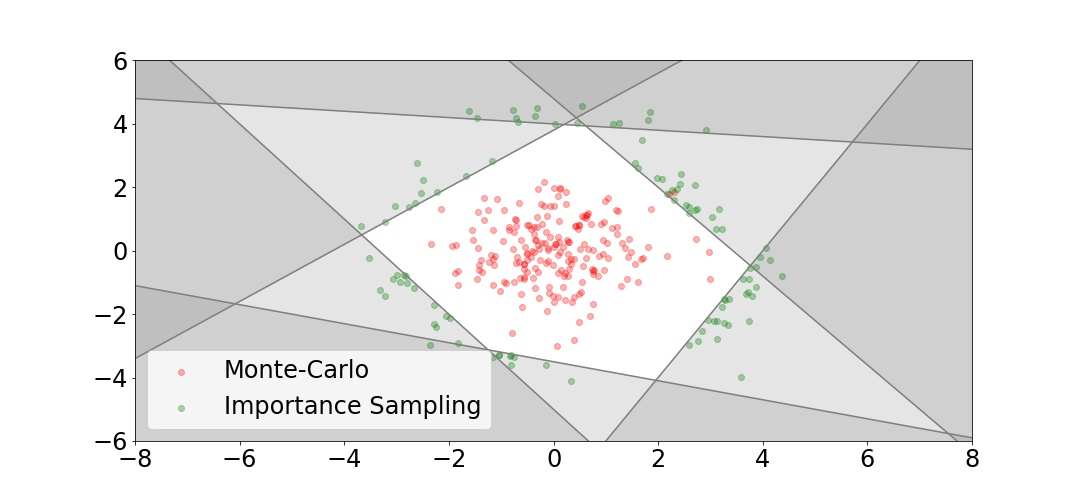
\includegraphics[width=.65\textwidth]{Dissertation/images/sampling/conditioned_vs_MC.jpg}
%     % \vspace{-5mm}
%     \caption{White area stands for generations that do not exceed operating limits. A set of generations leading to at least one constraint violation is in grey. Two or more reliability constraints are not satisfied in dark grey area. Samples from a nominal distribution and the constructed mixture marked in red and green resp. 
%     }
%     \label{fig:00}
%     % \vspace{-5mm}
% \end{figure}

% The estimate is estimated as \begin{align}\label{eq:aloe}
%     {\hat \Pi} = N^{-1}\sum_{i=1}^N \upsilon(p^i)/\upsilon_D(p^i, x^i), \quad p^i \sim D^{x^i},
% \end{align}
% where a distribution mixture $\{D_i\}_{i=1}^K$. The weights $\{x_i\}_{i=1}^K$ define the components of $D$, $p \sim \mathcal{N}(\mu, \Sigma)$ s.t. $p\not\in P$. The main idea is to find weights $x$ such that the estimate has the least variance. The iterative estimation process with updating weights $x^t_i, ~ i=1,\dots K, t=1, \dots k$ is given by
% \begin{align}
%     \hat \Pi = \frac{1}{k}\sum_{t=1}^k \frac{\upsilon(p^t) f(p^t)}{\upsilon_D(p^t, x^t)}, \; p^t \sim \upsilon_D(\cdot, x^t), t\le k \label{eq:emp}
% \end{align}

The last part of the section defines the optimization problem of finding a minimum of the estimate's variance and proves that the problem is convex in mixture weights $x_i$.
The variance minimization problem is
\begin{align}
    \min_x \; & V(x), \; 
    \text{s.t. } x_1 + \dots + x_K = 1, x_k \ge 0, 1\!\le\! k \!\le\! K\label{eq:var-min}
\end{align}
in $x$ for the mixture distribution $\upsilon_D(p,x) = \sum_{i=1}^K x_i \upsilon_i(p)$. %To improve numerical stability one may also add constraints $x_i \ge \varepsilon > 0$ that guarantee that the variance is bounded.
The section concludes with several theorems that establish the convexity of Problem \eqref{eq:var-min}, expression for its gradient, unbiasedness of the resulting estimate and expression for the estimate's variance.
% \begin{theorem}\label{thm:var-convexity}
% Problem~\eqref{eq:var-min} is convex in $x$, and for $x > 0$
% \begin{align*}
%     \nabla V(x) = \int_{\mathbb{R}^n} - f^2 (p)\upsilon^2(p)\upsilon_D^{-2}(p,x) (\upsilon_1(p), \dots, \upsilon_K(p))^\top dp.
% \end{align*} 
% \end{theorem}

% Importantly, the estimation studied is convex: 
% \begin{theorem}\label{thm:unbias}
% $\hat \Pi$ is an unbiased estimate of $\Pi$ if for all $k$, $1\le k \le N$, $x_k > 0$ and $x_k$ is independent of $x^j$ and $p^j$ for~$N\ge j > k\ge 1$.
% \end{theorem}

% Moreover, the variance of $\hat{\Pi}$ is also has the following property:
% \begin{theorem}\label{thm:var}
% Variance of $\hat\Pi$ equals $N^{-2}\sum_{k=1}^N V(x^k)$ if for all $k$ and $j,$ $1\le k < j \le N$, $x_k > 0$ and $x_k$ is independent of $x^j$ and~$p^j$.
% \end{theorem}

Section 3.3 setups the iterative scheme for updating weights $x^t$ using Mirror Descent with Bregman divergence based on negative entropy. The update is:
% \begin{align}\label{eq:md-upd}
%     \!\!x^{k+1} = \argmin\limits_{x\in S}\left\{\eta^k \nabla V(x^k)^\top (x - x^k) + D_\omega(x, x^k)\right\}\!\!,
% \end{align}
% where $S =\{x \ge 0,x_1+\dots+ x_K = 1\}$, a step-size $\eta^k \!>\! 0$, 
% $D_\omega(x, x^k)$ is the Bregman divergence defined for any strongly convex and smooth (distance-generating) function~$\omega$~as
% $
%     D_\omega(x, x^k) = \omega(x) - \{\omega(x^k) + \nabla \omega(x^k)^\top (x^k - x)\}.
% $
% So as the distance generating function is strongly convex and smooth in $x,$ so is the Bregman divergence. When $\omega(x) = \|x\|_2^2/2,$ mirror descent step is the same as in the gradient descent method, $x^{k+1} = x_k - \eta^k \nabla V(x^k)$. However, the negative entropy, $\omega(x) = -\sum_{i=1}^n x_i \log x_i$, is known to be the optimal choice for simplex constrained optimization. For $k\ge 1$ and $1\le i \le K$, solving~Eq.~\eqref{eq:md-upd} in $x$ leads to an update 
\begin{align}
\label{eq:_upd}x^{k+1}_i = x^k_i \frac{\exp(-\eta^k(\nabla V(x^k))_i)}{\sum_{j=1}^K x^k_j \exp(-\eta^k(\nabla V(x^k))_j)}, \eta^k > 0.
\end{align}

Next, the section presents the convergence properties
% \begin{theorem}\label{thm:lan}
%     For any function $V(x)$ that is $M$-Lipschitz in $\ell_1$ norm, i.e. $\|V(x) - V(y)\|_\infty \le M \|x-y\|_1 \forall x,y$, a constant step-size policy $\eta^k = \eta \le 1/M$, and 
%     a sequence $\{x^k\}_{k\ge 1}$ generated by \eqref{eq:md-upd} with $\omega(x) = \sum_{i\le K} x_i\log x_i$, one has
%     \begin{align*}
%         N^{-1}\sum_{i=1}^N (V(x^i)  - V^*) \le 
%         (\log K + (M^2 + \sigma^2) N \eta^2)/(N\eta),
%     \end{align*}
% with $\mathbb{E}_{\upsilon_D}\|g(p,x)- \nabla V(x)\|_\infty^2 \le \sigma^2$, $V_*$ is the optimum of~\eqref{eq:var-min}. 
% \end{theorem}
% To this end, according to Theorem~\ref{thm:lan} 
with the optimal choice of 
$\eta = M^{-1}\sqrt{\log K/(5N)},$ which yields almost dimension independent convergence rate stated in  Theorem~\ref{thm:md-c}. 
\begin{theorem}\label{thm:md-c} Mirror descent with an update~\eqref{eq:_upd} and a step-size policy $\eta^k \!=\! \eta M^{-1}\!\sqrt{(\log K)/N}$,  $\eta \sqrt{(\log K)/N}\!\le\! 1$ yields
\begin{align*}
    \mathbb{V}_{\upsilon_D} (\hat \Pi) = N^{-1}\sum_{k=1}^N V(x^k) < \frac{V^*}{N} +  \left(\frac{M}{\eta}+ \frac{5\eta}{M}\right)\frac{\sqrt{\log K}}{\eta N^{3/2}}, 
\end{align*}
with $M \!= \!\max_{i\le K}\varepsilon^{-2}\Pi_i^2$,  $x\!\ge\! \varepsilon$, $V^*$ be the optimum of~\eqref{eq:var-min}.
\end{theorem}

Compared to the earlier results of~\cite{owen2019importance}, the rate of convergence depends as $O(\sqrt{\log K})$ on the dimension $K$, while earlier results \cite{owen2019importance} claim linear dependence. Thus, the proposed methods results in a substantial acceleration for large-scale problems.

Section 3.4 presents an extensive numerical comparison of the proposed method with state-of-the-art estimation algorithms for the Gaussian polyhedron volume: pmvnorm and ALOE. The most important empirical findings are that there are two simple cases where pmvnorm and ALOE fail. The first one is a degenerate polytope and the second one is just a simple regular polytope with 360 faces that approximates a circle. Both cases are 2 dimensional.

% We consider a regular 2 dimensional polytope with $K$ faces ($K\ge 3$) centered at zero, $
%     P = \{p \in \mathbb{R}^2: \omega_j^\top x \leq \tau, 1\le j \le K\},
% $
% where $\omega_j = (\sin(2\pi j/K), \cos(2 \pi j/K))$. 
% We assume $p\sim\mathcal{N}(0, I_2)$, where $I_2$ is $2\times 2$ identity matrix. The probability $p\not\in P$ rapidly converges to $\exp(-\tau^2/2)$ as $K\to\infty$ \cite{owen2019importance}

% As the second example we consider a degenerate polytope with $K=1500$ faces, where $\omega_1 = (0, 1)$  and $\omega_j = (\xi, -1 - \xi)$, $2\le j \le K$. We take $\xi \sim \mathcal{U}[-\varepsilon, \varepsilon]$ for small $\varepsilon = 10^{-6}$. Note that $\omega_j$ for $j\geq 2$ are almost identical. Hence probability $\Pi$ is quite close to $2\Phi(-\tau)$.
% The results are shown in Figure \ref{fig:01}, showing stability of the proposed algorithm (MD-Var)

% \begin{figure}[t!]
%     \centering
%     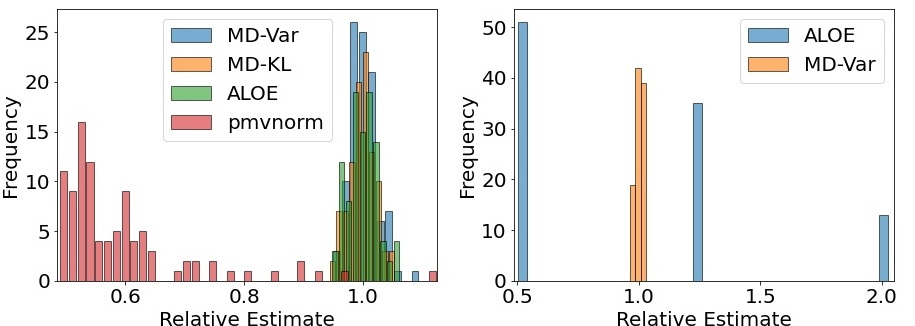
\includegraphics[width=.65\textwidth]{Dissertation/images/sampling/histograms.jpg}
%     %\vspace{-.5mm}
%     %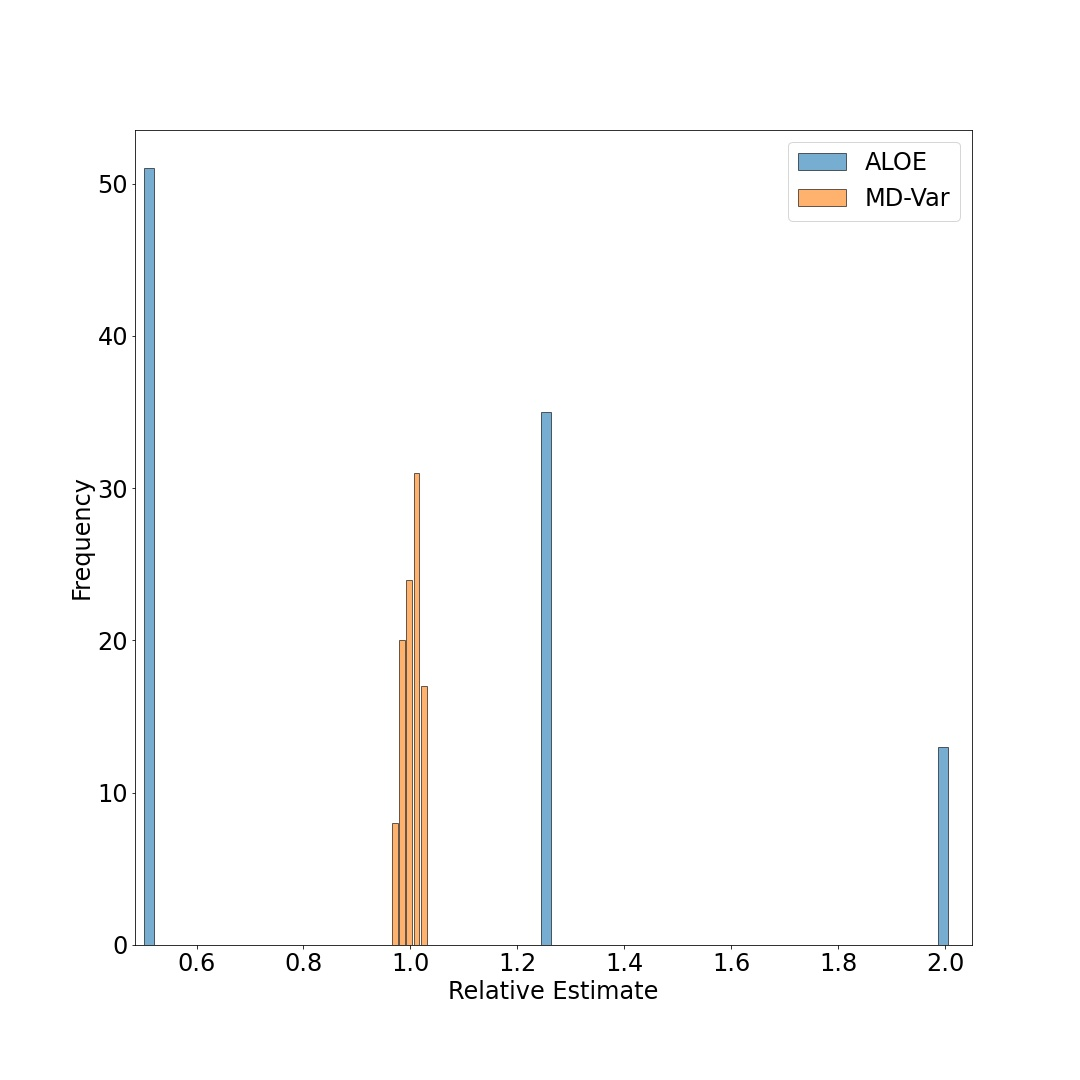
\includegraphics[width=.22\textwidth]{Dissertation/images/sampling/histogram_degenerate.jpg}%\hspace{-3mm}
%     %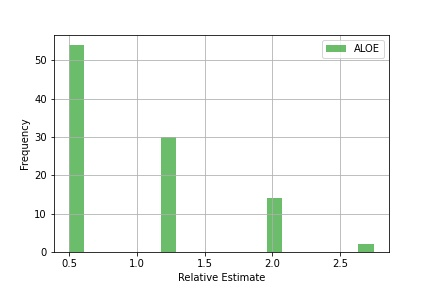
\includegraphics[width=.25\textwidth]{Dissertation/images/sampling/IS_hists_shivering_only_OMC.jpg}
%     \caption{Importance 
%     sampling methods performance on a 2-dimensional (left) regular polytope with $360$ faces; (right) degenerate polytope with $1500$ faces. Overload probabilities are  $\Phi(-6)$ and $2\Phi(-1)$ resp. 
%     }
%     \label{fig:01}
%     % \vspace{-5mm}
% %\end{figure}
% %\begin{figure}[t!]
% %    \centering
%     %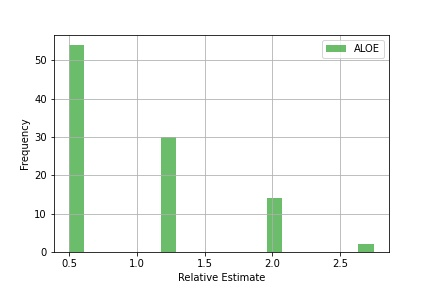
\includegraphics[width=.25\textwidth]{Dissertation/images/sampling/IS_hists_shivering_only_OMC.jpg}
%     %\caption{Importance 
%     %sampling methods performance on a 2-dimensional degenerate polytope with $1500$ faces and overload probability $2\Phi(-1)$.}
%     %\label{fig:degenerate_polytope}
%     %\vspace{-5mm}
% \end{figure}


For power grid test cases, we ran the algorithms on all the test cases accessible through PandaPower~\cite{pandapower.2018}. There were 27 cases with the number of buses varying from 4 to 9241. The proposed methods (MD-Var and MD-KL) took less than two minutes of computational time on a personal laptop for each of them. 
%
Table~\ref{tab:sample-compX} shows the minimal number of samples that are required by the algorithms to achieve \begin{align}    
\Pi/2 \le \hat\Pi \pm s(\hat\Pi) \le 3\Pi/2, \label{eq:tk}\end{align}
where $s(\hat\Pi)$ is the empirical standard deviation of the estimate. This ensures that not only the estimated value, but also its confidence interval is contained in $(\Pi/2, 3\Pi/2)$ and that the sum of the empirical estimate and its standard deviation are close to %of the same order as 
the true probability. 


\begin{table}[ht]
\centering
%\vspace{-4mm}
% \captionsetup{justification=centering}
\caption{Number of samples to satisfy Ineq.~\eqref{eq:tk} 
 for Iceland118}
 \begin{tabular}{|c|c|c|c|c|} 
 \hspace{-2mm}Bound ${\bar\theta}_{ij}$, probability $\Pi$ & MC & ALOE & Pmvnorm & MD-Var\\
 % &&& \cite{genz2020package} & (Section \ref{sampling:nm})\\
 \hline
  \hspace{-2mm}$|{\theta}_{ij}| \le \pi/8$, $\Pi$ = 1.2e-01 & 6.4e+02 & 3.7e+02 & \underline{3.2e+02} & 4.1e+02\\
  \hspace{-2mm}$|{\theta}_{ij}| \le \pi/7$, $\Pi$ = 3.0e-02 & 5.1e+04 & 4.1e+02 & 1.1e+03 & \underline{3.5e+02}\\
  \hspace{-2mm}$|{\theta}_{ij}| \le \pi/6$, $\Pi$ = 2.5e-03  & 6.2e+06 & 4.5e+02 & 6.3e+03 & \underline{3.9e+02} \\
  \hspace{-2mm}$|{\theta}_{ij}| \le \pi/5$, $\Pi$ = 2.6e-05  & 8.9e+10 & 3.3e+02 & 1.4e+04 & \underline{2.1e+02}\\
  \bottomrule
 \end{tabular}
 \vspace{-0mm}\label{tab:sample-compX}
\end{table}


% Table~\ref{tab:emp} shows overload probability estimates and their standard deviations for the algorithms based on $N = 200$ samples on various PandaPower~\cite{pandapower.2018} power grids.


Finally, the chapter concludes. Importance sampling proves invaluable for promptly evaluating the reliability of power grids in real-time scenarios. Our proposed algorithm innovatively creates a mixture distribution tailored to the grid's physics, enhancing accuracy. Through convex optimization, we fine-tune the mixture weights, surpassing existing methods in both precision and speed. This advancement opens doors for its application in optimizing and controlling power grids, promising enhanced efficiency and reliability.

\textbf{The fourth chapter} presents the approach for constructing scenario approximation for DC-OPF assuming additive Gaussian noise for generators. In other words, for linear program with additive Gaussian noise. 

The chapter starts with an introduction in Section 4.1 underscoring the industry need for efficient data-driven SA of Joint Chance Constrained (JCC) optimization problems for modeling optimal, reliable and non conservative generation regimes for high voltage power grids. 
%Next, this Section discusses recent advantages in this field and outlines the main problem: current ways of constructing SA are lead to extremely large linear optimization problems which are challenging to solve. Finally, it outlines the proposed solution - construct a proxy for redundant set of scenario and sample data using ALOE algorithm outside of that region.

Section 4.2 introduces notation and recalls the polyhedron in generation vector $p$ as in Chapter 3. Next, it formulates the JCC optimization problem under consideration:
\begin{equation}\label{eq:JCC-OPF}
    \begin{aligned}
  \min_x & \;\mathbb{E}_{\xi\sim \mathcal{N}(0, \Sigma)} \textit{cost}(x,\xi)\\
   \textit{s. t. }\; & \mathbb{P}_{\xi\sim \mathcal{N}(0, \Sigma)} (x+\xi \in \mathcal{P}) \ge 1 - \eta
   \end{aligned}
\end{equation}

Finally, it presents the SA for this JCC and recalls the number of data samples required to obtain $1-\delta$ reliable solution, i.e., solution of SA that is feasible to original JCC with probability $1-\delta$:
\begin{align}\label{eq:sc-opf}
  \min_x & \; \frac{1}{N} \sum_{t=1}^N \textit{cost}(x,\xi^t)\\
  \textit{s. t. } & \; p^{\min} \le x+\xi^t \le p^{\max}, \; 1\le t \le N\nonumber\\
  & \; |\theta_i(\xi^t) - \theta_j(\xi^t)| \le {\bar \theta}_{ij}, (i, j)\in \mathcal{E}, \; 1\le t \le N\nonumber\\
  & x+\xi^t = B \theta(\xi^t), \; 1\le t \le N\nonumber
\end{align}
The key disadvantage of the scenario approximation \eqref{eq:sc-opf} is the number of constraints induced by adding scenarios $\xi^t$. A classical theory, developed by Calafiore and Campi \cite{calafiore2006scenario}, suggests to include a large number of scenarios $N$. This will allow the solution of \eqref{eq:sc-opf} to be feasible for original problem \eqref{eq:JCC-OPF} with high probability $1 - \delta$. However, the number of required scenarios $N$ is given by $N \geq 2 \left( \frac{\ln{1/\delta}}{\eta} + d + d\frac{\ln{1/\eta}}{\eta} \right)$, where $d$ is the number of control variable in the optimization problem. For example, with $\eta = 10^{-2}, \delta = 10^{-2}$, for  IEEE-57 case one would end up with $6.45 \cdot 10^3$ (6 generators, excluding slack one) constraints which is time- and memory-consuming to solve.

Section 4.3 present the sketch of the proposed approach, formalizes it introduces the redundant region, applies importance sampling. Finally, it presents the theorems that prove the theoretical advantage in number of scenarios in SA.

It starts with the discussion of interrelations between original deterministic feasibility set under probability $\mathcal{P}$, and approximations of JCC feasibility sets. 

The approach follows these steps:

\begin{enumerate}
    \item Construct an inner approximation of the feasibility set.
    \item Generate samples outside this approximation.
    \item Solve the scenario approximation Problem using the generated samples.
\end{enumerate}


First, leveraging the fact that "the probability of a union of events is bounded from below by the maximum of individual event probabilities," we establish a lower bound on the probability of constraint feasibility $\mathbb{P}(x+\xi \in \mathcal{P})$. This allows us to add constraints $x\in \mathcal{P}_{out}$, ensuring that if $x \notin \mathcal{P}_{out}$, then $\mathbb{P}(x+\xi \notin \mathcal{P}) > \eta$. Hence, if the solution $\bar x$ of the scenario approximation with samples from the nominal distribution $\mathcal{N}(0,\Sigma)$ satisfies $\mathbb{P}(x+\xi \in \mathcal{P}) \ge 1-\eta$, adding constraints $x \in \mathcal{P}_{out}$ does not alter $\bar x$.

Second, using the aforementioned bound, we define a polytope $\mathcal{P}{\texttt{in}}(x) = {p: W_{\texttt{in}} \xi \le b_{\texttt{in}}, p = x+\xi}$ around $x$, with $W_{\texttt{in}}$ and $b_{\texttt{in}}$ independent of $x$, which is illustrated in Figure~\ref{fig:10}
%The exact expressions for $W_{\texttt{in}}$ and $b_{\texttt{in}}$ are given in Theorem \ref{thm:20} and illustrated in Figure~\ref{fig:10}.

We demonstrate that for any sample $\xi^t$ and feasible $x$, if $p = x+\xi^t \in \mathcal{P}_{\texttt{in}}(x)$, then $p$ also belongs to the constraint feasibility set $\mathcal{P}$. Thus, scenarios $\xi^t: x+\xi^t \in \mathcal{P}_{\texttt{in}}$ can be excluded from the SA optimization problem  without losing approximation accuracy.

Finally, we sample scenarios outside of the polyhedron $\mathcal{P}_{\texttt{in}}$ using state-of-the-art importance sampling methods \cite{owen2019importance,lukashevich2021power} and solve the Scenario Approximation Problem with the generated samples.
\def\shift{2.7}
\def\shiftt{2.35}
\def\shiftuselesssample{0.3}
\def\shiftusefulsample{1.1}
\begin{figure}
    \centering
        \begin{tikzpicture}[scale=0.75, node distance={15mm}, thick, main/.style = {draw, scale=.9}] 
        %x
        \coordinate (x) at (0, 0);
        \draw (x) circle (1pt);
        \draw (x) ++(0.05, 0.05) node[above right] (tmp) {$x$};
        %x2
        \coordinate (x2) at (0 + \shiftt, 0 - \shiftt);
        \draw (x2) circle (1pt);
        \draw (x2) ++(0.05, 0.05) node[above right] (tmp) {$x^*$};
        %outer guy
        \coordinate (a) at ( 4.755282581475767 , 1.545084971874737 );
        \coordinate (b) at ( 3.061616997868383e-16 , 5.0 );
        \coordinate (c) at ( -4.755282581475767 , 1.5450849718747375 );
        \coordinate (d) at ( -2.9389262614623664 , -4.045084971874736 );
        \coordinate (e) at ( 2.9389262614623646 , -4.045084971874738 );
        %linking outer guy
        \draw (a) -- (b);
        \draw (b) -- (c);
        \draw (c) -- (d);
        \draw (d) -- (e);
        \draw (e) -- (a);
        %annotating outer guy
        \draw
        (a) ++(0.1, 0.01) node[above] (tmp) {$\mathcal{P}$};
        %(tmp.west) -- (PO);
        
        %green guy
        \coordinate (ag) at ( 3.804226065180614 , 1.2360679774997896 );
        \coordinate (bg) at ( 2.4492935982947064e-16 , 4.0 );
        \coordinate (cg) at ( -3.804226065180614 , 1.23606797749979 );
        \coordinate (dg) at ( -2.351141009169893 , -3.2360679774997894 );
        \coordinate (eg) at ( 2.3511410091698917 , -3.2360679774997902 );
        %linking green guy
        \draw [olive] (ag) -- (bg);
        \draw [olive] (bg) -- (cg);
        \draw [olive] (cg) -- (dg);
        \draw [olive] (dg) -- (eg);
        \draw [olive] (eg) -- (ag);
        %annotating green guy
        \draw
        (bg) ++(0.1, 0.01) node[below, olive] (tmp) {$\mathcal{P}_{out}$};
        %(tmp.west) -- (PO);
        
        %red guy
        \coordinate (ar) at ( 0.9510565162951535 , 0.3090169943749474 );
        \coordinate (br) at ( 6.123233995736766e-17 , 1.0 );
        \coordinate (cr) at ( -0.9510565162951535 , 0.3090169943749475 );
        \coordinate (dr) at ( -0.5877852522924732 , -0.8090169943749473 );
        \coordinate (er) at ( 0.5877852522924729 , -0.8090169943749476 );
        %linking red guy
        \draw [red] (ar) -- (br);
        \draw [red] (br) -- (cr);
        \draw [red] (cr) -- (dr);
        \draw [red] (dr) -- (er);
        \draw [red] (er) -- (ar);
        %annotating red guy
        \draw
        (br) ++(1em, .1em) node[above right, red] (tmp) {$\mathcal{P}_{\texttt{in}}(x)$};
        %(tmp.west) -- (PO);
        
        %red guy2
        \coordinate (ar2) at ( 0.9510565162951535 + \shiftt , 0.3090169943749474 - \shiftt);
        \coordinate (br2) at ( 6.123233995736766e-17 + \shiftt , 1.0  - \shiftt);
        \coordinate (cr2) at ( -0.9510565162951535  + \shiftt, 0.3090169943749475  - \shiftt);
        \coordinate (dr2) at ( -0.5877852522924732 + \shiftt, -0.8090169943749473 - \shiftt);
        \coordinate (er2) at ( 0.5877852522924729 + \shiftt, -0.8090169943749476  - \shiftt);
        %linking red guy
        \draw [red] (ar2) -- (br2);
        \draw [red] (br2) -- (cr2);
        \draw [red] (cr2) -- (dr2);
        \draw [red] (dr2) -- (er2);
        \draw [red] (er2) -- (ar2);
        %annotating red guy
        \draw
        (br2) ++(1em, .1em) node[above, red] (tmp) {$\mathcal{P}_{\texttt{in}}(x^*)$};
        %(tmp.west) -- (PO);
        
        %Upper \Delta_i
        \coordinate (b_) at (1, 5.7265);
        \draw
        (b_) node[above right] (tmp) {$\Delta_i$};
        %(tmp.west) -- (PO);
        \coordinate (bg_) at (1.5, 5.0898);
        \draw [dashed] (b) -- (b_);
        \draw [dashed] (bg) -- (bg_);
        \draw [thick, black, -latex'] (b_) -- (bg_);
        \draw [thick, black, -latex'] (bg_) -- (b_);
        
        %Inner \Delta_i
        \coordinate (br_) at (-1.5, -0.0898137920080413);
        \draw
        (br_) node[above left] (tmp) {$\Delta_i$};
        %(tmp.west) -- (PO);
        \coordinate (x0_) at (-1.0, -0.7265425280053608);%x!
        \draw [dashed] (br) -- (br_);
        \draw [dashed] (x) -- (x0_);
        \draw [thick, black, -latex'] (br_) -- (x0_);
        \draw [thick, black, -latex'] (x0_) -- (br_);
        
        %Inner \Delta_i 2
        \coordinate (br_2) at (-1.5 + \shiftt, -0.0898137920080413 - \shiftt);
        \draw
        (br_2) node[above left] (tmp) {$\Delta_i$};
        %(tmp.west) -- (PO);
        \coordinate (x0_2) at (-1.0 + \shiftt, -0.7265425280053608-  \shiftt);%x!
        \draw [dashed] (br2) -- (br_2);
        \draw [dashed] (x2) -- (x0_2);
        \draw [thick, black, -latex'] (br_2) -- (x0_2);
        \draw [thick, black, -latex'] (x0_2) -- (br_2);
        
        % Samples
        %% Useless
        \coordinate (xu_1) at (\shiftt + \shiftusefulsample * 0.1, -\shiftt - 3.5*\shiftuselesssample);
        \draw [teal] (xu_1) circle (1pt);
        \coordinate (xu_2) at (\shiftt + \shiftusefulsample, -\shiftt + \shiftusefulsample * 0.5);
        \draw [teal] (xu_2) circle (1pt);
        \coordinate (xu_3) at (\shiftt - \shiftusefulsample * 0.2, -\shiftt + \shiftusefulsample);
        \draw [teal] (xu_3) circle (1pt);
        \coordinate (xu_4) at (\shiftt + \shiftusefulsample * 0.7, -\shiftt - \shiftusefulsample);
        \draw [teal] (xu_4) circle (1pt);
        \end{tikzpicture}  
\caption{We consider a deterministic feasibility set $\mathcal{P}$ and derive a polytope $\mathcal{P}_{out}$ inside of it so that no optimal solution $x^*$ of Prob.~ \eqref{eq:JCC-OPF} belongs to $\mathcal{P}\setminus \mathcal{P}_{out}$. The polytope $\mathcal{P}_{\texttt{in}}(x)$ depicts the distances between the planes of $\mathcal{P}$ and $\mathcal{P}_{out}$ for each $x$.
%The polytope $\mathcal{P}_{\texttt{in}}$, defined in terms of noise $\xi$ only, $.
Samples of uncertainty outside $\mathcal{P}_{\texttt{in}}(0)$ are used to determine optimal solution using importance sampling.}
  \label{fig:10}
  %\vspace
\end{figure}

The inner approximation can be obtained by the Boole-Frechet inequality:
\begin{align*}
  \mathbb{P}&(p\in \mathcal{P}) = 
  \mathbb{P}(p: Wp \le b) =\\
  & 1 - \max_{1\le i\le J}\mathbb{P}\left(p: \omega_i^\top p > b_i\right).
\end{align*}
Further, taking into account Gaussianity and considering the case when there exists a plane that exceed the probability $\eta$, one can obtain the following expression for the outer approximation of the JCC - $\mathcal{P}_{out}$:

\begin{align}\label{eq:05}
  P_{out} = \left\{x: \omega_i^\top x \le b_i - \Delta_i, 1\leq i\leq J\right\},
\end{align}

where $\Delta_i = \|\Sigma^{1/2}\omega_i\|_2 \Phi^{-1}(1-\eta)$, $\eta \le 1/2$.

% For this outer JCC approximation set an important theorem is stated and proved. This theorem proves that the outer approximation is also satisfied for a solution of original JCC problem:
% \begin{theorem}\label{thm:10}
%   The joint chance-constrained optimal power flow problem~ \eqref{eq:JCC-OPF} has the same set of optimal solutions as 
%   \begin{align}\label{eq:JCC-OPF-Ad}
%   \min_x & \;\mathbb{E}_{\xi\sim \mathcal{N}(0, \Sigma)} \textit{cost}(x,\xi)\\
%    \textit{s. t. }\; & \mathbb{P}_{\xi\sim \mathcal{N}(0, \Sigma)} (x+\xi \in \mathcal{P}) \ge 1 - \eta, 0 < \eta \le 1/2,\nonumber\\
%    & \; x\in \mathcal{P}_{out}\nonumber 
% \end{align}
% \end{theorem}

% It is also important to prove that for the SA without including $\mathcal{P}_{out}$ the same logic applies:
% \begin{theorem}\label{thm:20}
% Any solution of the Scenario approximation problem~ \eqref{eq:sc-opf} that is feasible for the Chance-constrained OPF problem~ \eqref{eq:JCC-OPF} is also a solution of 
% %\newpage
% %\begin{align}\label{eq:30}
The Scenario Approximation is given as
\begin{subequations}
\label{eq:Fin}
  \begin{equation}
  \min_x \; \textit{cost}(x)\nonumber
  \end{equation}
  \begin{equation}
  \hspace{-20mm}\textit{s. t. }\;\; p^{\min} \le x+\xi^t \le p^{\max}, \; 1\le t \le N\label{eq:Fin-a}
  \end{equation}
  \begin{equation}
   \hspace{11mm} |\theta_i(\xi^t) - \theta_j(\xi^t)| \le {\bar \theta}_{ij}, (i, j)\in \mathcal{E}, \; 1\le t \le N\label{eq:Fin-b}
  \end{equation}
  \begin{equation}
  \hspace{-19mm} x+\xi^t = B \theta(\xi^t), \; 1\le t \le N\label{eq:Fin-c}
  \end{equation}
  \begin{equation}
  \hspace{-50mm} x\in \mathcal{P}_{out} \label{eq:Fin-d}
  \end{equation}
\end{subequations} 
% \end{theorem}

Recall the standard fundamental assumption that ensures the correctness of theorems that state the lower bound for required number of scenarios from~\cite{calafiore2006scenario}:
\begin{assumption}\label{asmp:10}
Assume that for all possible uncertainty realizations $\xi^1, \dots, \xi^N$, the optimization problem \eqref{eq:Fin} is either infeasible or, if feasible, it attains a unique optimal solution.
\end{assumption}

This assumption allows to proof the main theorem of this chapter. The following statement shows that the number of scenarios required is reduced by the measure of $\mathcal{P}_{in}$ which is denoted by $\pi$:
\begin{theorem}\label{thm:40}
Let $\bar x_N$ be a unique solution of the Scenario optimization Problem~\eqref{eq:Fin} with $N$ i.i.d. samples, so that none of the samples belong to $\mathcal{P}_{\texttt{in}}$. Moreover, assume that for any $N$ the assumption \ref{asmp:10} is fulfilled. Then for any $\delta \in (0,1)$ and any~$\eta \in (0, 1/2]$, $\bar x_N$ is also a solution for the Chance-constrained optimal power flow Problem~\eqref{eq:JCC-OPF} with probability at least $1-\delta$ if 
\begin{align*}
  N \ge \left\lceil 2\frac{(1-\pi)\ln \frac{1}{\delta}}{\eta} + 2d + 2d (1-\pi) \frac{\ln\frac{2(1-\pi)}{\eta}}{\eta} \right\rceil, 
\end{align*} 
where $d$ is a dimension of the space of controllable generators, and $\pi$ is the probability of a random scenario $\xi\sim \mathcal{N}(0, \Sigma)$ to belong to $\mathcal{P}_{\texttt{in}}$, and $\pi < 1$. 
\end{theorem}

Unfortunately, there isn't a precise and efficient algorithm for sampling from a Gaussian distribution outside a convex polytope \cite{khachiyan1993complexity}. However, the ALOE algorithm \cite{owen2019importance, lukashevich2021power} provides a sophisticated method for approximating the desired distribution by sampling from a mixture of distributions.

We focus on Gaussian fluctuations of power injections, $\xi \sim \mathcal{N}(0, \Sigma)$, with known covariance matrix $\Sigma \in \mathbb{R}^{n \times n}$. Our aim is to sample scenarios outside $\mathcal{P}_{\texttt{in}}$, ensuring that the sampling distribution closely approximates the conditional Gaussian distribution $\xi \sim \mathcal{N}(0, \Sigma) \textit{s.t. } \xi \not\in \mathcal{P}_{\texttt{in}}$.

We use the same algorithm for sampling from distribution $D$ as in previous chapter:
\begin{align}\label{eq:q_d}
  D = \sum_{i=1}^J \alpha_i D_i, \; & \alpha_i \ge 0, \sum_{i=1}^J \alpha_i = 1,\nonumber \\
  & \alpha_i \propto \Phi(-\Delta_i/\|\Sigma^{1/2}\omega_i\|_2),
\end{align}
where $\Phi$ is a CDF of the standard normal distribution. Let $q_D(\xi)$ be a PDF of distribution $D$, then Theorem~\ref{thm:50} established a maximal ratio of the conditional Gaussian density~$\xi\sim\mathcal{N}(0, \Sigma) \textit{s. t. } \xi\not\in\mathcal{P}_{\texttt{in}}$ and~$q_D(\xi)$.

It is important to formalize the inaccuracy of modeling the Gaussian conditioned on a polyhedron's complement with out-of-plane Gaussian mixtures.
Let $q_D(\xi)$ be a PDF of distribution $D$, then Theorem~\ref{thm:50} established a maximal ratio of the conditional Gaussian density~$\xi\sim\mathcal{N}(0, \Sigma) \textit{s. t. } \xi\not\in\mathcal{P}_{\texttt{in}}$ and~$q_D(\xi)$. 

\begin{theorem}\label{thm:50}
Let $\nu(\xi)$, $q_D(\xi)$ be PDFs  of $\xi\sim\mathcal{N}(0, \Sigma) \textit{s. t. } \xi\not\in\mathcal{P}_{\texttt{in}}$, and a mixture density (see Eq.~\eqref{eq:q_d}), resp. Then for any $\xi\not\in\mathcal{P}_{\texttt{in}}$, we have
\begin{align}\label{eq:M}
  \nu(\xi) \le M q_D(\xi),  
  M = \frac{\sum_{i\le J} \Phi(-\Delta_i/\|\Sigma^{1/2}\omega_i\|_2)
  }{\max_{i\le J}\Phi(-\Delta_i/\|\Sigma^{1/2}\omega_i\|_2)}, 
\end{align}
where $D$ and $\alpha_i$ are given in Eq.~\eqref{eq:q_d}.
\end{theorem}

In particular, we solve the following optimization problem instead of Problem~\eqref{eq:sc-opf}: 
\begin{subequations} 
\label{eq:FinA}
  \begin{equation}
  \min_x \; \textit{cost}(x)\nonumber
  \end{equation}
  \begin{equation}
  \hspace{-20mm}\textit{s. t. }\;\; p^{\min} \le x+\xi^t \le p^{\max}, \; 1\le t \le N\label{eq:FinA-a}
  \end{equation}
  \begin{equation}
   \hspace{11mm} |\theta_i(\xi^t) - \theta_j(\xi^t)| \le {\bar \theta}_{ij}, (i, j)\in \mathcal{E}, \; 1\le t \le N\label{eq:FinA-b}
  \end{equation}
  \begin{equation}
  \hspace{-19mm} x+\xi^t = B \theta(\xi^t), \; 1\le t \le N\label{eq:FinA-c}
  \end{equation}
  \begin{equation}
  \hspace{-50mm} x\in \mathcal{P}_{out} \label{eq:FinA-d}
  \end{equation}
  \begin{equation}
  \hspace{-32mm} \xi^1, \xi^2, \dots, \xi^N\sim D \label{eq:FinA-e},
  \end{equation}
\end{subequations}

Finishing the practical implementation, the next theorem shows the advantage in number of samples required to obtain reliable SA solution:

\begin{theorem}\label{thm:80}
Let $\bar x_N$ be a unique solution of the Scenario optimization Problem~\eqref{eq:FinA} with $N$ i.i.d. samples follow distribution $D$. Moreover, assume that for any $N$ the assumption \ref{asmp:10} is fulfilled. Then for any $\delta \in (0,1)$ and any~$\eta \in (0, 1/2]$, $\bar x_N$ is also a solution for the chance-constrained optimal power flow Problem~\eqref{eq:JCC-OPF} with probability at least $1-\delta$ if 
\begin{align*}
  N \ge \left\lceil 2M\frac{(1-\pi)\ln \frac{1}{\delta}}{\eta} + 2d + 2d M(1-\pi) \frac{\ln\frac{2M(1-\pi)}{\eta}}{\eta} \right\rceil, 
\end{align*} 
where $d$ is a dimension of the problem and $\pi$ is a probability of a random scenario $\xi$ to belong to $\mathcal{P}_{\texttt{in}}$, $\pi < 1$, and constant $M$ is defined by Theorem~\ref{thm:50}.
\end{theorem}

% The Section 5.4 presents the numerical comparison of the proposed approach with classical Monte-Carlo based SA. The core of this section is the experimental protocol. The methods are compared based on the estimated solution reliability $1-\hat{\delta}$, i.e., the probability that the SA's solution is feasible to the original JCC. The procedure is summarized in Algorithm \ref{alg:estimate_delta}.
% \begin{algorithm}[ht]
% \SetKwInOut{Input}{input}
% \SetKwRepeat{Do}{do}{while}
% % \SetKwInOut{Output}{output}
% \caption{Reliability $1-\hat{\delta}$ -- an empirical estimate}\label{alg:estimate_delta}
% \Input{$L$ -- number of trials, DC-OPF problem parameters, $\eta$ -- confidence level, $N_0$ -- initial size of scenario approximation, $N_{\max}$ -- maximal size of scenario approximation}
% $N \gets N_0$\;
% $\hat{ \boldsymbol \delta}$ -- storage for $\hat{\delta}_N$\;
% \Do{$N \leq N_{\max}$}
% {
%      $C_N \gets 0$ -- feasibility counter\;
%      $l \gets 1$\;
%     \Do{$l \leq L$}{
%         Obtain $(x^*_N)_l$ -- scenario approximation with $N$ samples (using SA-IS or SA) \;
%         Estimate constraint satisfaction probability $(\hat{\mathbb{P}}_N)_l$ using Monte Carlo samples.\; \label{alg:estimate_delta:phat_N_l}\;
%         \uIf{$(\hat{\mathbb{P}}_N)_l \geq 1 - \eta$}{
%             $C_N \gets C_N +1$
%         }
%         }
%     $1-\hat{\delta}_N \gets C_N / L$ -- fraction of trials turned out to be feasible \;
%     Append $\hat{\delta}_N$ to $\hat{ \boldsymbol \delta}$ \;
%     $n  \gets n + N_{\max}/ 10$\;
% }
% \Return $\hat{ \boldsymbol \delta}$
% \end{algorithm}

The results of comparison are presented in Table \ref{tab:summary_results}. Additionally, the reliability analysis of approximations' solutions is presented in Figures \ref{fig:spreads}, \ref{fig:empiricals}, the latter illustrates empirical reliability ($1-\hat{\delta}$) and the former illustrates the spread of constraint feasibility $(\hat{\mathbb{P}}_N)_l$ for CC-OPF ($1-\eta =.99$) for IEEE 300 bus and IEEE 118 bus systems. The three cases correspond to samples in CC-OPF being drawn by SA, SA-IS and SA-O. The empirical estimates are computed with $L = 100$ optimization instances (for $1-\hat{\delta}$), and $N_{MC}=10^4$ Monte-Carlo samples for each instance to determine constraint validation (for box-plot of $(\hat{\mathbb{P}}_N)_l$). 
Colored boxes stands for the 25\% -- 75\% interquantile range (IQR). Diamonds shows samples outside of the $\pm 1.5*\text{IQR}$. 
Note that both in reliability, and the IRQ of constraint feasibility, SA-IS requires much less number of samples compared to SA or~SA-O. Finally, the execution time of the preprocessing step comparison is visualized in Figure \ref{fig:profile_generate_samples}. On the right Figure, vertical dashed lines indicate number of samples that are sufficient to reach $1-\hat{\delta}=0.99$ reliability level for $\eta=0.05$, see Table \ref{tab:summary_results}. Horizontal dot-dashed lines demonstrate the amount of time spent on average over 15 runs. From this figure, one can observe that ALOE is a more time consuming procedure. However, one can observe that the time required to solve scenario approximations together with preprocessing does not differ significantly for IS-SA and SA -- see Figure \ref{fig:profile_scenario_approx}. The latter figure also shows that the computational time required to obtain the same reliability level is five times less for SA-IS (the number of samples are taken from Table \ref{tab:summary_results}, case IEEE-30, $\eta=0.05$.)

\begin{landscape}
\begin{table*}[t]
\caption{Number of SA-IS and SA samples required to reach reliability level $1-\hat{\delta} = 0.99$ in CC-OPF with confidence threshold $1-\eta$. The number of scenarios required for target reliability were obtained empirically, iterating over a predefined grid for $N$ with the step of $10$.
    The confidence threshold $1-\eta$ is estimated using Monte Carlo samples (out of sample) and empirical reliability is computed by averaging over $L=100$ independent CC-OPF problem instances. The costs of solutions obtained are depicted alongside with the corresponding costs of deterministic DC-OPF solution. It is clear that SA-IS requires much less samples compared to SA, while maintaning the same reliability of the solution.}
    \centering
        \begin{tabular}{|lrrll|rll|l|}
        \toprule
           Case &  $\eta$ &  SA No &  SA Cost &   SA $(\mathbb{P}_N)$ &  IS-SA No & IS-SA Cost & IS-SA $(\mathbb{P}_N)$ & DC-OPF Cost \\
        \midrule
         grid30 &    0.05 &    160 & 5.89e+03 & 9.82e-01$\pm$7.09e-03 &        \textbf{60} &   5.87e+03 &  9.80e-01$\pm$8.86e-03 &    5.67e+03 \\
         grid57 &    0.05 &    210 & 2.52e+04 & 9.78e-01$\pm$8.95e-03 &       \textbf{160} &   2.52e+04 &  9.89e-01$\pm$7.71e-03 &    2.50e+04 \\
        grid118 &    0.05 &   1300 & 8.72e+04 & 9.68e-01$\pm$4.18e-03 &      \textbf{1050} &   8.72e+04 &  9.68e-01$\pm$4.16e-03 &    8.48e+04 \\
        grid300 &    0.05 &   1550 & 4.72e+05 & 9.63e-01$\pm$4.36e-03 &      \textbf{1250} &   4.72e+05 &  9.62e-01$\pm$3.97e-03 &    4.71e+05 \\
        \midrule
         grid30 &    0.01 &    800 & 5.94e+03 & 9.96e-01$\pm$1.83e-03 &       \textbf{300} &   5.96e+03 &  9.99e-01$\pm$6.57e-04 &    5.67e+03 \\
         grid57 &    0.01 &   1300 & 2.52e+04 & 9.96e-01$\pm$1.55e-03 &       \textbf{300} &   2.53e+04 &  9.97e-01$\pm$1.88e-03 &    2.50e+04 \\
        grid118 &    0.01 &   6000 & 8.74e+04 & 9.93e-01$\pm$1.16e-03 &      \textbf{3600} &   8.74e+04 &  9.94e-01$\pm$9.11e-04 &    8.48e+04 \\
        grid300 &    0.01 &   9000 & 4.72e+05 & 9.93e-01$\pm$8.42e-04 &      \textbf{4500} &   4.72e+05 &  9.92e-01$\pm$9.53e-04 &    4.71e+05 \\
        \bottomrule
        \end{tabular}
    \label{tab:summary_results}
\end{table*}
\end{landscape}
\begin{figure*}[hbt]
\centering
\begin{subfigure}{.8\textwidth}
  \centering
  % include first image
  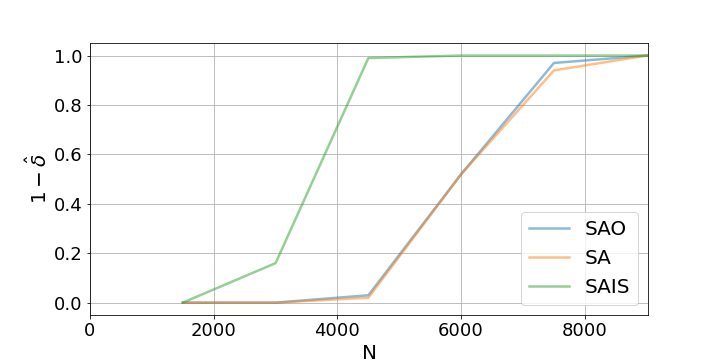
\includegraphics[width=0.99\linewidth]{Dissertation/images/dc_stochastic_approx/case300/1_beta_N_12000_eta_001.png}~~~~~~\hfill
  \caption{IEEE 300 bus system.}
  \label{fig:ieee300reliability}
\end{subfigure}

\begin{subfigure}{.8\textwidth}
  \centering
  % include first image
  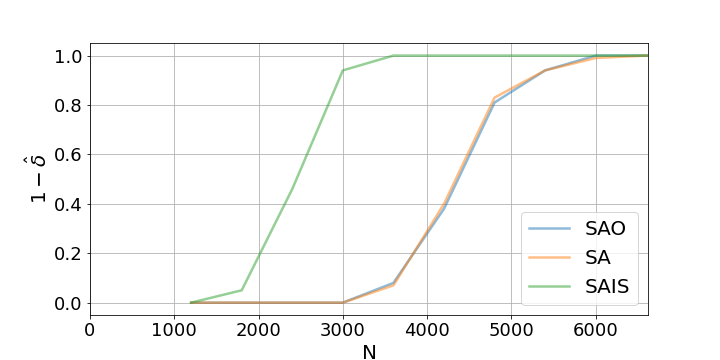
\includegraphics[width=0.99\linewidth]{Dissertation/images/dc_stochastic_approx/ieee118/1_beta_N_7800_eta_001.png}~~~~~~\hfill
  \caption{IEEE 118 bus system.}
  \label{fig:ieee118reliability}
\end{subfigure}
\caption{Empirical reliability ($1-\hat{\delta}$) versus number of samples in \\CC-OPF ($N$).}
\label{fig:empiricals}
\end{figure*}

\begin{figure*}[hbt]
\centering
\begin{subfigure}{.8\textwidth}
  \centering
  % include second image
  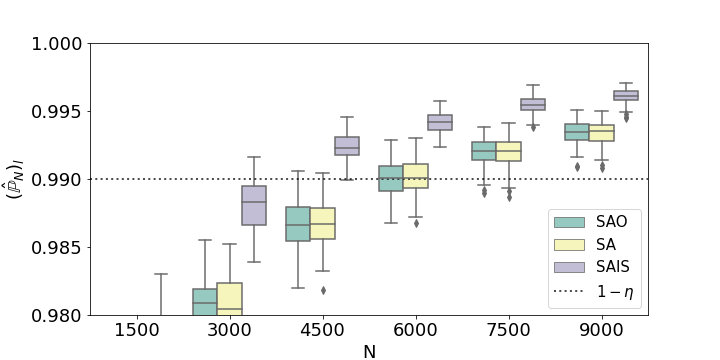
\includegraphics[width=0.99\linewidth]{Dissertation/images/dc_stochastic_approx/case300/boxplot_J_N_9000_eta_001.png}
  \caption{IEEE 300 bus system.}
  \label{fig:ieee300conservatism}
\end{subfigure}

\begin{subfigure}{.8\textwidth}
  \centering
  % include second image
  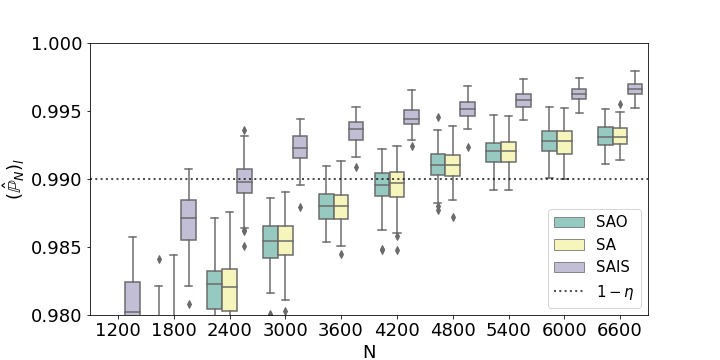
\includegraphics[width=0.99\linewidth]{Dissertation/images/dc_stochastic_approx/ieee118/boxplot_J_N_6600_eta_001.png}
  \caption{IEEE 118 bus system.}
  \label{fig:ieee118conservatism}
\end{subfigure}
\caption{Spread of probability of constraint feasibility ($(\hat{\mathbb{P}}_N)_l$) versus number of samples in CC-OPF ($N$).}
\label{fig:spreads}
\end{figure*}

\begin{figure*}[hbt]
\centering
\begin{subfigure}{.8\textwidth}
  \centering
  % include first image
  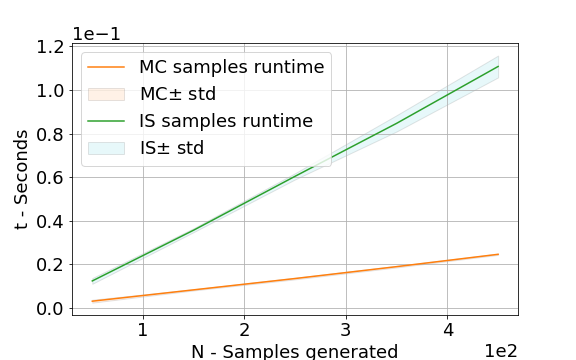
\includegraphics[width=0.9\linewidth]{Dissertation/images/dc_stochastic_approx/profiling_samplig.png}~~~~~~\hfill
  \caption{Sample generation.}
  \label{fig:profile_generate_samples}
\end{subfigure}
\begin{subfigure}{.8\textwidth}
  \centering
  % include second image
  \hspace{-10mm}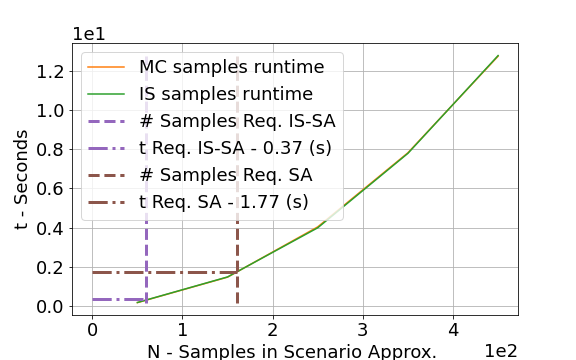
\includegraphics[width=0.9\linewidth]{Dissertation/images/dc_stochastic_approx/profiling_approx_sol.png}
  \caption{Samples preparation, assembling scenario approximation and solving the latter, formed for different $N$.}
  \label{fig:profile_scenario_approx}
\end{subfigure}
\caption{Computational time required to complete prepocessing step \ref{fig:profile_generate_samples} and solve corresponding scenario approximations \ref{fig:profile_scenario_approx} for IEEE-30 case. }
\label{fig:profiling}
\end{figure*}
The experiments were conducted on power system test cases and indicate the robustness and higher data efficiency of the proposed approach.

Finally, the Chapter concludes. In this chapter, we explored scenario approximation for chance-constrained optimal power flow, demonstrating that importance sampling enhances accuracy and reduces numerical complexity for stochastic OPF.
Our theoretical analysis highlights the advantages of using violative samples. Numerical experiments show a significant reduction in sample size needed for high reliability. This approach can also be extended to automated real-time control of bulk power systems.

\textbf{The fifth chapter} presents a generalization for power grid with dynamics. The whole approached as called A-priori Reduced Scenario Approximation (AR-SA). Here the uncertainty is a total power mismatch between generation and demand which is a sum of different distributions included Weibull (wind), Beta (solar) and others. It is worth mentioning that here the uncertainty is multiplicative in contrast to the of additive one from the previous chapter.

Section 5.1 presents the whole approach which is compactly summarized in Figure \ref{fig:workflow}. We compare the performance of AR-SA with other reduction techniques such as Fast Forward, Simultaneous Backward, and K-Means methods on Grid6-WW, Washington-14, and IEEE-30 grids.

\begin{figure}
    \centering
    \hspace{-2mm}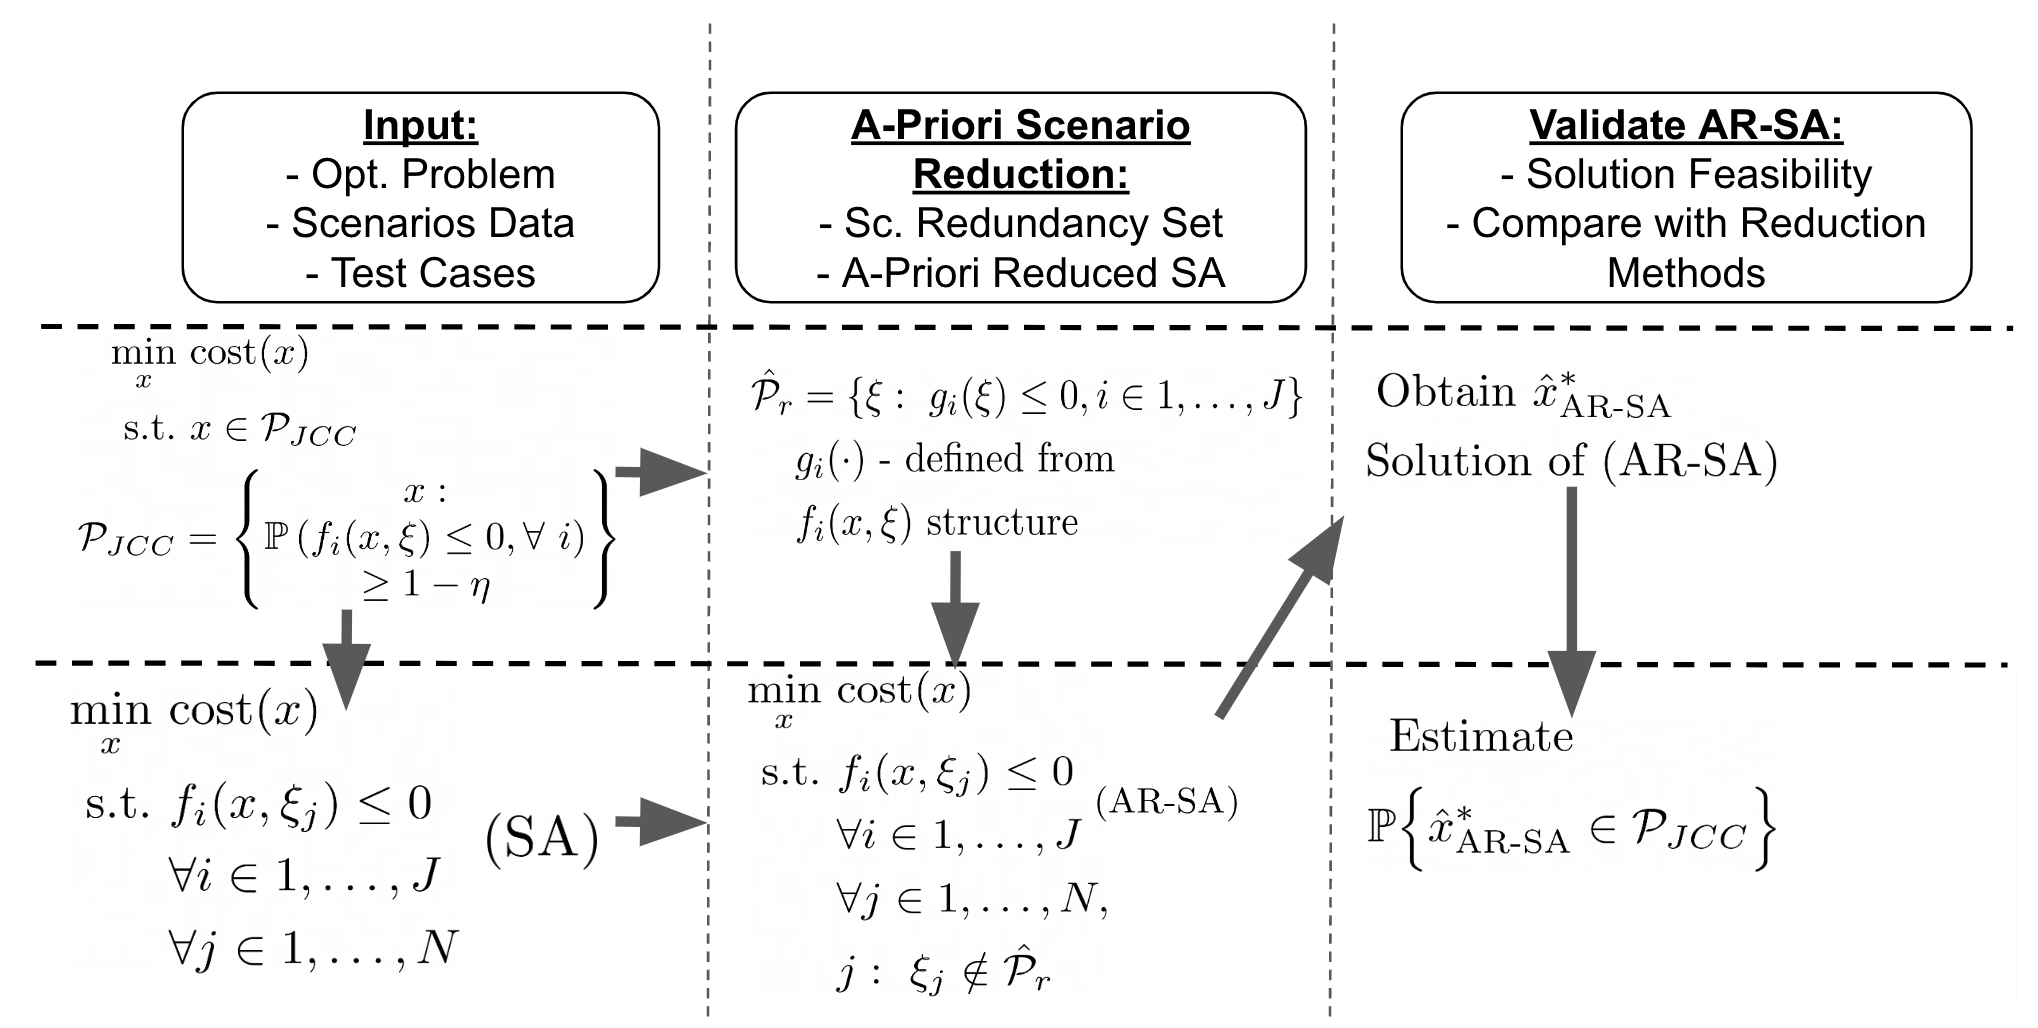
\includegraphics[width=1.\textwidth]{Dissertation/images/dynamic//scheme.png}
    \caption{AR-SA workflow.}
    \label{fig:workflow}
    \vspace{-1mm}
\end{figure}


Section 5.2 recalls the DC-OPF problem and discusses the source of uncertainty and Automated Generation Control (AGC) algorithm to balance the generation-demand mismatch. The AGC recourse adjusts the generation to a new setpoint $p^{t+1} = p^t + \alpha \xi^t$ \cite{roald2017chance,baros2021examining,mezghani2020stochastic} with $p^t \in \mathbb{R}^{n_g}$, $\alpha \in \mathbb{R}^{n_g}$, and $\xi^t \in \mathbb{R}$ representing the \emph{total} demand-generation imbalance.
The total system imbalance $\xi^{t}$ results from the combined power fluctuations due to renewable generation intermittency, demand instability, and intra-day electricity trading. Specifically, for a power system with nodes $\mathcal{B}$, the imbalance is given by $\xi^t = \sum_{b \in \mathcal{B}} (\xi_b^d)^t - (\xi_b^g)^t$, where $(\xi_b^d)^t$ and $(\xi_b^g)^t$ are random variables representing fluctuations in demand and generation at bus $b$ at time $t$, respectively. These random variables follow different distributions depending on their sources. For example, if bus $b$ has a PV generator, $(\xi_b^g)^t$ follows a beta distribution \cite{wang2010probabilistic}. For wind farms, the wind speed follows a Weibull distribution, although power output can vary among turbines \cite{dhople2012framework}. However, $\xi^t$, as the sum of random variables, follows a Gaussian distribution due to the Lyapunov or Lindeberg-Feller Central Limit Theorem \cite{scholz2011central}, \cite{rouaud2013probability, draper2021practical}.

We validated this Gaussian assumption by applying the Shapiro-Wilk normality test \cite{shapiro1965analysis} to the time series of load-renewable generation imbalance estimated from RTS-GLMC data \cite{barrows2019ieee}. This project includes time series data for demand, hydro, rooftop PV, PV, and wind farm generations. The Shapiro-Wilk test indicated that, at a significance level of $\alpha=0.05$, the null hypothesis $H_0$ (the generation-demand imbalance is normally distributed) was rejected only for August and November. Therefore, the assumption that $\xi^t$ is Gaussian is valid.
We further consider the stacked temporal uncertainty vector $\xi = (\xi^1, \dots, \xi^T) \sim \mathcal{N}(\mu, \Sigma)$, with $\Sigma$ modeling temporal correlations.

Section 5.3 ensures that AGC keeps the system balances by checking sequential timestamps and power balance.

Section 5.4 formalizes the JCC formulation for multistep DC-OPF with AGC:
\begin{align}
        & \hspace{32mm} \min_{p^t, \alpha} \mathbb{E} \sum_{t=1}^T c(p^t) \label{eq:optimal_control}, \qquad \texttt{s.t.:} 
        \\ 
        & \; \mathbb{P} 
        \begin{pmatrix}
                Wp^t \leq b, p^t = p^{t-1} + \alpha\xi^t, |p_k^t - p_k^{t-1}| \leq R_k,\\
                 1 \leq k \leq n_g, ~1\leq t \leq T
        \end{pmatrix} \geq 1 - \eta.\nonumber
\end{align}
where $\eta\in (0, 1/2]$, $\mathbb{P}$ is a joint measure induced by the uncertainty distribution, and $\alpha \in \mathbb{R}^{n_g}$ is participation factors.

A compact statement of the Problem \eqref{eq:optimal_control} is:
%assuming no uncertainty for $t = 0$:
\vspace{-3mm}
\[\min_{p^t, \alpha} \mathbb{E} \sum_{t=1}^T c(p^t) \]
\vspace{-3mm}
\begin{equation}
    \begin{aligned}
        \!\!\texttt{s.t.:}  & \mathbb{P}\!\! 
        \begin{pmatrix}
                \mathcal{W}^p p^0 + E^\tau \mathcal{W}^{\alpha} \cdot \alpha \leq \beta, 0 \leq \tau \leq T 
        \end{pmatrix}\!\geq\!1 - \eta,\!\!\!
    \end{aligned}
    \label{eq:optimal_control_2} 
\end{equation}

Next, after simplifications for further analysis, grouping all of the constraints, the SA is presented:

 \begin{align}
        & \qquad \min_{p^0, \alpha} c(p^0), \qquad \texttt{s.t.:}  \label{eq:optimal_control_sampling_02} 
        \\ 
         \forall j, 1\leq j \leq N\!\!:& \;  \mathcal{W}^p p^0 +  (E^\tau)^\top \xi(j) \mathcal{W}^{\alpha} \alpha \leq \beta, 0 \leq \tau \leq T.\nonumber
        %\end{pmatrix} \geq 1 - \eta.
\end{align}

which is built on scenarios, or data samples, $\xi(j)$, $1\le j \le N$ incapsulated in matrices $E^\tau(j)$.

Section 5.5 Discusses a-priori scenario redundancy which is illustrated in Figure \ref{fig:idea}:

\begin{definition}
\label{def:redundant}
% Consider SA \eqref{eq:optimal_control_sampling_02} that has a solution $(\hat{p}^0_{\mathcal{I}}, \hat{\alpha}_{\mathcal{I}})$ which is feasible for the JCC problem \eqref{eq:optimal_control_2} and a set of scenarios~$\mathcal{I}$. An set of scenarios ${\cal I}_r$ is redundant iff it does not change the solution, $(\hat{p}^0_{\mathcal{I}}, \hat{\alpha}_{\mathcal{I}}) = (\hat{p}^0_{\mathcal{I} \setminus \mathcal{I}_r}, \hat{\alpha}_{\mathcal{I} \setminus \mathcal{I}_r})$.
Let $\mathcal{I} = \{1, \dots, N\}$. Scenarios indexed with $\mathcal{I}_r \subset \mathcal{I}$ are called redundant iff a solution of SA with constraints corresponding to scenarios indexed with $\mathcal{I}_r$ are omitted - $(\hat{p}^0_{\mathcal{I} \setminus \mathcal{I}_r}, \hat{\alpha}_{\mathcal{I} \setminus \mathcal{I}_r})$ - is feasible for initial JCC \eqref{eq:optimal_control_2} and solution of SA $(\hat{p}^0_{\mathcal{I}_r}, \hat{\alpha}_{\mathcal{I}_r})$ with constraints corresponding to those scenarios indexed with $\mathcal{I}_r$ is not feasible for JCC \eqref{eq:optimal_control_2}.
\end{definition}

\def\shift{2.7}
\def\shiftt{2.}
\def\shiftuselesssample{0.3}
\def\shiftusefulsample{1.1}
\def\xx2{0 + \shiftt}
\def\yx2{0 - \shiftt}
\def\threshold{33} 
\tikzset{snake it/.style={decorate, decoration={coil,amplitude=1pt, segment length=9pt}}}
\begin{figure}
\begin{minipage}{0.35\linewidth}
    \centering
        \begin{tikzpicture}[scale=0.55, node distance={15mm}, thick, main/.style = {draw, scale=.5}] 
        \clip (0,2) rectangle + (6,-7);
        
        \coordinate (x2) at (\xx2, \yx2);
        \coordinate (x2origin) at (\xx2 + 1.5, \yx2 - 2);
        \draw[olive] (x2) circle (1pt);
        \draw (x2) ++(1.5, -2.3) node[olive, above right] (tmp) {$(\hat{p}_{\mathcal{I}}, \hat{\alpha}_{\mathcal{I}})$};
        \draw[->, olive] (x2origin) -- (x2);
        %Deterministic set - outer guy
        \coordinate (a) at ( 4.755282581475767 , 1.545084971874737 );
        \coordinate (b) at ( 3.061616997868383e-16 , 5.0 );
        \coordinate (c) at ( -4.755282581475767 , 1.5450849718747375 );
        \coordinate (d) at ( -2.9389262614623664 , -4.045084971874736 );
        \coordinate (e) at ( 2.9389262614623646 , -4.045084971874738 );
        %linking outer guy
        \draw (a) -- (b);
        \draw (b) -- (c);
        \draw (c) -- (d);
        \draw (d) -- (e);
        \draw (e) -- (a);
        %annotating outer guy
        \draw
        (a) ++(0.1, -1.21) node[below] (tmp) {$P$};
        %(tmp.west) -- (PO);
        
        %JCC feasibility set - green guy
        \coordinate (ag) at ( 3.804226065180614 , 1.2360679774997896 );
        \coordinate (bg) at ( 2.4492935982947064e-16 , 4.0 );
        \coordinate (cg) at ( -3.804226065180614 , 1.23606797749979 );
        \coordinate (dg) at ( -2.351141009169893 , -3.2360679774997894 );
        \coordinate (eg) at ( 2.3511410091698917 , -3.2360679774997902 );
        %linking green guy
        \draw [black, snake it] (ag) -- (bg);
        \draw [black, snake it] (bg) -- (cg);
        \draw [black, snake it] (cg) -- (dg);
        \draw [black, snake it] (dg) -- (eg);
        \draw [black, snake it] (eg) -- (ag);
        %annotating green guy
        \draw
        (ag) ++(0., -0.6) node[left, black] (tmp) {${P}_{\textup{JCC}}$};
        %(tmp.west) -- (PO);
        
        %Redundant samples botder - teal
        \coordinate (ar2) at ( 0.9510565162951535 + \shiftt , 0.3090169943749474 - \shiftt);
        \coordinate (br2) at ( 6.123233995736766e-17 + \shiftt , 1.0  - \shiftt);
        \coordinate (cr2) at ( -0.9510565162951535  + \shiftt, 0.3090169943749475  - \shiftt);
        \coordinate (dr2) at ( -0.5877852522924732 + \shiftt, -0.8090169943749473 - \shiftt);
        \coordinate (er2) at ( 0.5877852522924729 + \shiftt, -0.8090169943749476  - \shiftt);
        %linking teal
        \draw [teal, snake it] (ar2) -- (br2);
        \draw [teal, snake it] (br2) -- (cr2);
        \draw [teal, snake it] (cr2) -- (dr2);
        \draw [teal, snake it] (dr2) -- (er2);
        \draw [teal, snake it] (er2) -- (ar2);
        %annotating teal guy
        \draw
        (br2) ++(1em, .1em) node[above, teal] (tmp) {$\mathcal{P}_{r}$};
        %(tmp.west) -- (PO);

        %Inner redundant - purple
        \coordinate (anvc) at ( 0.9510565162951535 * 0.7 + \shiftt , 0.3090169943749474 * 0.7 - \shiftt);
        \coordinate (bnvc) at ( 6.123233995736766e-17 + \shiftt , 1.0 * 0.7  - \shiftt);
        \coordinate (cnvc) at ( -0.9510565162951535 * 0.7  + \shiftt, 0.3090169943749475 * 0.7  - \shiftt);
        \coordinate (dnvc) at ( -0.5877852522924732 * 0.7 + \shiftt, -0.8090169943749473 * 0.7 - \shiftt);
        \coordinate (envc) at ( 0.5877852522924729 * 0.7 + \shiftt, -0.8090169943749476 * 0.7  - \shiftt);
        %linking purple
        \draw [purple] (anvc) -- (bnvc);
        \draw [purple] (bnvc) -- (cnvc);
        \draw [purple] (cnvc) -- (dnvc);
        \draw [purple] (dnvc) -- (envc);
        \draw [purple] (envc) -- (anvc);
        %annotating purple
        \draw
        (envc) ++(3.3em, .3em) node[above, purple] (tmp) {$\hat{\mathcal{P}}_{r}$};

        % %NNR - necessarily redundant
        % \coordinate (annr) at ( 0.9510565162951535 * 1.3 + \shiftt , 0.3090169943749474 * 1.3 - \shiftt);
        % \coordinate (bnnr) at ( 6.123233995736766e-17 + \shiftt , 1.0 * 1.3  - \shiftt);
        % \coordinate (cnnr) at ( -0.9510565162951535 * 1.3  + \shiftt, 0.3090169943749475 * 1.3  - \shiftt);
        % \coordinate (dnnr) at ( -0.5877852522924732 * 1.3 + \shiftt, -0.8090169943749473 * 1.3 - \shiftt);
        % \coordinate (ennr) at ( 0.5877852522924729 * 1.3 + \shiftt, -0.8090169943749476 * 1.3  - \shiftt);
        % %linking red guy
        % \draw [brown] (annr) -- (bnnr);
        % \draw [brown] (bnnr) -- (cnnr);
        % \draw [brown] (cnnr) -- (dnnr);
        % \draw [brown] (dnnr) -- (ennr);
        % \draw [brown] (ennr) -- (annr);
        % %annotating red guy
        % \draw
        % (cnnr) ++(-1.3em, .3em) node[above, brown] (tmp) {$\overline{P_{r}}$};
        
        %% Generate in loop and colorize based on distance to x*
        \pgfmathsetmacro{\xRange}{1.3} % adjust range as needed
        \pgfmathsetmacro{\yRange}{1.3} % adjust range as needed
        \pgfmathsetseed{3}
        \foreach \i in {1,...,30} {
            
            \def\xrandom{\shiftt + rand*\xRange}
            \def\yrandom{-\shiftt + rand*\yRange}
        
            \filldraw [black] (\xrandom, \yrandom) circle (1pt);
            
        }
        \end{tikzpicture}  
        \end{minipage}
            \hfill % Adds horizontal space between the minipages
        \begin{minipage}{0.65\linewidth}
        \vspace{-3mm}
            \begin{itemize}
                \item $P$ is a feasibility set
                \item $P_{\textup{JCC}}$ is a JCC feasibility set
                \item The black dots -- potential setpoints achievable by the AGC due to power fluctuations
                \item $(\hat{p}_{\mathcal{I}}, \hat{\alpha}_{\mathcal{I}})$ is the SA solution based on all data samples
            \end{itemize}
        \end{minipage}
        % \vspace{-6mm}
    \caption{%Let  $P$ and $P_{\textup{JCC}}$ be (non-convex) deterministic feasibility and JCC feasibility sets resp. 
    %The black dots represent potential setpoints achievable by the AGC due to fluctuations. 
    %Based on all data samples, one can solve SA and get a solution $(\hat{p}_{\mathcal{I}}, \hat{\alpha}_{\mathcal{I}})$. 
    All data samples can be divided into redundant and non-redundant, depending on whether they are inside or outside the set $\mathcal{P}_r$ with an unknown structure. In practice, one can derive inner approximations $\hat{\mathcal{P}}_r$ of $\mathcal{P}_r$. The latter can be used to classify data by redundancy in SA.}
    \label{fig:idea}
  %\vspace{-4mm}
\end{figure}

The standard assumption is applied: 
\begin{assumption}\label{asmp:dyn_10}
For all possible uncertainty realizations $\xi(1), \dots, \xi(N)$, optimization problem \eqref{eq:optimal_control_sampling_02} is either infeasible or has a unique optimal solution.
\end{assumption}

% Next, technical lemma and corollary are presented:
% \begin{lemma}
%     \label{lemma:bound_prob}
%      Let $\pi(p^0, \alpha) \geq 1 -\eta$, where $$\pi(p^0, \alpha) = \mathbb{P}\left\{ \cap_{i, \tau} (\omega^p_i)^\top p^0 + (E^\tau_i)^\top \xi \cdot(\omega^\alpha_i)^\top \alpha \leq \beta_i\right\}.$$ Then 
%     \vspace{-2mm}
%     \[\max_{i, t} \mathbb{P} \left\{ (\omega^p_i)^\top p^0 + (E^\tau_i)^\top \xi \cdot (\omega^\alpha_i)^\top \alpha > \beta_i \right\} \leq 1-\pi(p^0, \alpha).\]
% \end{lemma}

The redundancy theorem is stated and proven
\begin{theorem}
Let scenarios $\xi(j) \sim \mathcal{N}(0, \Sigma), ~ j \in \mathcal{I}=\{1, \dots, N\}$ form SA \eqref{eq:optimal_control_sampling_02} and a solution of this problem $(\hat{p}^0_{\mathcal{I}}, \hat{\alpha}_{\mathcal{I}})$ be feasible for the JCC problem \eqref{eq:optimal_control_2}. Moreover, assume that the cost function $c(\cdot)$ is linear.  Let $\hat{\mathcal{P}}_r = \{ \xi\in \mathbb{R}^T:~ |(E^{\tau}_i)^\top \xi|  \leq \Phi^{-1}(1 - \eta) \sigma^\tau_i \gamma ~\forall i, \tau \}$, where $\gamma \in (0, 1)$ and $(\sigma^\tau_i)^2 = (E^\tau_i)^\top \Sigma (E^\tau_i)$.
Then, first, SA  where scenarios $\xi(j), ~ j \in \mathcal{I}_r = \{ j: \xi(j) \in \hat{\mathcal{P}}_r \}$ yields solution $(\hat{p}^0_{\mathcal{I}_r}, \hat{\alpha}_{\mathcal{I}_r})$ that is not feasible for original JCC Problem \eqref{eq:optimal_control_2}. Second, SA where scenarios $\xi(j), ~ j \in \mathcal{I} \setminus \mathcal{I}_r$ yields the solution $(\hat{p}^0_{\mathcal{I} \setminus \mathcal{I}_r}, \hat{\alpha}_{\mathcal{I} \setminus \mathcal{I}_r})$ that is feasible for the original JCC Problem \eqref{eq:optimal_control_2}.
\label{th:P_r sampling polytope}
\end{theorem}

Theorem \ref{th:P_r sampling polytope} establishes a sufficient, a priori condition on sample redundancy within a dataset $\xi(j), j \in \mathcal{I}$ that guarantees a feasible solution. Specifically, if a dataset can ensure a feasible solution for the original JCC problem, samples within $\hat{\mathcal{P}}_r$ can be disregarded. This theorem provides a way to evaluate the dataset's potential beforehand: if all data samples fall within $\mathcal{P}_r$, it is impossible to derive a feasible solution for the JCC from this data.
% \begin{corollary}
%     \label{lemma:corollary}
%     Let $(p^0, \alpha)$ be feasible to JCC in \eqref{eq:optimal_control_2}. Then $$\max_{i, t} \mathbb{P} \left\{ (\omega^p_i)^\top p^0 + (E^\tau_i)^\top \xi \cdot (\omega^\alpha_i)^\top \alpha > \beta_i \right\} \leq \eta.$$
% \end{corollary}
The next theorem finishes the section with guarantees on the data complexity (number of scenarios required to get $1-\rho$ reliable approximate solution) of the AR-SA:

\begin{theorem}\label{thm:dyn_40}
Let $(\hat{p}^0, \hat{\alpha})$ be a unique solution of the SA Problem~\eqref{eq:optimal_control_sampling_02} with $N$ i.i.d. samples, so that none of the samples belong to $\hat{\mathcal{P}}_{r}$. Moreover, assume that for any $N$ the assumption \ref{asmp:dyn_10} is fulfilled. Then for any $\rho \in (0,1)$ and any~$\eta \in (0, 1/2]$, $(\hat{p}^0, \hat{\alpha})$ is also a solution for the Chance-constrained optimal power flow Problem~\eqref{eq:optimal_control_2} with probability at least $1-\rho$ if 
$%\begin{align*}
  N \ge \left\lceil 2\eta^{-1}(1-\nu)\ln \frac{1}{\rho} + 2d + 2d\eta^{-1}(1-\nu) \ln\frac{2(1-\nu)}{\eta} \right\rceil, 
$%\end{align*} 
 where $d$ is a dimension of the space of controllable generators and participation factors, i.e., $d = 2 n_g$, and $\nu$ is the probability of a random scenario $\xi \sim \mathcal{N}(0, \Sigma)$ to belong to $\hat{\mathcal{P}}_{r}$, and $\nu < 1$. 
\end{theorem}

Section 5.6 provides numerical experiments on power grids. It compares Data-Driven Distributionally Robust Optimization approach, other a-priori scenario reduction methods such as Simultaneous Backward, Fast Forward and K-Means Clustering methods with AR-SA. 
%For estimating the reliability, it uses the same algorithm as in previous Chapter, i.e., Algorithm \ref{alg:estimate_delta} for $\rho$.
We also compared the execution time of the algorithms empirically and compared asymptotic complexities.

Regarding the complexities, the Fast Forward method adds scenarios incrementally based on probabilistic metrics (2-Wasserstein distance) and adjusts probabilities after each addition. Conversely, the Simultaneous Backward method removes scenarios using the same process. For a target number of scenarios $N_r$, the complexities of these methods are $O(N_r^3 + N_r N^2)$ and $O(N_r^3 + N^3)$, respectively \cite{heitsch2003scenario, rujeerapaiboon2022scenario}.

The K-Means algorithm, which involves iterative estimation of scenario cluster centers and $L_2$ distance calculation between scenarios and cluster centers, has a complexity of $O(N_rN^2)$ \cite{pakhira2014linear}. In contrast, the proposed AR-SA method reduces scenarios by checking if the current samples are within $\hat{\mathcal{P}}_r$, resulting in a complexity of $O(N)$. The construction of $\hat{\mathcal{P}}_r$ itself grows linearly with the number of deterministic constraints under the probability measure in the JCC.
The empirical comparison is given in Figures below and in Table \ref{tab:dyn_summary_results}

\begin{table}[t]
\caption{The number of samples for AR-SA and SA required in CC-OPF with a confidence threshold of $1-\eta$ to get the empirical reliability of $1-\hat{\rho} = 0.99$. The value of $1-\eta$ is given by out-of-sample Monte Carlo; the empirical reliability is given by averaging over $L=100$ independent CC-OPF problem instances. 
    }
    \centering
        % \begin{tabular}{lrr|lr|ll}
        \begin{tabular}{|lr|rlrll|}
        \toprule
        Case & $\eta$ & SA & AR-SA & SA-FF & SA-SB & SA-KMeans \\
\midrule
grid14 & 0.05 & 93 & 48 & 48 & 138 & 48 \\
grid30 & 0.05 & 138 & 93 & 138 & 138 & 93 \\
grid14 & 0.01 & 363 & 93 & 363 & 363 & 363 \\
grid30 & 0.01 & 453 & 273 & 453 & 453 & 453 \\
\bottomrule
        \end{tabular}
    
    
    \label{tab:dyn_summary_results}
\end{table}

% \begin{figure}[hbt]
% % \vspace{-15mm}
% % \begin{minipage}[b]{.99\textwidth}
% \begin{subfigure}{.50\textwidth}
%   \centering
%   % include second image
%   \hspace{-0mm}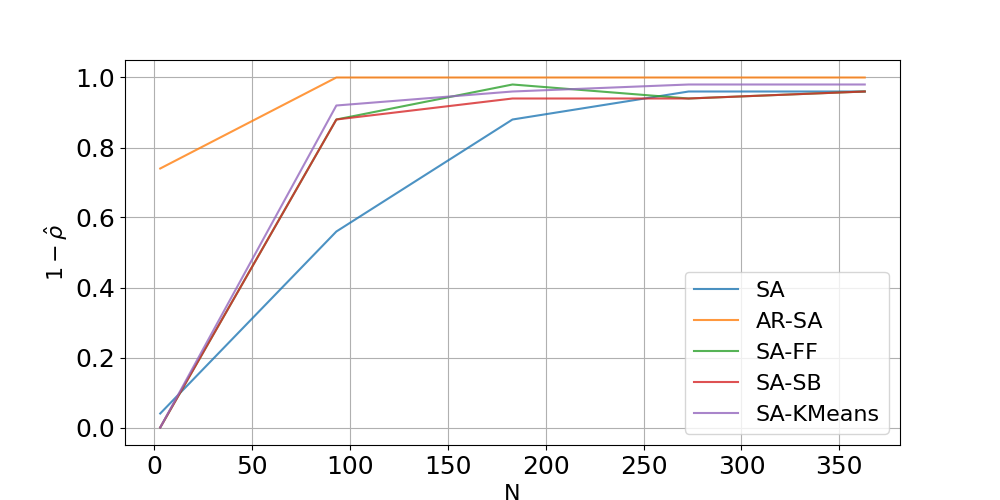
\includegraphics[width=0.95\linewidth]{Dissertation/images/dynamic/washington14/1_beta_N_363_eta_0.01.png}
%   \caption{Empirical reliability %$(1-\hat{\rho})$ 
%   vs. $\#$ samples in CC-OPF for Washington 14 bus, $\eta = 0.01$.}
%   \label{fig:washington14conservatism}
% \end{subfigure}
% \begin{subfigure}{.50\textwidth}
%   \centering
%   % include second image
%   \hspace{-0mm}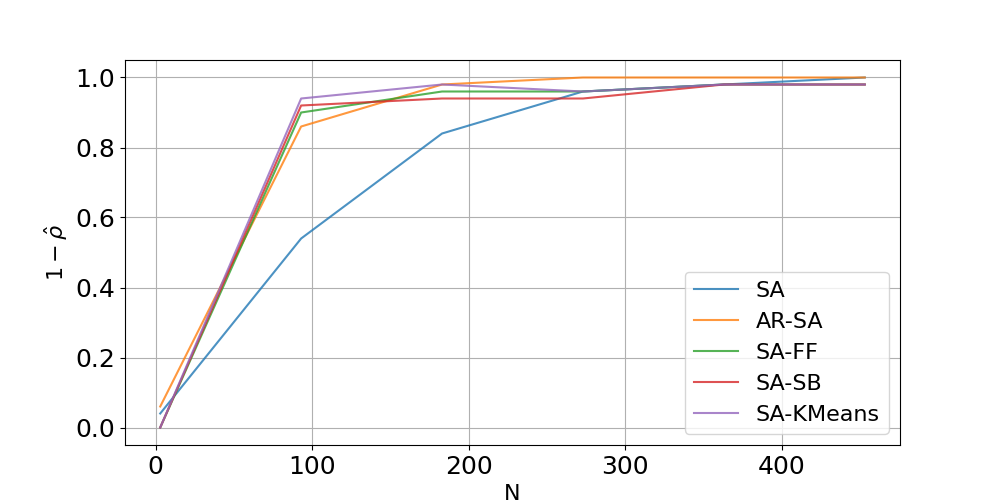
\includegraphics[width=0.95\linewidth]{Dissertation/images/dynamic/ieee30/1_beta_N_453_eta_0.01.png}
%   \caption{Empirical reliability %($1-\hat{\rho}$) 
%   vs $\#$ samples  in CC-OPF for IEEE 30 bus system, $\eta = 0.01$.}
%   \label{fig:ieee30conservatism}
% \end{subfigure}\\
% \begin{subfigure}{.50\textwidth}
%   \centering
%   % include second image
%   \hspace{0mm}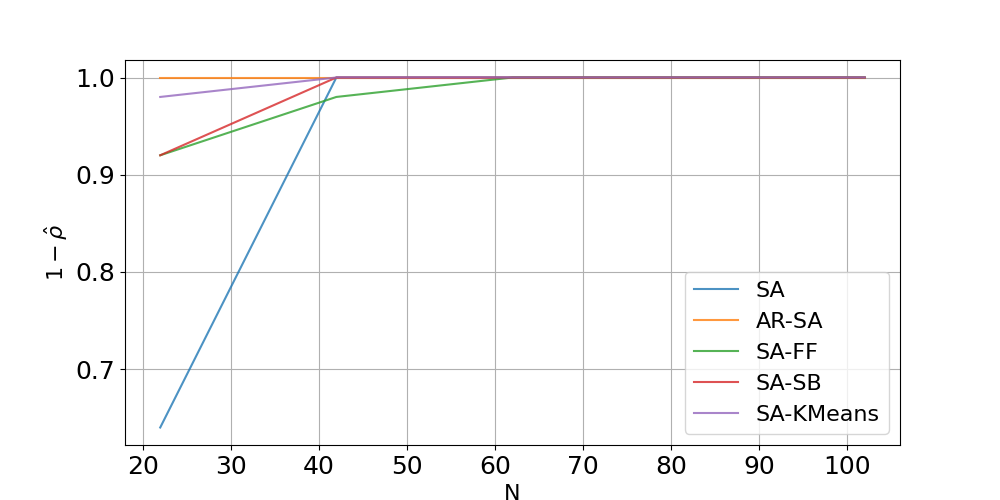
\includegraphics[width=0.95\linewidth]{Dissertation/images/dynamic/grid6/1_beta_N_102_eta_0.1.png}
%   \caption{Empirical reliability %($1-\hat{\rho}$) 
%   vs $\#$ samples  in CC-OPF for Grid6-WW 6 bus system, $\eta = 0.1$.}
%   \label{fig:grid6reliability}
% \end{subfigure}
% \begin{subfigure}{.50\textwidth}
%   \centering
%   % include second image
%   \hspace{0mm}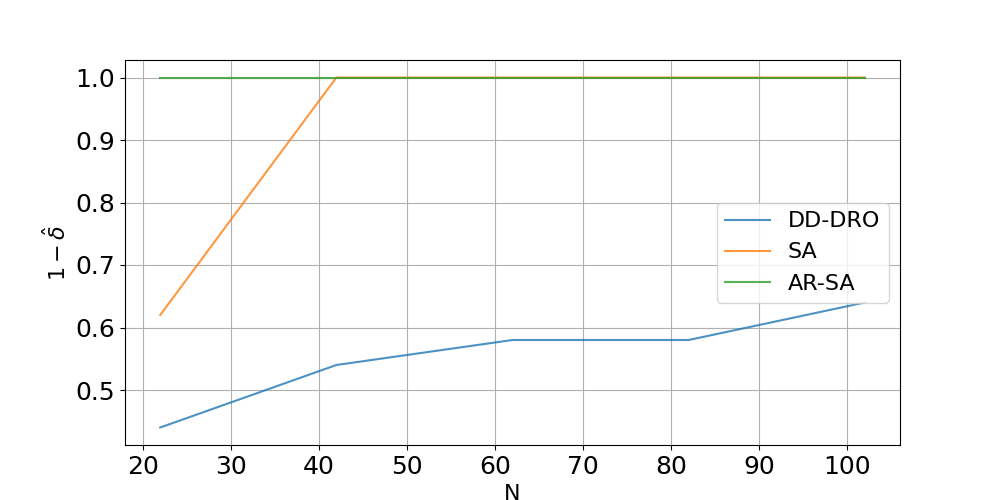
\includegraphics[width=0.95\linewidth]{Dissertation/images/dynamic/grid6/dd-dro/1_beta_N_102_eta_0.1.png}
%   \hspace{0mm}\caption{Empirical reliability  
%   vs $\#$ samples  in CC-OPF for Grid6-WW 6 bus system, $\eta = 0.1$.}
%   \label{fig:grid6reliability-dd-dro}
% \end{subfigure}

% \begin{subfigure}{.50\textwidth}
%   \centering
%   % include first image
% \hspace{10mm}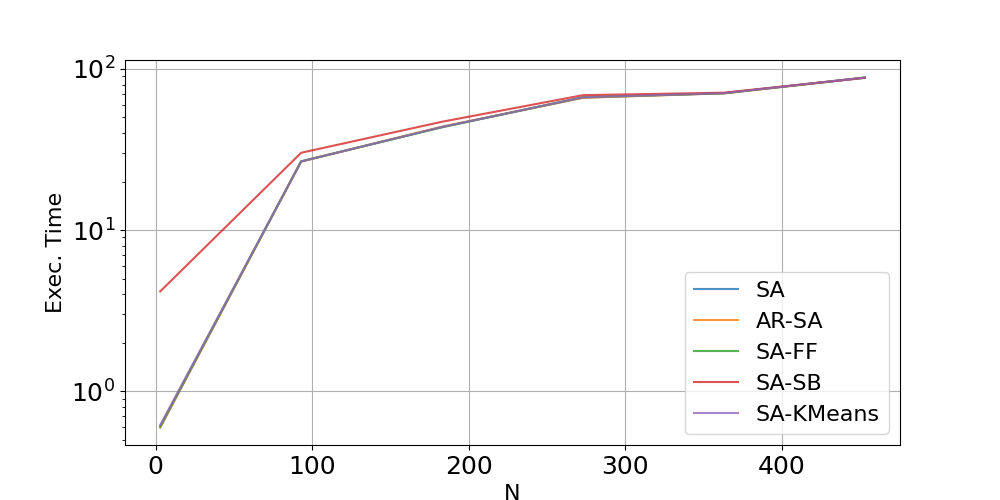
\includegraphics[width=0.95\linewidth]{Dissertation/images/dynamic/ieee30/exec_time_N_453_eta_0.01.png}~~~~~~\hfill
%   \caption{Exec. time vs $\#$ samples, IEEE 30 bus, $\eta = 0.01$.
%   }
%   \label{fig:ieee30time}
% \end{subfigure}
% \begin{subfigure}{.50\textwidth}
%   \centering
%   % include first image
% \hspace{10mm}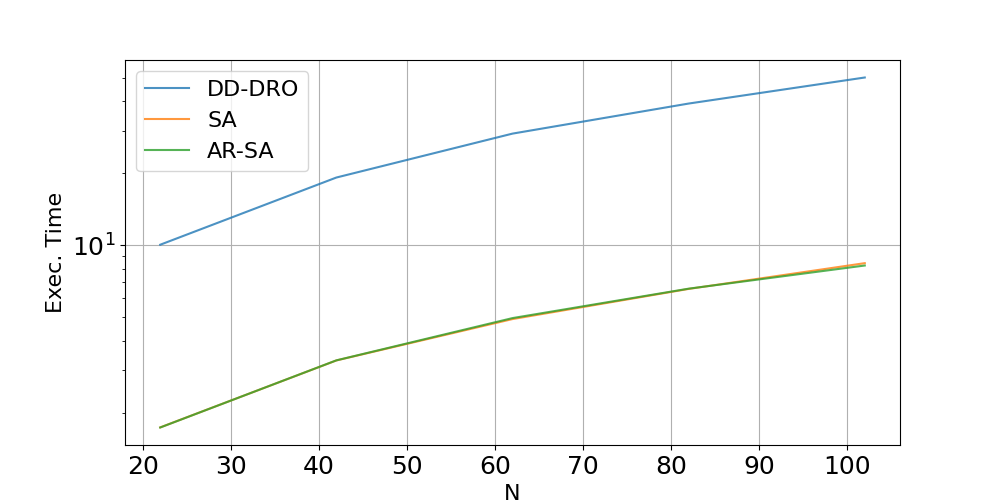
\includegraphics[width=0.95\linewidth]{Dissertation/images/dynamic/grid6/dd-dro/exec_time_N_102_eta_0.1.png}~~~~~~\hfill
%   \caption{Exec. time vs $\#$ samples, Grid6-WW bus, $\eta = 0.1$.
%   }
%   \label{fig:grid6time-dd-dro}
% \end{subfigure}

% \vspace{-7mm}

% \caption{(a, b, d) Empirical reliability ($1-\hat{\rho}$). (e, c, f) Execution time for IEEE-30 and Grid6-WW. The empirical estimates are computed with $L = 200$ optimization instances (for $1-\hat{\rho}$), and $N_{MC}=10^4$ Monte-Carlo samples for each instance to determine constraint validation (for box-plot of $(\hat{\mathbb{P}}_N)_l$).  
% }
% \label{fig:dyn_ieee118}
% \end{figure}

% \newpage

Finally, the chapter concludes in Secion 5.7. Data-driven approximations are beneficial for chance-constrained stochastic programs with unknown uncertainty distributions or JCC settings. However, data demands can quickly become unmanageable with increasing size and reliability requirements. To address this, we proposed a novel method to identify and eliminate redundant scenarios in stochastic approximations for JCC dynamic multi-timestamp DC-OPF. We validate this approach theoretically and demonstrate its high empirical performance across various test cases.

% The \textbf{conclusions chapter} summarizes the thesis consolidates the presented results and offers a concise summary of the investigation’s significance
\section*{Conclusion}
\begin{enumerate}
    \item The adaptive importance sampling algorithm combined with the mirror descent optimization method for usage in power systems has been proposed. The use case is the estimation of the current generation regime's reliability against Gaussian perturbations.
        The algorithm's convergence and validity have been proven theoretically by stating and demonstrating a convergence theorem for optimizing the estimate's variance. The theoretical result underscores algorithm efficiency with $O\left( \sqrt{\log J} \right)$ scaling for the number of constraints $J$.
        The effectiveness and potential advantages of this novel approach have been demonstrated by providing an extensive comparison of its performance with practical algorithms, such as pmvnorm and ALOE, in power systems. Further development in this direction exists as well. The algorithm can be generalized to non-linear settings by using a sampling technique in the complement of convex sets (Grid Walk, Rejection Sampling) and using convex restrictions, see, e.g., \cite{lee2019convex}.
        
    \item A new, significantly more efficient method for constructing scenario approximations has been proposed in the case of Gaussian additive uncertainty with application to power systems optimization - OPF, which is a fundamental routine for operating a power grid. The theoretical guarantees for this new method have been proven. They ensure its mathematical soundness and reliability, indicating a sound reduction in data samples, i.e., scenario usage in scenario approximations in comparison to proven classical results. The performance of the new scenario approximation method in power systems has been demonstrated by comparing it with classical Monte Carlo-based approaches to highlight its data efficiency and accuracy in providing solutions for Joint Chance-Constrained (JCC) problems which are known to have no analytical formulation in general, requiring on average 2 times less data samples (scenarios) than classical approaches. Further prospects in this direction include generalization to non-linear settings, keeping uncertainties' additivity.
    \item An a priori approach to reduce the size of scenario approximations for non-Gaussian multiplicative uncertainty in the setting of dynamic optimal power flow with automatic generation control (AGC) has been proposed. The proposed approach has greatly enhanced computational efficiency and accuracy of the resulting reduced scenario approximation. 
    %Also, the normality of generation-demand mismatch using real time series data from various sources of load and renewable generation
    The effectiveness and reliability of this a priori approach have been confirmed by proving formal statements on its validity in reducing scenario approximations.
    The superior performance and practical applicability of this a priori approach have been demonstrated by comparing it with other scenario reduction methods, including data-driven distributional robust optimization. The experiments have shown that the proposed approach allows to reduce up to a half of scenarios without corrupting the scenario approximation and does not introduce additional exhaustive computations. The further developments can be applications and generalization to a non-linear setting for multiplicative uncertainty.
\end{enumerate}
\section*{Publications on the dissertation contents}

\begin{enumerate}
    \item \fullcite{lukashevich2021importance}
    \item \fullcite{lukashevich2021power}
    \item \fullcite{lukashevich2023importance}
\end{enumerate}

\section*{Other publications by the author}
\begin{enumerate}
    \item \fullcite{shevchenko2023climate}
    \item \fullcite{morozov2023cmip}
    \item \fullcite{mitrovic2023gp}
    \item \fullcite{mitrovic2023fast}
    \item \fullcite{mitrovic2023data}
    \item \fullcite{dvurechensky2022hyperfast}
    \item \fullcite{agafonov2021accelerated}
    \item \fullcite{tanuishkina2024scirep}
\end{enumerate}

\printbibliography[heading=subbibliography]

\ifnumequal{\value{contnumfig}}{1}{\counterwithout{figure}{chapter}}{\counterwithin{figure}{chapter}}
\ifnumequal{\value{contnumtab}}{1}{\counterwithout{table}{chapter}}{\counterwithin{table}{chapter}}


% \pdfbookmark{Общая характеристика работы}{characteristic}             % Закладка pdf
\section*{Общая характеристика работы}

\newcommand{\actuality}{\pdfbookmark[1]{Актуальность}{actuality}\underline{\textbf{\actualityTXT}}}
\newcommand{\progress}{\pdfbookmark[1]{Разработанность темы}{progress}\underline{\textbf{\progressTXT}}}
\newcommand{\aim}{\pdfbookmark[1]{Цели}{aim}\underline{{\textbf\aimTXT}}}
\newcommand{\tasks}{\pdfbookmark[1]{Задачи}{tasks}\underline{\textbf{\tasksTXT}}}
\newcommand{\aimtasks}{\pdfbookmark[1]{Цели и задачи}{aimtasks}\aimtasksTXT}
\newcommand{\novelty}{\pdfbookmark[1]{Научная новизна}{novelty}\underline{\textbf{\noveltyTXT}}}
\newcommand{\influence}{\pdfbookmark[1]{Практическая значимость}{influence}\underline{\textbf{\influenceTXT}}}
\newcommand{\methods}{\pdfbookmark[1]{Методология и методы исследования}{methods}\underline{\textbf{\methodsTXT}}}
\newcommand{\defpositions}{\pdfbookmark[1]{Положения, выносимые на защиту}{defpositions}\underline{\textbf{\defpositionsTXT}}}
\newcommand{\reliability}{\pdfbookmark[1]{Достоверность}{reliability}\underline{\textbf{\reliabilityTXT}}}
\newcommand{\probation}{\pdfbookmark[1]{Апробация}{probation}\underline{\textbf{\probationTXT}}}
\newcommand{\contribution}{\pdfbookmark[1]{Личный вклад}{contribution}\underline{\textbf{\contributionTXT}}}
\newcommand{\publications}{\pdfbookmark[1]{Публикации}{publications}\underline{\textbf{\publicationsTXT}}}

\input{common/characteristic} % Характеристика работы по структуре во введении и в автореферате не отличается (ГОСТ Р 7.0.11, пункты 5.3.1 и 9.2.1), потому её загружаем из одного и того же внешнего файла, предварительно задав форму выделения некоторым параметрам

%Диссертационная работа была выполнена при поддержке грантов \dots

%\underline{\textbf{Объем и структура работы.}} Диссертация состоит из~введения,
%четырех глав, заключения и~приложения. Полный объем диссертации
%\textbf{ХХХ}~страниц текста с~\textbf{ХХ}~рисунками и~5~таблицами. Список
%литературы содержит \textbf{ХХX}~наименование.

\pdfbookmark{Содержание работы}{description}                          % Закладка pdf
\section*{Содержание работы}
Во \underline{\textbf{введении}} обосновывается актуальность
исследований, проводимых в~рамках данной диссертационной работы,
приводится обзор научной литературы по~изучаемой проблеме,
формулируется цель, ставятся задачи работы, излагается научная новизна
и практическая значимость представляемой работы. В~последующих главах
сначала описывается общий принцип, позволяющий \dots, а~потом идёт
апробация на частных примерах: \dots  и~\dots.


\underline{\textbf{Первая глава}} посвящена \dots

картинку можно добавить так:
\begin{figure}[ht]
    \centerfloat{
        \hfill
        \subcaptionbox{\LaTeX}{%
            
\includegraphics[scale=0.27]{latex}}
        \hfill
        \subcaptionbox{Knuth}{%
            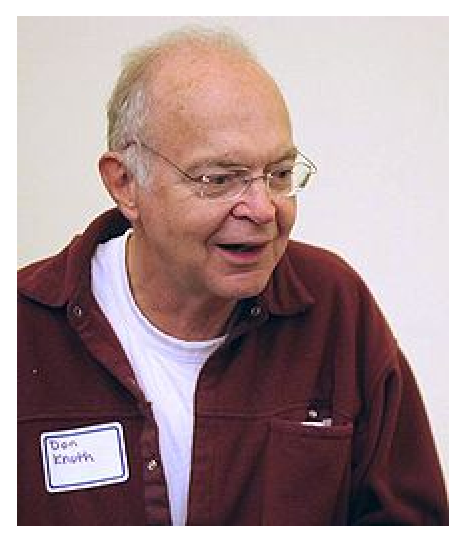
\includegraphics[width=0.25\linewidth]{knuth1}}
        \hfill
    }
    \caption{Подпись к картинке.}\label{fig:latex}
\end{figure}

Формулы в строку без номера добавляются так:
\[
    \lambda_{T_s} = K_x\frac{d{x}}{d{T_s}}, \qquad
    \lambda_{q_s} = K_x\frac{d{x}}{d{q_s}},
\]

\underline{\textbf{Вторая глава}} посвящена исследованию

\underline{\textbf{Третья глава}} посвящена исследованию

Можно сослаться на свои работы в автореферате. Для этого в файле
\verb!Synopsis/setup.tex! необходимо присвоить положительное значение
счётчику \verb!\setcounter{usefootcite}{1}!. В таком случае ссылки на
работы других авторов будут подстрочными.
Изложенные в третьей главе результаты опубликованы в~\cite{vakbib1, vakbib2}.
Использование подстрочных ссылок внутри таблиц может вызывать проблемы.

В \underline{\textbf{четвертой главе}} приведено описание

\FloatBarrier
\pdfbookmark{Заключение}{conclusion}                                  % Закладка pdf
В \underline{\textbf{заключении}} приведены основные результаты работы, которые заключаются в следующем:
%% Согласно ГОСТ Р 7.0.11-2011:
%% 5.3.3 В заключении диссертации излагают итоги выполненного исследования, рекомендации, перспективы дальнейшей разработки темы.
%% 9.2.3 В заключении автореферата диссертации излагают итоги данного исследования, рекомендации и перспективы дальнейшей разработки темы.
\begin{enumerate}
  \item На основе анализа \ldots
  \item Численные исследования показали, что \ldots
  \item Математическое моделирование показало \ldots
  \item Для выполнения поставленных задач был создан \ldots
\end{enumerate}


\pdfbookmark{Литература}{bibliography}                                % Закладка pdf
При использовании пакета \verb!biblatex! список публикаций автора по теме
диссертации формируется в разделе <<\publications>>\ файла
\verb!common/characteristic.tex!  при помощи команды \verb!\nocite!

\ifdefmacro{\microtypesetup}{\microtypesetup{protrusion=false}}{} % не рекомендуется применять пакет микротипографики к автоматически генерируемому списку литературы
\urlstyle{rm}                               % ссылки URL обычным шрифтом
\ifnumequal{\value{bibliosel}}{0}{% Встроенная реализация с загрузкой файла через движок bibtex8
    \renewcommand{\bibname}{\large \bibtitleauthor}
    \nocite{*}
    \insertbiblioauthor           % Подключаем Bib-базы
    %\insertbiblioexternal   % !!! bibtex не умеет работать с несколькими библиографиями !!!
}{% Реализация пакетом biblatex через движок biber
    % Цитирования.
    %  * Порядок перечисления определяет порядок в библиографии (только внутри подраздела, если `\insertbiblioauthorgrouped`).
    %  * Если не соблюдать порядок "как для \printbibliography", нумерация в `\insertbiblioauthor` будет кривой.
    %  * Если цитировать каждый источник отдельной командой --- найти некоторые ошибки будет проще.
    %
    %% authorvak
    \nocite{vakbib1}%
    \nocite{vakbib2}%
    %
    %% authorwos
    \nocite{wosbib1}%
    %
    %% authorscopus
    \nocite{scbib1}%
    %
    %% authorpathent
    \nocite{patbib1}%
    %
    %% authorprogram
    \nocite{progbib1}%
    %
    %% authorconf
    \nocite{confbib1}%
    \nocite{confbib2}%
    %
    %% authorother
    \nocite{bib1}%
    \nocite{bib2}%

    \ifnumgreater{\value{usefootcite}}{0}{
        \begin{refcontext}[labelprefix={}]
            \ifnum \value{bibgrouped}>0
                \insertbiblioauthorgrouped    % Вывод всех работ автора, сгруппированных по источникам
            \else
                \insertbiblioauthor      % Вывод всех работ автора
            \fi
        \end{refcontext}
    }{
        \ifnum \totvalue{citeexternal}>0
            \begin{refcontext}[labelprefix=A]
                \ifnum \value{bibgrouped}>0
                    \insertbiblioauthorgrouped    % Вывод всех работ автора, сгруппированных по источникам
                \else
                    \insertbiblioauthor      % Вывод всех работ автора
                \fi
            \end{refcontext}
        \else
            \ifnum \value{bibgrouped}>0
                \insertbiblioauthorgrouped    % Вывод всех работ автора, сгруппированных по источникам
            \else
                \insertbiblioauthor      % Вывод всех работ автора
            \fi
        \fi
        %  \insertbiblioauthorimportant  % Вывод наиболее значимых работ автора (определяется в файле characteristic во второй section)
        \begin{refcontext}[labelprefix={}]
            \insertbiblioexternal            % Вывод списка литературы, на которую ссылались в тексте автореферата
        \end{refcontext}
        % Невидимый библиографический список для подсчёта количества внешних публикаций
        % Используется, чтобы убрать приставку "А" у работ автора, если в автореферате нет
        % цитирований внешних источников.
        \printbibliography[heading=nobibheading, section=0, env=countexternal, keyword=biblioexternal, resetnumbers=true]%
    }
}
\ifdefmacro{\microtypesetup}{\microtypesetup{protrusion=true}}{}
\urlstyle{tt}                               % возвращаем установки шрифта ссылок URL
      % Содержание автореферата

%%% Выходные сведения типографии
\newpage\thispagestyle{empty}

\vspace*{0pt plus1fill}

\small
\begin{center}
    \textit{\thesisAuthor}
    \par\medskip

    \thesisTitle
    \par\medskip

    Автореф. дис. на соискание ученой степени \thesisDegreeShort
    \par\bigskip

    Подписано в печать \blank[\widthof{999}].\blank[\widthof{999}].\blank[\widthof{99999}].
    Заказ № \blank[\widthof{999999999999}]

    Формат 60\(\times\)90/16. Усл. печ. л. 1. Тираж 50 экз.
    %Это не совсем формат А5, но наиболее близкий, подробнее: http://ru.wikipedia.org/w/index.php?oldid=78976454

    Типография \blank[0.5\linewidth]
\end{center}
\cleardoublepage

\end{document}
